% This template is translated by .... <3
%%%%%%%%%%%%%%%%%%%%%%%%%%%%%%%%%%%%%%%%%%%%%%%%%%%%%%%
\documentclass[13pt,oneside]{article} % 
\usepackage{fontspec} % XeLaTeX
\setmainfont{TeX Gyre Termes}
\usepackage[fontsize=13pt]{scrextend} % Set fontsize=13pt
%\usepackage[paperheight=29.7cm,paperwidth=21cm,right=2cm,left=3cm,top=2cm,bottom=2.5cm]{geometry}% Chuẩn A4, căn lề phải, trái, trên, dưới.
\usepackage[a4paper,right=2cm,left=3cm,top=2cm,bottom=2cm]{geometry}% Chuẩn A4, căn lề phải, trái, trên, dưới.
\usepackage{graphicx} 
\usepackage{float} 
\usepackage{tikz}
\usetikzlibrary{calc,positioning,arrows.meta,fit,shapes.geometric}
\usepackage{indentfirst} 
\renewcommand{\baselinestretch}{1.2} % Line space 1.2
\setlength{\parskip}{6pt} % Spacing after
\setlength{\parindent}{1cm} % Set khoảng cách thụt đầu dòng mỗi đoạn
\usepackage{titlesec} 
\setcounter{secnumdepth}{4} % 4 Heading
\titlespacing*{\section}{0pt}{0pt}{30pt} % Heading 1
\titleformat*{\section}{\fontsize{16pt}{19.2pt}\selectfont \bfseries \centering}

\titlespacing*{\subsection}{0pt}{10pt}{0pt} % Heading 2
\titleformat*{\subsection}{\fontsize{14pt}{16.8pt}\selectfont \bfseries}

\titlespacing*{\subsubsection}{0pt}{10pt}{0pt} % Heading 3
\titleformat*{\subsubsection}{\fontsize{13pt}{15.6pt}\selectfont \bfseries \itshape}

\titlespacing*{\paragraph}{0pt}{10pt}{0pt} % Heading 4
\titleformat*{\paragraph}{\fontsize{13pt}{15.6pt}\selectfont \itshape}

\renewcommand{\figurename}{\fontsize{12pt}{0pt}\selectfont \itshape Hình}
\renewcommand{\thefigure}{\thesection.\arabic{figure}}
\usepackage[font=it]{caption}
\captionsetup[figure]{labelsep=space, justification=centering, singlelinecheck=true, skip=4pt}

\renewcommand{\tablename}{\fontsize{12pt}{0pt}\selectfont \itshape Bảng}
\renewcommand{\thetable}{\thesection.\arabic{table}}
\captionsetup[table]{labelsep=space, justification=centering, singlelinecheck=true, skip=4pt}

\usepackage{multicol,multirow,tabularx}
\usepackage{longtable}
\setlength{\LTpre}{6pt}
\setlength{\LTpost}{6pt}
\newenvironment{fitlongtable}[1]
  {\begingroup\small\setlength{\tabcolsep}{3pt}\begin{longtable}{#1}}
  {\end{longtable}\endgroup}
\usepackage{enumitem}
\setlist{topsep=0pt, partopsep=0pt, parsep=0pt, itemsep=2pt}
\newcolumntype{s}{>{\hsize=.3\hsize}X}
\newcolumntype{y}{>{\hsize=.4\hsize}X}
\newcolumntype{d}{>{\hsize=.1\hsize}X}
\newcolumntype{a}{>{\hsize=1.1\hsize}X}
\newcolumntype{g}{>{\hsize=5\hsize}X}
\newcolumntype{C}[1]{>{\hsize=#1\hsize\centering\arraybackslash}X}
\newcolumntype{R}[1]{>{\hsize=#1\hsize\raggedleft\arraybackslash}X}
\newcolumntype{L}[1]{>{\hsize=#1\hsize\raggedright\arraybackslash}X}
\renewcommand{\tabularxcolumn}[1]{>{\small}m{#1}}

\renewcommand{\theequation}{\thesection.\arabic{equation}}
\newtheorem{theorem}{Theorem}[section]
\newtheorem{defn}[theorem]{Defenition}
\newtheorem{corollary}[theorem]{Corollary}
\newtheorem{lemma}[theorem]{Lemma}

\usepackage{lipsum} % Thư viện tạo chữ linh tinh.
\renewcommand{\contentsname}{MỤC LỤC}
\renewcommand{\listfigurename}{DANH MỤC HÌNH}
\renewcommand{\listtablename}{DANH MỤC BẢNG}
\renewcommand{\refname}{TÀI LIỆU THAM KHẢO}

\usepackage[unicode]{hyperref}
\usepackage{colortbl}
\definecolor{LightCyan}{rgb}{0.88,1,1}
\usepackage{forloop}
\newcounter{loopcntr}
\newcommand{\rpt}[2][1]{\forloop{loopcntr}{0}{\value{loopcntr}<#1}{#2}}

\usepackage[ddmmyyyy]{datetime}
\usepackage{amsmath}
\usepackage{amssymb}
\usepackage{nameref}
\usepackage{rotating}
\usepackage{bm}
\DeclareRobustCommand{\vect}[1]{\bm{#1}}
\pdfstringdefDisableCommands{%
  \renewcommand{\vect}[1]{#1}%
}

\begin{document}

\newgeometry{a4paper,right=2cm,left=3cm,top=2cm,bottom=2cm}

\thispagestyle{empty}

\begin{tikzpicture}[overlay,remember picture]
\draw [line width=3pt]
    ($ (current page.north west) + (3.0cm,-2.0cm) $)
    rectangle
    ($ (current page.south east) + (-2.0cm,2.2cm) $);
\draw [line width=0.5pt]
    ($ (current page.north west) + (3.1cm,-2.1cm) $)
    rectangle
    ($ (current page.south east) + (-2.1cm,2.3cm) $); 
\end{tikzpicture}
\begin{center}
\vspace{-12pt} HỌC VIỆN KỸ THUẬT MẬT MÃ \\
\textbf{\fontsize{14pt}{0pt}\selectfont KHOA CÔNG NGHỆ THÔNG TIN}
\vspace{0.7cm}
 \begin{figure}[H]
     \centering
     
\includegraphics[width=0.28\textwidth]{Figures/logo-KMA.png}
 \end{figure}
\vspace{0.7cm}
\textbf{\fontsize{25pt}{0pt}\selectfont ĐỒ ÁN TỐT NGHIỆP}
\vspace{1cm}
\end{center}
\begin{center}
    \textbf{\fontsize{23pt}{0pt}\selectfont Xây dựng hệ thống bỏ phiếu điện tử sử dụng công nghệ chuỗi khối }
\vspace{7pt}
\begin{table}[H]
    \centering
    \begin{tabular}{c c}
    \fontsize{14pt}{0pt}\selectfont {\textbf{Nguyễn Ngọc Tuyền}}    & \fontsize{14pt}{0pt}\selectfont {\textbf{CT060145}}\\
   % {tuyenboy1234@gmail.com} & {} \\
    \newline\\
    \multicolumn{2}{c}{\textbf{Ngành: Công nghệ thông tin}}\\
    \multicolumn{2}{c}{\textbf{Chuyên ngành: Phát triển phần mềm di động}}\\
    
\end{tabular}
\end{table}
\vspace{1.5cm}
\begin{table}[H]
    \centering
    \begin{tabular}{l l}
{\fontsize{12pt}{14pt}\selectfont\itshape Người hướng dẫn:} & {\fontsize{12pt}{14pt}\selectfont\itshape TS. Phạm Văn Hưởng -- Học viện Kỹ thuật mật mã}\\
{} & {\fontsize{12pt}{14pt}\selectfont\itshape ThS. Ngô Việt Phương -- Công ty Công nghệ thông tin VNPT} \\
\end{tabular}
\end{table}
\vspace{1.5cm}
 \fontsize{14pt}{0pt}\selectfont Hà Nội, 06-2026
\end{center}
\clearpage



%\thispagestyle{empty}
\thispagestyle{empty}

\begin{center}
\vspace{-12pt} HỌC VIỆN KỸ THUẬT MẬT MÃ \\
\textbf{\fontsize{14pt}{0pt}\selectfont KHOA CÔNG NGHỆ THÔNG TIN}
\vspace{0.7cm}
 \begin{figure}[H]
     \centering
     
\includegraphics[width=0.28\textwidth]{Figures/logo-KMA.png}
 \end{figure}
\vspace{0.7cm}
\textbf{\fontsize{25pt}{0pt}\selectfont ĐỒ ÁN TỐT NGHIỆP}
\vspace{1cm}
\end{center}
\begin{center}
    \textbf{\fontsize{23pt}{0pt}\selectfont Xây dựng hệ thống bỏ phiếu điện tử sử dụng công nghệ chuỗi khối }
\vspace{7pt}
\begin{table}[H]
    \centering
    \begin{tabular}{c c}
    \fontsize{14pt}{0pt}\selectfont {\textbf{Nguyễn Ngọc Tuyền}}    & \fontsize{14pt}{0pt}\selectfont {\textbf{CT060229}}\\
   % {tuyenboy1234@gmail.com} & {} \\
    \newline\\
    \multicolumn{2}{c}{\textbf{Ngành: Công nghệ thông tin}}\\
    \multicolumn{2}{c}{\textbf{Chuyên ngành: Phát triển phần mềm di động}}\\
    
\end{tabular}
\end{table}
\vspace{1.5cm}
\begin{table}[H]
    \centering
    \begin{tabular}{l l}
{\fontsize{12pt}{14pt}\selectfont\itshape Người hướng dẫn:} & {\fontsize{12pt}{14pt}\selectfont\itshape TS. Phạm Văn Hưởng -- Học viện Kỹ thuật mật mã}\\
{} & {\fontsize{12pt}{14pt}\selectfont\itshape ThS. Ngô Việt Phương -- Công ty Công nghệ thông tin VNPT} \\
\end{tabular}
\end{table}
\vspace{1.5cm}
 \fontsize{14pt}{0pt}\selectfont Hà Nội, 06-2026
\end{center}
\clearpage
\restoregeometry
 
 
\pagenumbering{roman}
\setcounter{page}{2}
%\input{G-T topic} 
\section*{LỜI CAM ĐOAN}
\phantomsection\addcontentsline{toc}{section}{\numberline {}LỜI CAM ĐOAN}

Em xin cam đoan đồ án tốt nghiệp này là kết quả của quá trình tìm hiểu, nghiên cứu và thực hiện của bản thân em dưới sự hướng dẫn của giáo viên hướng dẫn. Các nội dung, số liệu và kết quả trình bày trong đồ án được em tổng hợp, xây dựng và kiểm chứng một cách trung thực, phù hợp với phạm vi đề tài.

Đồ án tốt nghiệp với đề tài \textbf{Xây dựng hệ thống bỏ phiếu điện tử sử dụng công nghệ chuỗi khối} được thực hiện dựa trên sự tìm hiểu, nghiên cứu của bản thân em cùng với sự hỗ trợ từ giáo viên hướng dẫn. Các tài liệu, số liệu tham khảo được trích dẫn đầy đủ và rõ ràng theo quy định.

Em xin hoàn toàn chịu trách nhiệm về nội dung của đồ án này.

\vspace{6pt}
\hspace{7cm}Hà Nội, ngày \hspace{0.3cm} tháng 06 năm 2026

\hspace{9cm}\textbf{SINH VIÊN}

\vspace{2cm}
\hspace{7.5cm}\textbf{NGUYỄN NGỌC TUYỀN}

%\cleardoublepage
\clearpage
 

\section*{LỜI CẢM ƠN}
\phantomsection\addcontentsline{toc}{section}{\numberline {}LỜI CẢM ƠN}

Trong suốt quá trình thực hiện đồ án tốt nghiệp, em đã nhận được sự hướng dẫn tận tình và hỗ trợ quý báu từ các thầy cô. Em xin gửi lời cảm ơn chân thành và sâu sắc nhất đến thầy \textbf{TS. Phạm Văn Hưởng} và cô \textbf{ThS. Ngô Việt Phương} -- những người đã trực tiếp hướng dẫn, định hướng nghiên cứu và góp ý kịp thời cho em trong suốt thời gian thực hiện đề tài. Sự tận tâm và những chỉ dẫn quý giá của thầy cô là nền tảng quan trọng giúp em hoàn thành đồ án này.

Em cũng xin bày tỏ lòng biết ơn đến toàn thể quý thầy cô trong Khoa đã truyền đạt cho em những kiến thức nền tảng vững chắc trong suốt quá trình học tập. Những kiến thức về kiến trúc và triển khai nền tảng blockchain \textbf{Hyperledger Fabric}, các thuật toán bảo mật hiện đại, cơ chế \textbf{chữ ký số tập thể mù dựa trên lược đồ EC-Schnorr}, cùng các kỹ năng lập trình và thiết kế hệ thống mà em được trang bị trong quá trình học đã trực tiếp phục vụ cho việc nghiên cứu và xây dựng hệ thống trong đề tài này.

Mặc dù đã cố gắng hết sức, đồ án chắc chắn còn nhiều thiếu sót về cả nội dung lẫn hình thức trình bày. Em rất mong nhận được sự góp ý, chỉ dẫn từ quý thầy cô và các bạn để đề tài được hoàn thiện hơn. Những nhận xét đó sẽ là bài học quý giá giúp em tiếp tục rèn luyện và phát triển trong thời gian tới.

Em xin chân thành cảm ơn!

\clearpage



\tableofcontents 


\cleardoublepage

\section*{DANH MỤC TỪ VIẾT TẮT}
\phantomsection \addcontentsline{toc}{section}{\numberline {} DANH MỤC TỪ VIẾT TẮT}

\begin{fitlongtable}{ p{0.13\textwidth} p{0.40\textwidth} p{0.40\textwidth} }
    \textbf{Viết tắt} & \textbf{Thuật ngữ tiếng Anh} & \textbf{Diễn giải} \\
    \hline
    \endhead
    AES & Advanced Encryption Standard & Chuẩn mã hóa tiên tiến \\
    API & Application Programming Interface & Giao diện lập trình ứng dụng \\
    BFF & Backend for Frontend & Tầng máy chủ trung gian cho ứng dụng phía người dùng \\
    BFT & Byzantine Fault Tolerance & Khả năng chịu lỗi Byzantine \\
    CA & Certificate Authority & Tổ chức cấp chứng chỉ số \\
    CLI & Command Line Interface & Giao diện dòng lệnh \\
    CORS & Cross-Origin Resource Sharing & Cơ chế chia sẻ tài nguyên giữa các miền \\
    CSS & Cascading Style Sheets & Ngôn ngữ định kiểu trình bày \\
    DI & Dependency Injection & Tiêm phụ thuộc \\
    DLT & Distributed Ledger Technology & Công nghệ sổ cái phân tán \\
    DOM & Document Object Model & Mô hình đối tượng tài liệu \\
    DTO & Data Transfer Object & Đối tượng truyền dữ liệu \\
    EC & Elliptic Curve & Đường cong elliptic \\
    ECC & Elliptic Curve Cryptography & Mật mã đường cong elliptic \\
    ECDLP & Elliptic Curve Discrete Logarithm Problem & Bài toán logarit rời rạc trên đường cong elliptic \\
    GCM & Galois/Counter Mode & Chế độ mã hóa Galois/Counter \\
    HTTP & Hypertext Transfer Protocol & Giao thức truyền tải siêu văn bản \\
    HTTPS & Hypertext Transfer Protocol Secure & Giao thức truyền tải siêu văn bản an toàn \\
    IaC & Infrastructure as Code & Hạ tầng dạng mã nguồn \\
    IoC & Inversion of Control & Đảo ngược quyền kiểm soát \\
    JSON & JavaScript Object Notation & Định dạng biểu diễn đối tượng JavaScript \\
    JWT & JSON Web Token & Mã thông báo dạng JSON \\
    LRU & Least Recently Used & Cơ chế thay thế phần tử dùng gần nhất ít nhất \\
    MSP & Membership Service Provider & Trình cung cấp dịch vụ thành viên \\
    mTLS & Mutual Transport Layer Security & Lớp bảo mật truyền tải xác thực hai chiều \\
    MUI & Material UI & Thư viện giao diện Material UI \\
    NIST & National Institute of Standards and Technology & Viện Tiêu chuẩn và Công nghệ Quốc gia Hoa Kỳ \\
    QBFT & Quorum-based Byzantine Fault Tolerance & Đồng thuận chịu lỗi Byzantine dựa trên quorum \\
    RBAC & Role-Based Access Control & Kiểm soát truy cập dựa trên vai trò \\
    REST & Representational State Transfer & Kiến trúc truyền trạng thái biểu diễn \\
    RFC & Request for Comments & Tài liệu đặc tả tiêu chuẩn Internet \\
    RNR & React Native Reusables & Bộ thành phần ``mộc'' React Native \\
    RSA & Rivest-Shamir-Adleman & Hệ mật mã khóa công khai RSA \\
    SCAI & Smart Contract AI & Phát triển hợp đồng thông minh có trợ giúp AI \\
    SDK & Software Development Kit & Bộ công cụ phát triển phần mềm \\
    SHA & Secure Hash Algorithm & Thuật toán băm an toàn \\
    TCP & Transmission Control Protocol & Giao thức điều khiển truyền vận \\
    TLS & Transport Layer Security & Lớp bảo mật truyền tải \\
    TPS & Transactions Per Second & Số giao dịch xử lý mỗi giây \\
    TTL & Time To Live & Thời gian sống của bản ghi \\
    UI & User Interface & Giao diện người dùng \\
    UUID & Universally Unique Identifier & Định danh duy nhất toàn cục \\
    XSS & Cross-Site Scripting & Tấn công chèn mã liên miền \\
\end{fitlongtable}

\newpage
 

\input{List-of-figures}

% Tạo danh mục bảng biểu.
{\let\oldnumberline\numberline
\renewcommand{\numberline}{Bảng~\oldnumberline}
\listoftables}
\phantomsection\addcontentsline{toc}{section}{\numberline {} DANH MỤC BẢNG}
\newpage



\pagenumbering{arabic} % Đánh số thứ tự 1,2,3...
\section*{LỜI MỞ ĐẦU}
\phantomsection\addcontentsline{toc}{section}{\numberline {}LỜI MỞ ĐẦU}
Trong bối cảnh chuyển đổi số đang diễn ra mạnh mẽ, công nghệ thông tin đã trở thành nền tảng quan trọng trong hầu hết các lĩnh vực của đời sống xã hội. Một trong những ứng dụng tiêu biểu là bầu cử điện tử, nơi các quy trình đăng ký, bỏ phiếu và kiểm phiếu được thực hiện qua môi trường số, nâng cao tính thuận tiện và khả năng tiếp cận của cử tri. Tuy nhiên, bầu cử có yêu cầu rất cao về tính minh bạch, công bằng, toàn vẹn dữ liệu và bảo mật thông tin cá nhân. Việc ứng dụng blockchain vào bầu cử điện tử mở ra hướng tiếp cận phù hợp nhờ đặc tính phân tán, khó sửa đổi, có thể kiểm chứng công khai và giảm sự phụ thuộc vào một trung tâm quản lý duy nhất.

Các hệ thống bầu cử điện tử truyền thống tồn tại nhiều hạn chế. Dữ liệu phiếu bầu được lưu trữ tập trung nên có nguy cơ bị tấn công hoặc chỉnh sửa nếu máy chủ quản lý bị xâm nhập. Quy trình kiểm phiếu phụ thuộc vào đơn vị vận hành, khiến cử tri khó tự mình xác minh tính đúng đắn của kết quả. Ngoài ra, hệ thống cũ còn gặp thách thức trong việc đảm bảo đồng thời hai yêu cầu tưởng như mâu thuẫn: xác thực đúng tư cách cử tri và giữ bí mật tuyệt đối lựa chọn của họ, dẫn đến các rủi ro như bỏ phiếu trùng lặp, giả mạo danh tính hoặc lộ thông tin cá nhân nhạy cảm.

Từ những vấn đề trên, em đề xuất đề tài \textbf{Xây dựng hệ thống bỏ phiếu điện tử sử dụng công nghệ chuỗi khối}. Đề tài hướng đến xây dựng mô hình bầu cử điện tử có tính an toàn, minh bạch và khả năng kiểm chứng cao, dựa trên hai công nghệ cốt lõi: \textbf{Hyperledger Fabric Blockchain} và \textbf{chữ ký số tập thể mù dựa trên lược đồ EC-Schnorr}. Blockchain cho phép ghi nhận phiếu bầu dưới dạng các giao dịch bất biến, đảm bảo toàn vẹn dữ liệu và hạn chế nguy cơ chỉnh sửa trái phép. Đồng thời, cơ chế chữ ký số tập thể mù xác thực quyền bỏ phiếu mà không làm lộ nội dung lá phiếu, bảo vệ tính riêng tư và ẩn danh của cử tri. Sự kết hợp này góp phần nâng cao khả năng chống gian lận, tăng cường tính minh bạch và củng cố niềm tin vào kết quả bầu cử.

Mục tiêu của đề tài là xây dựng hệ thống hỗ trợ các chức năng cốt lõi gồm đăng ký cử tri, xác thực tư cách tham gia, bỏ phiếu trực tuyến, ghi nhận phiếu bầu lên blockchain, kiểm phiếu tự động và xác minh phiếu bầu sau bầu cử. Đề tài hướng đến một giải pháp vừa đáp ứng yêu cầu kỹ thuật về bảo mật, vừa phù hợp với nhu cầu thực tiễn trong tổ chức bầu cử hiện đại.
\newpage
\clearpage
 
\section*{CHƯƠNG 1. TỔNG QUAN VỀ CÁC CÔNG NGHỆ NỀN TẢNG}
\addcontentsline{toc}{section}{\numberline{}CHƯƠNG 1. TỔNG QUAN VỀ CÁC CÔNG NGHỆ NỀN TẢNG}
\setcounter{section}{1}
\setcounter{subsection}{0}
\setcounter{figure}{0}
\setcounter{table}{0}

\subsection{Tổng quan về Blockchain}

\subsubsection{Khái niệm Blockchain}

Blockchain (chuỗi khối) là một công nghệ lưu trữ và truyền tải thông tin dưới dạng các khối (block) được liên kết với nhau theo trình tự thời gian thông qua các giá trị băm (hash) mật mã, tạo thành một chuỗi dữ liệu liên tục và khó có thể bị chỉnh sửa. Về bản chất, blockchain là một dạng sổ cái phân tán (distributed ledger) được nhân bản và đồng bộ trên nhiều nút (node) trong mạng ngang hàng (peer-to-peer), trong đó mọi thay đổi của dữ liệu đều phải được xác thực thông qua một cơ chế đồng thuận chung trước khi được ghi nhận chính thức vào hệ thống.

Khái niệm blockchain lần đầu tiên được giới thiệu vào năm 2008 trong bài báo \textit{``Bitcoin: A Peer-to-Peer Electronic Cash System''} của tác giả ẩn danh Satoshi Nakamoto, với mục tiêu xây dựng một hệ thống tiền điện tử có khả năng vận hành mà không cần đến bên trung gian tin cậy như ngân hàng hay tổ chức tài chính. Đến tháng 01 năm 2009, mạng Bitcoin chính thức đi vào hoạt động, đánh dấu sự ra đời của ứng dụng blockchain đầu tiên trong thực tế. Từ đó, blockchain dần phát triển vượt ra khỏi phạm vi tiền điện tử và được nghiên cứu, ứng dụng trong nhiều lĩnh vực khác như tài chính, y tế, quản lý chuỗi cung ứng, định danh số, và đặc biệt là các hệ thống bỏ phiếu điện tử.

Cơ chế hoạt động cốt lõi của blockchain dựa trên ba thành phần chính: (1) một sổ cái được phân tán trên nhiều nút mạng, (2) các kỹ thuật mật mã đảm bảo tính toàn vẹn và xác thực dữ liệu, và (3) một giao thức đồng thuận giúp các bên không hoàn toàn tin cậy lẫn nhau có thể thống nhất về trạng thái chung của hệ thống. Khi một giao dịch mới phát sinh, giao dịch đó được lan truyền tới các nút trong mạng, được kiểm tra tính hợp lệ, sau đó được gom thành khối và gắn vào chuỗi hiện có thông qua quá trình đồng thuận. Khi một khối đã được thêm vào, việc sửa đổi nội dung của nó là vô cùng khó khăn vì sẽ làm thay đổi toàn bộ chuỗi giá trị băm phía sau, đòi hỏi phải tính toán lại và đạt được đồng thuận từ phần lớn các nút trong mạng.

Nhờ những đặc điểm phi tập trung, gần như không thể bị sửa đổi và có khả năng kiểm chứng công khai, blockchain được xem là một trong những công nghệ nền tảng quan trọng của cuộc cách mạng công nghiệp lần thứ tư. Công nghệ này mở ra hướng tiếp cận mới cho việc thiết kế các hệ thống đòi hỏi mức độ tin cậy cao mà không cần đến cơ chế quản lý tập trung truyền thống.

\subsubsection{Đặc điểm cơ bản của Blockchain}

Blockchain sở hữu một số đặc điểm nền tảng giúp nó trở nên khác biệt rõ rệt so với các mô hình cơ sở dữ liệu tập trung truyền thống. Những đặc điểm này không chỉ là ưu thế về mặt kỹ thuật mà còn là cơ sở để xây dựng các ứng dụng yêu cầu mức độ tin cậy và an toàn cao như bỏ phiếu điện tử.

\begin{itemize}
    \item \textbf{Tính phân tán (Decentralization):} Khác với mô hình tập trung – nơi toàn bộ dữ liệu được lưu trữ và quản lý bởi một máy chủ duy nhất, dữ liệu trong blockchain được nhân bản và lưu trữ trên nhiều nút độc lập trong mạng ngang hàng. Mỗi nút đều giữ một bản sao đầy đủ hoặc một phần của sổ cái, do đó hệ thống không có điểm yếu trung tâm và vẫn có thể hoạt động bình thường ngay cả khi một số nút bị tấn công hoặc ngừng hoạt động.

    \item \textbf{Tính bất biến (Immutability):} Sau khi một khối được thêm vào chuỗi và được xác nhận bởi mạng lưới, nội dung của khối đó gần như không thể bị thay đổi. Mỗi khối chứa giá trị băm của khối trước đó, tạo thành một liên kết mật mã chặt chẽ. Mọi thay đổi nhỏ trong dữ liệu của một khối sẽ làm thay đổi giá trị băm của nó, kéo theo việc tất cả các khối tiếp sau cũng phải được tính toán lại. Để thực hiện được điều này, kẻ tấn công phải kiểm soát được phần lớn năng lực tính toán hoặc phần lớn các nút xác thực trong mạng, điều gần như không khả thi đối với các blockchain có quy mô lớn.

    \item \textbf{Tính minh bạch (Transparency):} Trong các blockchain công khai, mọi giao dịch đều được ghi lại và có thể được kiểm tra bởi bất kỳ người dùng nào. Mỗi cá nhân tham gia mạng có quyền tra cứu lịch sử giao dịch, từ đó có khả năng tự xác minh tính đúng đắn của dữ liệu mà không cần phải tin tưởng vào một bên thứ ba. Đây là đặc điểm rất phù hợp với các hệ thống đòi hỏi khả năng kiểm tra độc lập, chẳng hạn như bầu cử điện tử.

    \item \textbf{Tính bảo mật và toàn vẹn (Security and Integrity):} Blockchain sử dụng nhiều kỹ thuật mật mã hiện đại như hàm băm, mã hóa khóa công khai và chữ ký số để bảo vệ dữ liệu. Mỗi giao dịch được ký số bằng khóa bí mật của người gửi và chỉ có thể được xác minh thông qua khóa công khai tương ứng, đảm bảo nguồn gốc và tính toàn vẹn của thông tin được lan truyền trong mạng.

    \item \textbf{Tính có thể kiểm chứng (Verifiability):} Mọi giao dịch trên blockchain đều có thể được kiểm chứng độc lập bởi bất kỳ thành viên nào trong mạng. Nhờ cấu trúc chuỗi khối liên kết bằng hàm băm, người dùng có thể xác minh xem một giao dịch nào đó có thực sự nằm trong khối được tuyên bố hay không mà không cần phải tin cậy vào bên trung gian.

    \item \textbf{Tính đồng thuận (Consensus):} Các nút trong mạng blockchain phải đạt được sự thống nhất về trạng thái chung của sổ cái thông qua một giao thức đồng thuận xác định. Điều này đảm bảo rằng dữ liệu được ghi nhận là nhất quán giữa các nút và không xảy ra hiện tượng chia tách hay xung đột dữ liệu.
\end{itemize}

\subsubsection{Cấu trúc dữ liệu Blockchain}

Dữ liệu trong blockchain được tổ chức dưới dạng một chuỗi tuần tự các khối được liên kết bằng giá trị băm. Cấu trúc này được thiết kế nhằm đảm bảo các thuộc tính toàn vẹn, bất biến và có khả năng kiểm chứng. Các thành phần cốt lõi của cấu trúc dữ liệu blockchain bao gồm khối (block), giao dịch (transaction), hàm băm (hash) và cây Merkle (Merkle Tree).

\begin{itemize}
    \item \textbf{Block (Khối):} Mỗi khối là một đơn vị dữ liệu cơ bản của blockchain, thường gồm hai phần là phần đầu (header) và phần thân (body). Phần đầu chứa các trường thông tin quan trọng như: số phiên bản, dấu thời gian (timestamp), giá trị băm của khối trước đó (previous hash), giá trị gốc của cây Merkle (Merkle root), độ khó (difficulty) và giá trị ngẫu nhiên nonce (nếu áp dụng cơ chế Proof of Work). Phần thân chứa danh sách các giao dịch đã được xác nhận trong khối. Việc liên kết giữa khối hiện tại và khối trước thông qua giá trị băm tạo ra một chuỗi liên tục, trong đó khối đầu tiên được gọi là khối khởi tạo (genesis block).

    \item \textbf{Transaction (Giao dịch):} Giao dịch là đơn vị thông tin được ghi nhận trên blockchain, thể hiện một hành động giữa các bên tham gia như chuyển tiền, lưu trữ dữ liệu hoặc thực thi hợp đồng thông minh. Mỗi giao dịch thường bao gồm thông tin về người gửi, người nhận, nội dung, dấu thời gian và chữ ký số. Chữ ký số được dùng để xác thực nguồn gốc và đảm bảo rằng giao dịch không bị giả mạo trong quá trình truyền tải trên mạng.

    \item \textbf{Hash (Hàm băm):} Hàm băm mật mã là thành phần cốt lõi tạo nên tính an toàn của blockchain. Hàm băm nhận một đầu vào có độ dài tùy ý và sinh ra một chuỗi đầu ra có độ dài cố định, mang tính một chiều, không thể đảo ngược và có tính chống va chạm cao. Trong blockchain, các giao dịch và khối được biểu diễn bằng giá trị băm để đảm bảo tính toàn vẹn. Các thuật toán băm phổ biến được sử dụng bao gồm SHA-256 (trong Bitcoin) và Keccak-256 (trong Ethereum). Mọi thay đổi nhỏ trong dữ liệu đầu vào – dù chỉ một bit – đều dẫn đến sự thay đổi đáng kể trong giá trị đầu ra, giúp dễ dàng phát hiện các nỗ lực can thiệp.

    \item \textbf{Merkle Tree (Cây Merkle):} Cây Merkle là một cấu trúc dữ liệu dạng cây nhị phân, trong đó mỗi nút lá lưu trữ giá trị băm của một giao dịch, và mỗi nút cha lưu giá trị băm được tính từ hai nút con. Giá trị băm tại gốc cây – gọi là Merkle root – là một bản tóm lược của toàn bộ giao dịch trong khối. Nhờ cấu trúc này, việc kiểm chứng xem một giao dịch có thuộc khối hay không có thể được thực hiện hiệu quả thông qua đường dẫn Merkle (Merkle proof), với độ phức tạp chỉ là $O(\log n)$ thay vì $O(n)$. Đây là một trong những yếu tố giúp blockchain có khả năng mở rộng tốt và cho phép các nút nhẹ (light node) xác thực giao dịch mà không cần tải toàn bộ khối.
\end{itemize}

\subsubsection{Phân loại Blockchain}

Dựa trên mức độ phân quyền và phạm vi tham gia của các thực thể trong mạng, blockchain được chia thành ba loại chính: blockchain công khai (Public), blockchain riêng tư (Private) và blockchain liên hợp (Consortium).

\begin{itemize}
    \item \textbf{Public Blockchain (Blockchain công khai):} Đây là loại blockchain hoàn toàn mở, cho phép bất kỳ ai trên Internet đều có thể tham gia với vai trò người dùng hoặc nút xác thực mà không cần xin phép. Mọi người đều có quyền đọc dữ liệu, gửi giao dịch và tham gia vào quá trình đồng thuận. Public blockchain có mức độ phi tập trung cao nhất và minh bạch nhất, song hiệu năng thường bị hạn chế do phải xử lý số lượng nút lớn và áp dụng các cơ chế đồng thuận tốn nhiều tài nguyên. Các ví dụ tiêu biểu của loại này bao gồm Bitcoin, Ethereum và Litecoin.

    \item \textbf{Private Blockchain (Blockchain riêng tư):} Trái ngược với loại công khai, blockchain riêng tư chỉ cho phép các thành viên đã được xác thực và cấp phép trước mới có thể tham gia. Quyền đọc, ghi và xác thực giao dịch thường do một tổ chức duy nhất kiểm soát, tương tự như mô hình cơ sở dữ liệu nội bộ nhưng được tăng cường bằng cơ chế blockchain. Loại này có ưu điểm về hiệu năng cao, độ trễ thấp và bảo mật thông tin nội bộ, nhưng đánh đổi bằng mức độ phi tập trung thấp hơn. Private blockchain thường được dùng trong nội bộ doanh nghiệp để quản lý các loại dữ liệu nhạy cảm.

    \item \textbf{Consortium Blockchain (Blockchain liên hợp):} Đây là dạng kết hợp giữa hai loại trên, trong đó quyền tham gia mạng được giới hạn trong một nhóm các tổ chức hoặc thực thể đã được phép. Quá trình đồng thuận và xác thực giao dịch được thực hiện bởi một số nút được chỉ định, thay vì toàn bộ thành viên mạng. Mô hình này cân bằng giữa tính bảo mật, hiệu năng và mức độ tin cậy, phù hợp với các ứng dụng đòi hỏi nhiều bên tham gia mà không hoàn toàn tin cậy lẫn nhau, ví dụ như các nền tảng tài chính liên ngân hàng, quản lý chuỗi cung ứng, hay các hệ thống bỏ phiếu điện tử. Hyperledger Fabric, Corda và Quorum là các nền tảng tiêu biểu thuộc nhóm consortium blockchain.
\end{itemize}

\subsubsection{Cơ chế đồng thuận}

Cơ chế đồng thuận (consensus mechanism) là thành phần thiết yếu của blockchain, giúp các nút trong mạng đạt được sự thống nhất về thứ tự và nội dung của các giao dịch được ghi nhận vào sổ cái. Đây là yếu tố then chốt giúp hệ thống chống lại các hành vi gian lận và đảm bảo tính nhất quán của dữ liệu trên toàn mạng, ngay cả khi một số nút có thể không trung thực hoặc gặp lỗi.

\begin{itemize}
    \item \textbf{Proof of Work (PoW):} Đây là cơ chế đồng thuận đầu tiên được áp dụng trong Bitcoin. Các nút trong mạng (thợ đào – miner) phải thực hiện một bài toán tính toán phức tạp nhằm tìm ra giá trị nonce sao cho giá trị băm của khối nhỏ hơn một ngưỡng nhất định. Nút nào tìm ra trước sẽ có quyền tạo khối mới và nhận phần thưởng tương ứng. PoW có tính an toàn cao nhưng tiêu tốn nhiều năng lượng và có tốc độ xử lý giao dịch tương đối thấp.

    \item \textbf{Proof of Stake (PoS):} Trong cơ chế này, quyền tạo khối được phân bổ dựa trên lượng tài sản (stake) mà nút sở hữu và đặt cọc trong hệ thống, thay vì dựa vào năng lực tính toán. PoS tiêu tốn ít năng lượng hơn nhiều so với PoW và có khả năng mở rộng tốt hơn. Ethereum đã chính thức chuyển từ PoW sang PoS vào năm 2022 thông qua sự kiện The Merge.

    \item \textbf{Practical Byzantine Fault Tolerance (PBFT):} PBFT là cơ chế đồng thuận phù hợp với các blockchain riêng tư hoặc liên hợp, trong đó các nút trao đổi thông điệp qua nhiều vòng để đạt được sự nhất quán. PBFT có khả năng chịu đựng tới một phần ba số nút bị lỗi hoặc gian lận và đạt được độ trễ thấp. Tuy nhiên, mức độ trao đổi thông điệp tăng nhanh theo số lượng nút, khiến PBFT khó áp dụng cho mạng có quy mô rất lớn.

    \item \textbf{Raft và Proof of Authority (PoA):} Các cơ chế này thường được sử dụng trong các blockchain doanh nghiệp khi số lượng nút có hạn và đã được xác thực danh tính. Hyperledger Fabric, chẳng hạn, sử dụng Raft như một cơ chế sắp xếp giao dịch (ordering service) nhằm đảm bảo thứ tự thống nhất giữa các nút xác thực. PoA cho phép một số nút có thẩm quyền được phép tạo khối mới, đem lại hiệu năng cao và độ trễ thấp, phù hợp với các môi trường có yêu cầu xử lý nhanh.
\end{itemize}

\subsubsection{Smart Contract}

Hợp đồng thông minh (Smart Contract) là một chương trình tự động được lưu trữ và thực thi trên blockchain, có khả năng tự động hóa các điều khoản đã được thỏa thuận giữa các bên tham gia mà không cần đến trung gian. Khái niệm này được đề xuất lần đầu bởi nhà khoa học máy tính Nick Szabo vào năm 1994, song chỉ trở nên phổ biến và được hiện thực hóa rộng rãi từ khi nền tảng Ethereum ra đời vào năm 2015.

Một hợp đồng thông minh bao gồm các đoạn mã chứa các quy tắc, điều kiện và hành động sẽ được thực thi tự động khi các điều kiện đầu vào được đáp ứng. Vì được lưu trữ trên blockchain, hợp đồng thông minh kế thừa các đặc điểm như tính bất biến, tính minh bạch và khả năng kiểm chứng. Sau khi được triển khai, mã của hợp đồng thông minh không thể bị sửa đổi và mọi lần thực thi đều được ghi nhận công khai trên sổ cái.

Trong các nền tảng blockchain hiện đại, hợp đồng thông minh được sử dụng để xây dựng các ứng dụng phi tập trung (Decentralized Applications – dApp) trong nhiều lĩnh vực như tài chính phi tập trung (DeFi), bảo hiểm tự động, đấu giá, định danh số, quản lý tài sản số và các hệ thống bỏ phiếu điện tử. Đối với hệ thống bỏ phiếu, hợp đồng thông minh có thể được sử dụng để định nghĩa các luật bầu cử, tự động kiểm phiếu và đảm bảo rằng quá trình diễn ra theo đúng quy trình đã được công khai từ trước.

Trong nền tảng Hyperledger Fabric, hợp đồng thông minh được hiện thực dưới dạng \textit{chaincode} – một mô-đun phần mềm được viết bằng các ngôn ngữ phổ thông như Go, Java hoặc Node.js. Chaincode được thực thi trong môi trường biệt lập trên các nút xác thực, đảm bảo tính nhất quán giữa các bên tham gia mạng.

\subsubsection{Ưu điểm và hạn chế của Blockchain}

\textit{Ưu điểm:} Blockchain mang lại nhiều lợi ích nổi bật so với các mô hình cơ sở dữ liệu tập trung truyền thống:
\begin{itemize}
    \item Loại bỏ sự phụ thuộc vào bên trung gian tin cậy, giúp giảm thiểu chi phí giao dịch và rủi ro do sự cố từ một điểm tập trung.

    \item Nhờ cơ chế phân tán và đồng thuận, dữ liệu trên blockchain có tính toàn vẹn cao và khó bị giả mạo.

    \item Tính minh bạch của blockchain cho phép mọi thành viên tham gia tự xác minh kết quả, từ đó nâng cao niềm tin trong cộng đồng.

    \item Blockchain hỗ trợ tự động hóa các quy trình thông qua hợp đồng thông minh, giúp giảm sai sót do con người và tăng tốc độ xử lý.

    \item Khả năng truy vết và kiểm tra lịch sử giao dịch giúp blockchain trở nên đặc biệt phù hợp với các ứng dụng đòi hỏi kiểm toán độc lập như tài chính, chuỗi cung ứng và bầu cử điện tử.
\end{itemize}

\textit{Hạn chế:} Bên cạnh các ưu điểm, blockchain vẫn tồn tại một số hạn chế cần được xem xét:
\begin{itemize}
    \item Hiệu năng và khả năng mở rộng còn hạn chế, đặc biệt với các blockchain công khai có lưu lượng giao dịch lớn.

    \item Việc lưu trữ toàn bộ chuỗi khối trên nhiều nút khiến yêu cầu về dung lượng và băng thông tăng nhanh theo thời gian.

    \item Một số cơ chế đồng thuận như PoW tiêu tốn lượng năng lượng đáng kể, gây ảnh hưởng đến môi trường.

    \item Tính bất biến của blockchain – dù là một ưu điểm cốt lõi – cũng đặt ra thách thức khi cần chỉnh sửa các dữ liệu sai sót hoặc tuân thủ các quy định về quyền được lãng quên trong các quy định bảo vệ dữ liệu cá nhân.

    \item Công nghệ blockchain vẫn còn tương đối mới mẻ, khung pháp lý chưa hoàn thiện, và đòi hỏi mức độ chuyên môn cao trong quá trình triển khai cũng như vận hành.
\end{itemize}

Tóm lại, với những đặc tính nổi bật về phân tán, minh bạch, toàn vẹn và khả năng kiểm chứng, blockchain là nền tảng phù hợp để xây dựng các hệ thống có yêu cầu tin cậy cao như bỏ phiếu điện tử. Tuy nhiên, để khai thác tối đa hiệu quả của công nghệ này, việc lựa chọn nền tảng cụ thể, cơ chế đồng thuận và mô hình triển khai cần được cân nhắc kỹ lưỡng. Trong các phần tiếp theo của chương, đồ án sẽ tiếp tục đi sâu vào nền tảng Hyperledger Fabric – một blockchain liên hợp tiêu biểu được sử dụng trong hệ thống đề xuất.

\subsection{Tổng quan về Hyperledger Fabric}

\subsubsection{Giới thiệu Hyperledger Fabric}

Hyperledger Fabric là một nền tảng công nghệ sổ cái phân tán (Distributed Ledger Technology -- DLT) mã nguồn mở, được thiết kế ở cấp độ doanh nghiệp (enterprise-grade) và được điều phối phát triển bởi dự án Hyperledger thuộc Quỹ Linux (Linux Foundation). Khác với các blockchain công khai như Bitcoin hay Ethereum -- vốn hướng tới một mạng lưới mở, không cần cấp phép và sử dụng tiền điện tử làm động lực kinh tế -- Hyperledger Fabric được xây dựng để phục vụ các kịch bản hợp tác giữa các tổ chức (B2B), nơi các bên tham gia đã được định danh rõ ràng và cần một cơ sở hạ tầng tin cậy để chia sẻ dữ liệu, thực thi quy trình nghiệp vụ và lưu trữ bằng chứng về các giao dịch chung.

Hyperledger Fabric được khởi động vào năm 2015 với sự đóng góp ban đầu từ IBM và một số tập đoàn công nghệ lớn, sau đó liên tục được phát triển qua nhiều phiên bản. Các phiên bản từ \textit{v2.x} trở đi đã hoàn thiện đáng kể về kiến trúc, quản trị hợp đồng thông minh và hiệu năng; phiên bản \textit{v3.x} tiếp tục mở rộng hỗ trợ các cơ chế đồng thuận chịu lỗi Byzantine (BFT). Nhờ tính chất là mạng có cấp phép (permissioned), hỗ trợ kênh giao dịch riêng tư và bảo mật dữ liệu mức cao, Hyperledger Fabric đã được ứng dụng rộng rãi trong các lĩnh vực tài chính -- ngân hàng, chuỗi cung ứng, y tế, chính phủ điện tử và đặc biệt phù hợp với các bài toán cần kiểm soát danh tính và quyền hạn chặt chẽ như hệ thống bỏ phiếu điện tử.

Trong khuôn khổ của đồ án, Hyperledger Fabric được lựa chọn làm nền tảng triển khai do khả năng đáp ứng đồng thời các yêu cầu về tính phi tập trung trong xác thực, định danh người dùng dựa trên chứng chỉ số và khả năng xử lý số lượng phiếu lớn với độ trễ thấp.

\subsubsection{Đặc điểm của Hyperledger Fabric}

So với các nền tảng blockchain phổ biến khác, Hyperledger Fabric có một số đặc điểm cốt lõi giúp nó trở thành nền tảng phù hợp cho các hệ thống doanh nghiệp đòi hỏi mức độ tin cậy và bảo mật cao:

\begin{itemize}
    \item \textbf{Mạng lưới cấp quyền (Permissioned Network):} Mọi thực thể tham gia mạng -- bao gồm người dùng, ứng dụng khách, nút xác thực và nút sắp xếp giao dịch -- đều phải được định danh thông qua chứng chỉ số do Cơ quan cấp chứng chỉ (Certificate Authority -- CA) phát hành. Điều này loại bỏ tính ẩn danh, cho phép thiết lập trách nhiệm pháp lý rõ ràng và phù hợp với các môi trường kinh doanh đòi hỏi tuân thủ pháp luật.

    \item \textbf{Kiến trúc mô-đun (Modular Architecture):} Hyperledger Fabric được thiết kế theo hướng các thành phần có thể \textit{cắm rút} (pluggable), bao gồm cơ chế đồng thuận, hệ thống quản lý danh tính, cơ sở dữ liệu trạng thái và môi trường thực thi hợp đồng thông minh. Tính mô-đun này cho phép các tổ chức tùy biến nền tảng theo nhu cầu nghiệp vụ thay vì phải chấp nhận một mô hình cứng nhắc.

    \item \textbf{Hiệu năng và khả năng mở rộng (High Performance and Scalability):} Quá trình thực thi hợp đồng thông minh được tách biệt khỏi quá trình đồng thuận, giúp các giao dịch được xử lý song song trên nhiều nút và sau đó mới được sắp xếp theo thứ tự. Cách tiếp cận này giúp Hyperledger Fabric đạt được tốc độ xử lý hàng nghìn giao dịch mỗi giây với độ trễ chỉ ở mức vài trăm mili giây, vượt trội so với các blockchain công khai sử dụng cơ chế đào.

    \item \textbf{Tính bảo mật và riêng tư cao (Confidentiality):} Hyperledger Fabric hỗ trợ chia sẻ dữ liệu có chọn lọc thông qua hai cơ chế chính: kênh giao tiếp riêng tư (Channels) và bộ dữ liệu riêng tư (Private Data Collections). Nhờ đó, các đối tác kinh doanh có thể giao dịch trên cùng một mạng nhưng vẫn đảm bảo bí mật dữ liệu của riêng mình đối với các bên không liên quan.

    \item \textbf{Không yêu cầu tiền điện tử (No Native Cryptocurrency):} Khác với Bitcoin hay Ethereum, Hyperledger Fabric không phát hành đồng tiền số nội tại và không sử dụng cơ chế đào (mining). Việc xác thực giao dịch dựa trên chính sách phê duyệt được các tổ chức thống nhất từ trước, qua đó loại bỏ chi phí năng lượng khổng lồ và giúp hệ thống phù hợp với các quy định pháp lý ở nhiều quốc gia.
\end{itemize}

\subsubsection{Kiến trúc tổng thể}

Một trong những điểm khác biệt cơ bản nhất giữa Hyperledger Fabric với các blockchain truyền thống nằm ở mô hình kiến trúc xử lý giao dịch. Trong khi các nền tảng như Bitcoin hay Ethereum sử dụng mô hình \textit{Order -- Execute} -- tức là các giao dịch được sắp xếp trước rồi mới được thực thi tuần tự trên toàn bộ nút mạng -- thì Hyperledger Fabric áp dụng mô hình \textit{Execute -- Order -- Validate} (Thực thi -- Sắp xếp -- Kiểm tra). Theo mô hình này, giao dịch trước tiên được thực thi mô phỏng tại một nhóm nhỏ các nút có thẩm quyền, sau đó kết quả được gửi đến dịch vụ sắp xếp để xếp thứ tự, và cuối cùng các nút trong mạng mới kiểm tra tính hợp lệ trước khi ghi vào sổ cái. Cách tiếp cận này giúp loại bỏ các giao dịch xung đột ngay từ giai đoạn thực thi, đồng thời cho phép xử lý song song nhiều giao dịch không liên quan.

Một đặc điểm quan trọng khác trong kiến trúc của Hyperledger Fabric là \textbf{sự tách biệt vai trò} (Separation of Roles) giữa các loại nút. Thay vì để mỗi nút đảm nhiệm toàn bộ quy trình như trong các blockchain công khai, Hyperledger Fabric tách rời tầng đồng thuận (Ordering Service) khỏi tầng thực thi ứng dụng (Peers). Các nút Peer tập trung vào việc thực thi hợp đồng thông minh, lưu trữ sổ cái và xác thực giao dịch, trong khi các nút Orderer chỉ chịu trách nhiệm sắp xếp giao dịch và tạo khối. Sự chuyên môn hóa này giúp tối ưu hóa băng thông và tài nguyên tính toán, đồng thời cho phép mở rộng độc lập từng tầng tùy theo nhu cầu thực tế.

Về \textbf{cơ chế đồng thuận}, Hyperledger Fabric không cố định một thuật toán duy nhất mà cung cấp khả năng đồng thuận đa tầng có thể cắm rút (Pluggable Consensus). Trong các phiên bản phổ biến hiện nay, dịch vụ sắp xếp thường sử dụng giao thức Raft -- một thuật toán chịu lỗi do sự cố (Crash Fault Tolerant -- CFT) với mô hình lãnh đạo -- người theo. Bên cạnh đó, các phiên bản mới nhất đã bổ sung hỗ trợ các giải pháp chịu lỗi Byzantine (Byzantine Fault Tolerant -- BFT) để đáp ứng các kịch bản đa tổ chức không hoàn toàn tin cậy lẫn nhau, qua đó tăng tính linh hoạt và khả năng áp dụng cho nhiều mô hình quản trị khác nhau.

\subsubsection{Các thành phần chính}

Hyperledger Fabric bao gồm nhiều thành phần được phối hợp chặt chẽ để cấu thành một mạng lưới hoàn chỉnh. Các thành phần cốt lõi bao gồm: nút Peer, dịch vụ sắp xếp Orderer, cơ quan cấp chứng chỉ, kênh giao tiếp và sổ cái.

\begin{itemize}
    \item \textbf{Peer (Nút mạng):} Peer là thành phần cơ bản và trung tâm của mạng Hyperledger Fabric. Mỗi tổ chức tham gia mạng thường vận hành một hoặc nhiều Peer, trực tiếp lưu trữ bản sao của sổ cái và các chaincode đã được triển khai. Dựa trên vai trò trong từng giao dịch, Peer được phân thành hai nhóm chính: \textit{Endorsing Peer} (Nút xác thực) chịu trách nhiệm tiếp nhận đề xuất giao dịch từ Client, thực thi mô phỏng chaincode trên trạng thái sổ cái hiện tại, ký số xác nhận kết quả và gửi phản hồi về cho Client; \textit{Committing Peer} (Nút ghi nhận) nhận các khối giao dịch đã được sắp xếp từ Orderer, kiểm tra lại tính hợp lệ và cập nhật chính thức vào sổ cái cục bộ. Trong thực tế, một Peer có thể đồng thời đảm nhiệm cả hai vai trò trên tùy theo cấu hình của mạng.

    \item \textbf{Orderer (Dịch vụ sắp xếp -- Ordering Service):} Orderer là thành phần đặc thù của Hyperledger Fabric, không tồn tại trong các blockchain công khai theo cách tương tự. Vai trò của Orderer là tiếp nhận các giao dịch đã được xác thực bởi các Endorsing Peer, sắp xếp chúng theo thứ tự thời gian tuyến tính và đóng gói thành các khối (Blocks) với kích thước hoặc khoảng thời gian được cấu hình từ trước. Sau khi tạo khối, Orderer phân phối các khối đến toàn bộ các Committing Peer trong kênh thông qua giao thức truyền tin Gossip, đảm bảo tính nhất quán của sổ cái trên toàn mạng. Do tách biệt khỏi tầng thực thi, dịch vụ sắp xếp có thể được triển khai dưới dạng cụm nhiều nút Orderer để đảm bảo tính sẵn sàng cao và chịu lỗi.

    \item \textbf{Certificate Authority (Cơ quan cấp chứng chỉ -- Fabric CA):} Fabric CA là thành phần đóng vai trò \textit{gốc rễ của lòng tin} (Root of Trust) trong mạng. Cơ quan này cung cấp và quản lý các chứng chỉ số theo chuẩn X.509 cho mọi thực thể trong mạng, bao gồm người dùng cuối, Peer, Orderer và các ứng dụng khách. Bên cạnh chức năng cấp phát chứng chỉ ban đầu, Fabric CA còn hỗ trợ các nghiệp vụ quản lý vòng đời chứng chỉ như gia hạn, thu hồi và quản lý danh sách thu hồi chứng chỉ (CRL). Một mạng Hyperledger Fabric có thể có nhiều CA, mỗi CA thường thuộc về một tổ chức và chịu trách nhiệm cấp danh tính cho các thành viên trong tổ chức đó.

    \item \textbf{Channel (Kênh giao tiếp):} Channel là một cơ chế độc đáo của Hyperledger Fabric, được hình dung như một \textit{đường ống} truyền thông riêng tư kết nối một nhóm các tổ chức cụ thể. Mỗi Channel có sổ cái, tập hợp Peer thành viên, chính sách quản trị và chaincode riêng biệt. Các giao dịch và dữ liệu trao đổi trong một Channel hoàn toàn tách biệt và bí mật đối với các tổ chức không phải là thành viên của Channel đó. Cơ chế này đặc biệt hữu ích trong các kịch bản kinh doanh khi nhiều tổ chức chia sẻ chung một hạ tầng nhưng có những hợp tác song phương hoặc đa phương riêng cần được bảo mật.

    \item \textbf{Ledger (Sổ cái):} Sổ cái của Hyperledger Fabric được cấu thành từ hai phần cốt lõi có tính bổ trợ chặt chẽ. \textit{World State} (Trạng thái hiện tại) lưu trữ giá trị hiện tại của tài sản và dữ liệu nghiệp vụ dưới dạng cặp khóa -- giá trị (key-value), cho phép truy vấn nhanh trạng thái tức thời mà không cần duyệt toàn bộ lịch sử giao dịch. Hyperledger Fabric hỗ trợ hai hệ quản trị cơ sở dữ liệu phổ biến cho World State là LevelDB (mặc định, phù hợp với truy vấn theo khóa đơn giản) và CouchDB (cho phép truy vấn phong phú bằng các biểu thức JSON phức tạp). \textit{Blockchain} (Nhật ký giao dịch) là chuỗi các khối được liên kết bằng giá trị băm theo cơ chế chỉ ghi đè/thêm mới (append-only), lưu trữ toàn bộ lịch sử các giao dịch dẫn đến trạng thái hiện tại. Sự kết hợp này vừa đảm bảo hiệu năng truy vấn cao, vừa giữ được khả năng truy vết và kiểm chứng toàn diện -- một yêu cầu thiết yếu trong các hệ thống đòi hỏi tính minh bạch như bỏ phiếu điện tử.
\end{itemize}

\subsubsection{Chaincode}

Chaincode là cách gọi của Hyperledger Fabric đối với hợp đồng thông minh. Về bản chất, chaincode là một chương trình phần mềm triển khai logic nghiệp vụ đã được các bên tham gia mạng thống nhất, có khả năng đọc và ghi dữ liệu trực tiếp vào World State của sổ cái. Mỗi chaincode thường biểu diễn một loại hợp đồng hoặc một nhóm nghiệp vụ cụ thể như quản lý phiếu bầu, theo dõi tài sản, kiểm tra điều kiện thực hiện giao dịch, v.v.

Khác với Ethereum -- nơi hợp đồng thông minh chạy trong máy ảo Ethereum Virtual Machine (EVM) cùng tiến trình với nút mạng -- chaincode trong Hyperledger Fabric được thực thi trong một môi trường cô lập, thường là một Docker container riêng biệt được khởi tạo bởi Peer khi cần. Sự cô lập này mang lại hai lợi ích quan trọng: bảo vệ Peer khỏi các sự cố hoặc mã độc trong chaincode, và cho phép sử dụng nhiều ngôn ngữ lập trình thông dụng để viết hợp đồng thông minh. Hiện nay, Hyperledger Fabric hỗ trợ chính thức ba ngôn ngữ phổ biến trong doanh nghiệp là Go (Golang), Node.js (JavaScript/TypeScript) và Java. Điều này giúp các nhóm phát triển có thể tận dụng nguồn nhân lực sẵn có thay vì phải đào tạo từ đầu với một ngôn ngữ đặc thù như Solidity.

Từ phiên bản v2.0, Hyperledger Fabric giới thiệu quy trình quản lý vòng đời chaincode mới (Fabric Chaincode Lifecycle), trong đó các bước triển khai chaincode được phân tách rõ ràng và đòi hỏi sự đồng thuận của nhiều tổ chức thay vì chỉ một quản trị viên duy nhất. Quy trình này bao gồm các bước chính: (1) \textit{Đóng gói} (Package) -- chaincode được đóng gói thành một tệp triển khai duy nhất; (2) \textit{Cài đặt} (Install) -- mỗi tổ chức cài đặt gói chaincode lên các Peer của mình; (3) \textit{Phê duyệt} (Approve) -- các tổ chức tham gia kênh đưa ra phê duyệt với định nghĩa chaincode (bao gồm tên, phiên bản, chính sách phê duyệt, v.v.); và (4) \textit{Cam kết} (Commit) -- khi đủ số tổ chức theo chính sách đã phê duyệt, chaincode chính thức được cam kết lên kênh và sẵn sàng phục vụ giao dịch. Cách tổ chức này phản ánh tinh thần quản trị phi tập trung, trong đó mọi thay đổi quan trọng đối với logic nghiệp vụ chung đều phải có sự đồng thuận của các bên liên quan.

\subsubsection{Membership Service Provider}

Membership Service Provider (MSP -- Dịch vụ thành viên) là một thành phần trừu tượng hóa kiến trúc mật mã của Hyperledger Fabric, đóng vai trò cầu nối giữa hệ thống chứng chỉ số do Fabric CA cấp phát và mô hình quản trị phi tập trung của mạng. Trong khi CA chịu trách nhiệm phát hành các chứng chỉ X.509 nhằm chứng minh danh tính của một thực thể, thì MSP định nghĩa cách các chứng chỉ đó được diễn giải thành các \textit{vai trò} và \textit{quyền hạn} cụ thể bên trong một mạng hoặc một kênh.

Cụ thể, MSP cung cấp các thông tin cấu hình như: danh sách CA gốc được tin cậy, danh sách CA trung gian, danh sách thu hồi chứng chỉ (CRL), các quy tắc xác định vai trò (Admin, Client, Peer, Orderer), cũng như các định danh tổ chức được phép tham gia. Khi một thực thể gửi một thông điệp hoặc giao dịch, MSP sẽ kiểm tra chữ ký số đính kèm, đối chiếu với các CA tin cậy và xác định thực thể đó thuộc về tổ chức nào, có vai trò gì và được phép thực hiện những thao tác nào trong ngữ cảnh hiện tại.

Tầm quan trọng của MSP thể hiện ở chỗ nó là cơ sở cho các \textit{Chính sách} (Policies) của Hyperledger Fabric. Mọi quyết định trong mạng -- từ việc ai được phép gọi một chaincode, ai có quyền thay đổi cấu hình kênh, đến chính sách phê duyệt giao dịch -- đều được biểu diễn dưới dạng các tổ hợp logic của các vai trò do MSP định nghĩa. Nhờ đó, Hyperledger Fabric có thể triển khai mô hình quản trị phi tập trung linh hoạt, trong đó quyền lực không tập trung vào một bên duy nhất mà được phân bổ theo các quy tắc đã được công khai thống nhất giữa các tổ chức.

\subsubsection{Quy trình xử lý giao dịch}

Quy trình xử lý giao dịch trong Hyperledger Fabric là sự kết hợp chặt chẽ giữa các thành phần đã trình bày ở trên, thể hiện rõ nét mô hình kiến trúc \textit{Execute -- Order -- Validate}. Một giao dịch điển hình đi qua năm bước chính, từ lúc được khởi tạo bởi ứng dụng phía Client cho đến khi được ghi nhận chính thức vào sổ cái.

\begin{itemize}
    \item \textbf{Bước 1 -- Đề xuất giao dịch (Transaction Proposal):} Ứng dụng phía Client, thông qua bộ thư viện phát triển (SDK) của Hyperledger Fabric, tạo ra một đề xuất giao dịch chứa thông tin về chaincode cần gọi, các tham số đầu vào và danh tính của người gửi. Đề xuất này được ký số bằng chứng chỉ của Client và được gửi tới một tập hợp các Endorsing Peer được xác định theo \textit{Chính sách xác thực} (Endorsement Policy) của chaincode tương ứng.

    \item \textbf{Bước 2 -- Thực thi mô phỏng và ký xác thực (Endorsement):} Mỗi Endorsing Peer nhận được đề xuất sẽ kiểm tra chữ ký, sau đó thực thi mô phỏng chaincode trên trạng thái hiện tại của World State. Kết quả mô phỏng tạo ra một tập dữ liệu đọc/ghi (Read-Write Set -- RW Set), gồm các khóa đã được đọc cùng với phiên bản tương ứng và các khóa dự kiến sẽ được cập nhật cùng giá trị mới. Endorsing Peer ký số lên RW Set và gửi phản hồi (Proposal Response) về cho Client. Một điểm cần lưu ý là ở bước này, không có dữ liệu nào được ghi thực sự vào sổ cái -- toàn bộ chỉ là mô phỏng để xác định tác động tiềm tàng của giao dịch.

    \item \textbf{Bước 3 -- Phát tán giao dịch (Submit Transaction):} Client thu thập đầy đủ các phản hồi từ Endorsing Peer, kiểm tra tính nhất quán giữa các RW Set (các Peer phải đưa ra cùng một kết quả mô phỏng) và đối chiếu với Chính sách xác thực để đảm bảo đã có đủ chữ ký theo yêu cầu. Sau đó, Client đóng gói các phản hồi này thành một thông điệp giao dịch hoàn chỉnh và gửi tới Ordering Service.

    \item \textbf{Bước 4 -- Sắp xếp và đóng khối (Ordering and Batching):} Orderer tiếp nhận các giao dịch từ nhiều Client khác nhau trong cùng một kênh, sắp xếp chúng theo một thứ tự nhất quán dựa trên giao thức đồng thuận đã cấu hình (chẳng hạn Raft), và đóng gói thành các khối mới với kích thước hoặc khoảng thời gian được định trước. Khối sau khi tạo sẽ được phân phối tới toàn bộ Committing Peer trong kênh.

    \item \textbf{Bước 5 -- Xác thực và cập nhật sổ cái (Validation and Commit):} Mỗi Committing Peer khi nhận được khối mới sẽ thực hiện hai bước kiểm tra: kiểm tra chữ ký xác thực có thỏa mãn Endorsement Policy hay không, và kiểm tra tính nhất quán của RW Set với trạng thái hiện tại của World State theo cơ chế kiểm soát đồng thời đa phiên bản (MVCC -- Multi-Version Concurrency Control). Các giao dịch hợp lệ sẽ được cập nhật vào World State, trong khi cả giao dịch hợp lệ và không hợp lệ đều được ghi nhận vào Blockchain dưới dạng bằng chứng lịch sử (kèm theo cờ trạng thái tương ứng). Cuối cùng, Peer phát đi sự kiện (Event) để thông báo kết quả tới ứng dụng phía Client.
\end{itemize}

Mô hình xử lý giao dịch theo kiểu \textit{Execute -- Order -- Validate} này mang lại nhiều ưu thế: cho phép xử lý song song các giao dịch không xung đột, giảm tải cho dịch vụ sắp xếp, và cho phép linh hoạt cấu hình ai có quyền xác thực giao dịch nào thông qua Endorsement Policy. Đặc biệt, trong bối cảnh của hệ thống bỏ phiếu điện tử, mô hình này cho phép thiết kế các chính sách phê duyệt phù hợp -- chẳng hạn yêu cầu chữ ký của nhiều tổ chức giám sát bầu cử cho mỗi phiếu bầu -- mà vẫn đảm bảo hiệu năng tổng thể của hệ thống.

\subsubsection{Ưu điểm và hạn chế của Hyperledger Fabric}

\textit{Ưu điểm:} Là một nền tảng blockchain liên hợp được thiết kế dành riêng cho môi trường doanh nghiệp, Hyperledger Fabric mang lại một số lợi thế nổi bật:

\begin{itemize}
    \item Cung cấp khả năng bảo mật và phân quyền dữ liệu xuất sắc nhờ cơ chế Channel và Private Data Collection, đáp ứng tốt các kịch bản hợp tác giữa nhiều bên với mức độ tin cậy không đồng đều.

    \item Kiến trúc mô-đun hóa cao cho phép doanh nghiệp dễ dàng bảo trì, thay đổi cơ chế đồng thuận hoặc cơ sở dữ liệu trạng thái khi nhu cầu nghiệp vụ thay đổi mà không phải xây dựng lại toàn bộ hệ thống.

    \item Hiệu năng cao với tốc độ xử lý lớn và độ trễ thấp nhờ loại bỏ cơ chế Proof of Work, đồng thời tách biệt quá trình thực thi và sắp xếp giao dịch.

    \item Thân thiện với lập trình viên: các hợp đồng thông minh có thể được viết bằng những ngôn ngữ phổ biến như Go, Java hay Node.js thay vì phải học một ngôn ngữ chuyên biệt, qua đó giảm đáng kể chi phí đào tạo và rút ngắn thời gian phát triển.

    \item Hệ sinh thái phong phú với sự hậu thuẫn của Linux Foundation và nhiều tập đoàn công nghệ lớn, cùng với cộng đồng phát triển năng động và tài liệu kỹ thuật chi tiết.
\end{itemize}

\textit{Hạn chế:} Bên cạnh các ưu điểm, Hyperledger Fabric cũng tồn tại một số hạn chế cần được lưu ý khi triển khai:

\begin{itemize}
    \item Kiến trúc hệ thống tương đối phức tạp với nhiều thành phần phối hợp (Peer, Orderer, CA, MSP, Channel, chaincode, v.v.), tạo ra rào cản học tập (steep learning curve) đáng kể đối với các nhóm phát triển mới làm quen.

    \item Quy trình thiết lập ban đầu và quản trị mạng lưới (Network Governance) giữa nhiều tổ chức đòi hỏi nhiều thời gian và công sức, từ việc thống nhất chính sách, cấp phát chứng chỉ, đến cấu hình kênh và phê duyệt chaincode.

    \item Do là blockchain có cấp phép, Hyperledger Fabric không phù hợp với các bài toán đòi hỏi tính chất công khai hoàn toàn, phi tập trung tuyệt đối và ẩn danh -- chẳng hạn các ứng dụng tiền điện tử mở rộng quy mô toàn cầu.

    \item Việc phụ thuộc vào hạ tầng chứng chỉ số đặt ra yêu cầu cao về bảo mật khóa và quản lý vòng đời chứng chỉ; rò rỉ khóa của một CA có thể gây ảnh hưởng nghiêm trọng tới toàn bộ tổ chức liên quan.
\end{itemize}

Tổng kết lại, Hyperledger Fabric là một nền tảng blockchain doanh nghiệp mạnh mẽ, kết hợp được các yếu tố về bảo mật, hiệu năng, khả năng tùy biến và quản trị phi tập trung. Với cơ chế định danh chặt chẽ, hỗ trợ chữ ký số dựa trên chứng chỉ X.509 và khả năng triển khai chaincode bằng các ngôn ngữ thông dụng, Hyperledger Fabric đặc biệt phù hợp với việc xây dựng hệ thống bỏ phiếu điện tử -- nơi đồng thời cần đảm bảo tính xác thực của cử tri, sự riêng tư của lá phiếu, tính minh bạch trong kiểm phiếu và khả năng kiểm chứng độc lập của các bên giám sát. Đây là lý do nền tảng này được lựa chọn làm hạ tầng triển khai cho hệ thống đề xuất trong đồ án.

\subsection{Cơ sở mật mã học}

Mật mã học hiện đại là nền tảng lý thuyết cho hầu hết các hệ thống bảo mật trên môi trường mạng nói chung và các hệ thống bỏ phiếu điện tử nói riêng. Trong khuôn khổ của đồ án, các nguyên thủy mật mã được sử dụng bao gồm hàm băm mật mã, hệ mật khóa công khai, chữ ký số cùng với mô hình lý thuyết để đánh giá tính an toàn -- mô hình tiên tri ngẫu nhiên (Random Oracle Model -- ROM). Mục này trình bày một cách hệ thống các khái niệm nền tảng nói trên làm cơ sở cho các nội dung được phát triển ở các mục và các chương tiếp theo.

\subsubsection{Hàm băm mật mã}

Hàm băm mật mã (cryptographic hash function) là một hàm toán học $H: \{0,1\}^{*} \rightarrow \{0,1\}^{k}$ nhận đầu vào là một chuỗi bit có độ dài bất kỳ và sinh ra đầu ra có độ dài cố định $k$ (thường là 256 hoặc 512 bit). Giá trị đầu ra $H(M)$ được gọi là \textit{giá trị băm} hay \textit{bản tóm lược} (digest) của thông điệp $M$. Vai trò của hàm băm trong mật mã hiện đại là cung cấp một \textit{vân tay số} (fingerprint) duy nhất, gọn nhẹ và đại diện cho thông điệp gốc, nhờ đó có thể phát hiện mọi thay đổi dù là nhỏ nhất xảy ra với thông điệp ban đầu.

Để được coi là an toàn về mặt mật mã, một hàm băm $H$ phải đồng thời thỏa mãn ba thuộc tính cơ bản sau:

\begin{itemize}
    \item \textbf{Tính kháng tiền ảnh (Preimage Resistance):} Với một giá trị băm $h$ cho trước, không tồn tại thuật toán hiệu quả trong thời gian đa thức tìm được thông điệp $M$ sao cho $H(M) = h$. Thuộc tính này còn được gọi là tính \textit{một chiều} (one-way) của hàm băm.

    \item \textbf{Tính kháng tiền ảnh thứ hai (Second Preimage Resistance):} Cho trước một thông điệp $M_1$, không tồn tại thuật toán hiệu quả tìm được thông điệp $M_2 \neq M_1$ sao cho $H(M_1) = H(M_2)$.

    \item \textbf{Tính kháng xung đột (Collision Resistance):} Không tồn tại thuật toán hiệu quả tìm được hai thông điệp khác nhau $M_1 \neq M_2$ bất kỳ thỏa mãn $H(M_1) = H(M_2)$.
\end{itemize}

Ngoài ra, một hàm băm mật mã tốt còn phải có \textit{tính khuếch tán} (avalanche effect) -- nghĩa là mọi thay đổi nhỏ trong đầu vào, dù chỉ một bit, đều dẫn đến sự thay đổi đáng kể và không thể dự đoán ở đầu ra. Trong thực tế, các thuật toán băm phổ biến hiện nay bao gồm dòng SHA-2 (SHA-256, SHA-512), SHA-3 (Keccak), cùng với các thuật toán đặc thù theo tiêu chuẩn quốc gia như GOST R34.11. Trong các lược đồ chữ ký số, hàm băm được sử dụng để rút gọn thông điệp về kích thước cố định trước khi ký nhằm đảm bảo hiệu năng và tránh các tấn công liên quan đến cấu trúc thông điệp dài.

\subsubsection{Mã hóa khóa công khai}

Hệ mật khóa công khai (Public-Key Cryptosystem) -- hay còn gọi là hệ mật bất đối xứng -- được Whitfield Diffie và Martin Hellman đề xuất lần đầu tiên vào năm 1976 trong bài báo \textit{``New Directions in Cryptography''}, mở ra một hướng đi hoàn toàn mới trong lĩnh vực mật mã hiện đại. Khác với hệ mật đối xứng truyền thống, trong đó cùng một khóa được sử dụng cho cả hai quá trình mã hóa và giải mã, hệ mật khóa công khai sử dụng một \textit{cặp khóa} gồm khóa công khai $pk$ (public key) và khóa bí mật $sk$ (secret key) có quan hệ toán học chặt chẽ nhưng không thể tính khóa bí mật từ khóa công khai trong thời gian hợp lý.

Cơ chế hoạt động cơ bản của hệ mật khóa công khai có thể tóm tắt như sau: khóa công khai được phổ biến rộng rãi và bất kỳ ai cũng có thể sử dụng để mã hóa một thông điệp gửi tới chủ sở hữu của cặp khóa; trong khi đó khóa bí mật được người chủ giữ kín và chỉ người này mới có thể giải mã ngược thông điệp đã được mã hóa bằng khóa công khai tương ứng. Tính an toàn của hệ mật khóa công khai phụ thuộc vào độ khó của một bài toán toán học cụ thể -- gọi là \textit{bài toán cửa sập một chiều} (one-way trapdoor function) -- mà kẻ tấn công nếu không có khóa bí mật thì không thể giải được trong thời gian đa thức.

Năm 1978, R. Rivest, A. Shamir và L. Adleman đã công bố hệ mật RSA -- hệ mật khóa công khai thực tế đầu tiên dựa trên độ khó của bài toán phân tích thừa số nguyên lớn (Integer Factorization Problem -- IFP). Sau đó, hàng loạt hệ mật khóa công khai khác đã được đề xuất dựa trên các bài toán khó khác nhau, tiêu biểu là hệ ElGamal và Schnorr dựa trên bài toán logarit rời rạc (Discrete Logarithm Problem -- DLP), cũng như các hệ mật trên đường cong elliptic (Elliptic Curve Cryptography -- ECC) dựa trên bài toán logarit rời rạc trên đường cong elliptic (Elliptic Curve Discrete Logarithm Problem -- ECDLP). Hệ mật khóa công khai không chỉ giải quyết bài toán bảo mật thông tin mà còn là nền tảng cho các giao thức xác thực, trao đổi khóa và đặc biệt là chữ ký số -- chủ đề trọng tâm của các phần tiếp theo.

\subsubsection{Chữ ký số}

Chữ ký số (Digital Signature -- DS) là một dạng dữ liệu được tạo ra bằng hệ mật khóa công khai nhằm xác thực nguồn gốc và tính toàn vẹn của một thông điệp điện tử. Theo Nghị định số 130/2018/NĐ-CP ngày 27/9/2018 của Chính phủ Việt Nam, chữ ký số được định nghĩa là \textit{``một loại chữ ký điện tử, được tạo bằng sự chuyển đổi thông điệp dữ liệu sử dụng một hệ thống mật mã không đối xứng, theo đó người có được thông điệp dữ liệu ban đầu và khóa công khai của người ký có thể xác định được chính xác việc biến đổi nêu trên được tạo ra bằng đúng khóa bí mật tương ứng với khóa công khai trong cùng một cặp khóa, và sự toàn vẹn nội dung của thông điệp dữ liệu kể từ khi thực hiện việc biến đổi nêu trên''}.

Một lược đồ chữ ký số được xác định bởi bộ ba thuật toán $(Gen, Sig, Ver)$, trong đó:

\begin{itemize}
    \item \textbf{Thuật toán sinh khóa (Gen):} Nhận đầu vào là tham số an toàn $1^k$ và sinh ra cặp khóa công khai -- bí mật $(pk, sk)$. Đây thường là thuật toán xác suất.

    \item \textbf{Thuật toán ký (Sig):} Sử dụng khóa bí mật $sk$ để tạo ra chữ ký $s \leftarrow Sig(sk, M)$ tương ứng với thông điệp $M$. Để tăng hiệu năng và tránh các bất lợi liên quan đến độ dài thông điệp lớn, trong thực tế người ký không ký trực tiếp lên thông điệp $M$ mà ký lên giá trị băm $H(M)$.

    \item \textbf{Thuật toán xác thực (Ver):} Sử dụng khóa công khai $pk$ để kiểm tra tính hợp lệ của cặp $(M, s)$ và trả về kết quả thuộc tập $\{0, 1\}$. Đây là thuật toán khẳng định, cho phép bất kỳ ai có khóa công khai đều có thể kiểm tra chữ ký mà không cần biết khóa bí mật.
\end{itemize}

Quy trình tạo và xác thực chữ ký số được mô tả khái quát như sau: phía người ký áp dụng hàm băm $H$ lên thông điệp $M$ để tạo ra giá trị tóm lược $H(M)$, sau đó sử dụng khóa bí mật của mình để biến đổi $H(M)$ thành chữ ký số $s$. Cặp $(M, s)$ được gửi tới người nhận. Phía người nhận tiến hành tính lại giá trị $H(M)$ từ thông điệp nhận được, đồng thời sử dụng khóa công khai của người gửi để khôi phục hoặc tính giá trị đối chiếu từ chữ ký $s$. Nếu hai giá trị này khớp nhau, chữ ký được kết luận là hợp lệ -- điều này đồng thời chứng tỏ thông điệp xuất phát từ đúng người gửi và không bị thay đổi trong quá trình truyền.

Nhờ cơ chế trên, chữ ký số đảm nhiệm ba chức năng cốt lõi sau: (i) \textit{xác thực nguồn gốc} thông điệp -- chỉ chủ sở hữu khóa bí mật mới có thể tạo ra chữ ký hợp lệ tương ứng với khóa công khai đã được công bố; (ii) \textit{đảm bảo tính toàn vẹn} -- mọi thay đổi dù nhỏ trên thông điệp sẽ làm thay đổi giá trị băm và khiến chữ ký không còn hợp lệ; (iii) \textit{chống chối bỏ} -- người ký không thể phủ nhận hành động ký của mình bởi chỉ có khóa bí mật của họ mới sinh ra được chữ ký đó. Hiện nay, chữ ký số đã được chuẩn hóa và triển khai tại hơn 40 quốc gia trên thế giới thông qua các tiêu chuẩn như FIPS của Hoa Kỳ và GOST của Liên bang Nga. Dựa trên các tiêu chí phân loại khác nhau, các lược đồ chữ ký số đã được phát triển thành nhiều biến thể như chữ ký số nhóm, chữ ký số tập thể, chữ ký số đại diện, chữ ký số ngưỡng và chữ ký số mù -- mỗi biến thể nhằm đáp ứng một yêu cầu nghiệp vụ cụ thể.

\subsubsection{Các yêu cầu an toàn của chữ ký số}

Để được sử dụng trong thực tế, một lược đồ chữ ký số phải chống lại được các dạng tấn công đã biết trên cả hai khía cạnh: khả năng truy cập thông tin của kẻ tấn công và mức độ thành công mà kẻ tấn công có thể đạt được. Goldwasser \textit{et al.} đã hệ thống hóa các loại tấn công và các dạng phá vỡ lược đồ chữ ký số như sau.

\textit{Các loại tấn công} được phân loại theo lượng thông tin mà kẻ tấn công có thể thu thập được:

\begin{itemize}
    \item \textbf{Tấn công vào khóa (Key Only Attacks -- KOA):} Kẻ tấn công chỉ biết khóa công khai của người ký. Đây là dạng tấn công cơ bản nhất.

    \item \textbf{Tấn công văn bản được biết (Known Message Attack -- KMA):} Kẻ tấn công có thể truy cập tới các chữ ký của một số văn bản $M_1, M_2, \dots, M_n$ nhưng không tự ý lựa chọn được các văn bản này.

    \item \textbf{Tấn công văn bản được lựa chọn tổng quát (Generic Chosen Message Attack -- GCMA):} Kẻ tấn công có thể lựa chọn trước một danh sách các văn bản và yêu cầu chữ ký hợp lệ tương ứng. Danh sách này không phụ thuộc vào khóa công khai của người ký.

    \item \textbf{Tấn công văn bản được lựa chọn trực tiếp (Directed Chosen Message Attack -- DCMA):} Tương tự GCMA nhưng danh sách văn bản được tạo ra \textit{sau khi} biết khóa công khai của người ký, tuy nhiên vẫn được tạo trước khi quan sát được bất kỳ chữ ký nào.

    \item \textbf{Tấn công văn bản được lựa chọn thích ứng (Adaptive Chosen Message Attack -- ACMA):} Đây là dạng tấn công nghiêm trọng nhất, trong đó kẻ tấn công có thể sử dụng người ký hợp lệ như một \textit{nguồn Oracle}, lựa chọn văn bản để ký sau khi đã biết khóa công khai và quan sát được các chữ ký trước đó. Một lược đồ chữ ký số khi đưa vào sử dụng phải chứng minh được khả năng chịu được dạng tấn công này.
\end{itemize}

\textit{Các dạng phá vỡ} được phân loại theo mức độ thành công của kẻ tấn công, sắp xếp theo thứ tự giảm dần của mức độ nghiêm trọng:

\begin{itemize}
    \item \textbf{Phá vỡ hoàn toàn (Total Break -- TB):} Kẻ tấn công khôi phục được khóa bí mật của người ký, từ đó có thể giả mạo chữ ký trên bất kỳ thông điệp nào.

    \item \textbf{Giả mạo tổng quát (Universal Forgery -- UF):} Kẻ tấn công xây dựng được một thuật toán có chức năng tương đương với thuật toán ký, dù không nhất thiết phải khôi phục được chính xác khóa bí mật.

    \item \textbf{Giả mạo có lựa chọn (Selective Forgery -- SF):} Kẻ tấn công có thể tạo ra chữ ký hợp lệ cho một thông điệp cụ thể được lựa chọn trước theo ý của họ.

    \item \textbf{Giả mạo có tồn tại (Existential Forgery -- EF):} Kẻ tấn công có thể tạo ra ít nhất một cặp $(M, s)$ hợp lệ, dù thông điệp $M$ có thể không có ý nghĩa thực tế và không được lựa chọn trước.
\end{itemize}

Một lược đồ chữ ký số được coi là \textit{an toàn} (theo nghĩa mạnh nhất hiện nay) nếu nó không bị giả mạo có tồn tại dưới tấn công văn bản lựa chọn thích ứng (existentially unforgeable under adaptive chosen message attack -- EUF-CMA). Đây là tiêu chuẩn an toàn được áp dụng cho hầu hết các lược đồ chữ ký số hiện đại và là mục tiêu cần đạt khi đề xuất các biến thể chữ ký mới như chữ ký mù tập thể được trình bày trong các chương sau của đồ án.

\subsubsection{Mô hình Random Oracle Model}

Việc chứng minh chặt chẽ tính an toàn của một lược đồ chữ ký số là một bài toán phức tạp. Một lược đồ được coi là an toàn nếu khả năng phá vỡ nó \textit{tương đương} (về mặt tính toán) với độ khó của một bài toán toán học đã được chấp nhận là khó -- chẳng hạn như IFP, DLP hay ECDLP. Tuy nhiên, trong nhiều trường hợp, việc thực hiện chứng minh chặt chẽ này trong mô hình tính toán chuẩn (standard model) là rất khó khăn hoặc không khả thi, đặc biệt với các lược đồ sử dụng hàm băm.

Để giải quyết khó khăn nói trên, năm 1993, Mihir Bellare và Phillip Rogaway đã đề xuất \textit{mô hình tiên tri ngẫu nhiên} (Random Oracle Model -- ROM) -- một mô hình lý tưởng hóa cho phép chứng minh tính an toàn một cách nghiêm ngặt cho các giao thức mật mã dựa trên hàm băm. Trong mô hình ROM, hàm băm $H$ không còn được xem là một hàm xác định cụ thể mà được coi là một \textit{tiên tri ngẫu nhiên} (random oracle) -- một hộp đen lý tưởng có hành vi được mô tả như sau: khi nhận một thông điệp $M$ chưa từng được truy vấn, oracle sẽ chọn một giá trị ngẫu nhiên đều trên toàn miền giá trị làm đầu ra; khi $M$ được truy vấn lần thứ hai trở đi, oracle phải \textit{ghi nhớ} và trả về cùng một giá trị đã sinh ra trước đó để đảm bảo tính nhất quán.

Trong khuôn khổ ROM, kẻ tấn công có thể tự do truy vấn oracle để lấy giá trị băm hoặc chữ ký của bất kỳ thông điệp nào mà họ quan tâm (mô phỏng kịch bản tấn công ACMA). Một lược đồ chữ ký số được xem là \textit{không an toàn trong ROM} nếu kẻ tấn công có thể giả mạo được chữ ký cho một thông điệp mà chính họ chưa từng truy vấn tới oracle. Ngược lại, nếu mọi thuật toán hiệu quả trong thời gian đa thức của kẻ tấn công đều có xác suất giả mạo thành công là một hàm vô cùng nhỏ $\varepsilon(k)$ theo tham số an toàn $k$, lược đồ được coi là an toàn trong ROM.

Mặc dù mô hình ROM là một sự lý tưởng hóa -- hàm băm trong thực tế (như SHA-256) không thật sự là một tiên tri ngẫu nhiên -- ROM vẫn là công cụ chứng minh an toàn được sử dụng phổ biến và đáng tin cậy nhất hiện nay đối với các giao thức mật mã thực dụng. Trong các chương tiếp theo, đồ án sẽ sử dụng mô hình ROM làm khung lý thuyết để phân tích và đánh giá tính an toàn của các lược đồ chữ ký mù và chữ ký mù tập thể được đề xuất.

\subsection{Mật mã đường cong elliptic}

Mật mã đường cong elliptic (Elliptic Curve Cryptography -- ECC) được giới thiệu một cách độc lập bởi Neal Koblitz và Victor Miller vào năm 1985, mở ra một hướng đi mới trong việc xây dựng các hệ mật khóa công khai. Khác với các hệ mật cổ điển dựa trên bài toán phân tích thừa số nguyên tố (IFP) hay bài toán logarit rời rạc (DLP) trên trường hữu hạn, mật mã đường cong elliptic dựa trên độ khó của bài toán logarit rời rạc trên nhóm các điểm của đường cong elliptic (ECDLP) -- một bài toán cho đến nay vẫn chưa có giải thuật hiệu quả thời gian đa thức. Ưu điểm nổi bật của ECC là cung cấp mức độ an toàn tương đương các hệ mật truyền thống nhưng với độ dài khóa ngắn hơn nhiều lần, do đó tiết kiệm tài nguyên tính toán, băng thông truyền dẫn và năng lượng tiêu thụ. Chính vì lý do đó, ECC đã trở thành nền tảng toán học của hàng loạt chuẩn chữ ký số quốc tế hiện đại như ECDSA, EC-Schnorr và GOST R34.10-2012, đồng thời là cơ sở cho các lược đồ chữ ký mù tập thể được trình bày trong các chương sau của đồ án.

\subsubsection{Khái niệm đường cong elliptic}

Cho $K$ là một trường hữu hạn có đặc số khác $2$ và $3$. Một \textit{đường cong elliptic} (Elliptic Curve -- EC) trên trường $K$ được định nghĩa là tập hợp tất cả các nghiệm $(x, y) \in K \times K$ của phương trình Weierstrass rút gọn:
\begin{equation}
E: y^2 = x^3 + ax + b
\label{eq:ec-weierstrass}
\end{equation}
cùng với một điểm đặc biệt $\mathcal{O}$ được gọi là \textit{điểm vô cùng} (point at infinity), trong đó các hệ số $a, b \in K$ thỏa mãn điều kiện không suy biến:
\begin{equation}
\Delta = -16(4a^3 + 27b^2) \neq 0
\label{eq:ec-discriminant}
\end{equation}
Điều kiện trên đảm bảo đường cong không có nghiệm bội, tức là đồ thị của nó là một đường cong trơn không có điểm tự cắt hoặc điểm kỳ dị. Đại lượng $\Delta$ trong \eqref{eq:ec-discriminant} được gọi là \textit{biệt thức} (discriminant) của đường cong.

Trong các ứng dụng mật mã, đường cong elliptic được xét trên trường hữu hạn nguyên tố $\mathbb{F}_p$ với $p$ là một số nguyên tố lớn. Khi đó phương trình đường cong được viết dưới dạng đồng dư modulo $p$:
\begin{equation}
E(\mathbb{F}_p): y^2 \equiv x^3 + ax + b \pmod{p}
\label{eq:ec-fp}
\end{equation}
với điều kiện $4a^3 + 27b^2 \not\equiv 0 \pmod{p}$. Một thuộc tính quan trọng đặc trưng cho lớp các đường cong elliptic tương đương về mặt đẳng cấu là \textit{bất biến $j$} (j-invariant) được xác định bởi:
\begin{equation}
J(E) = 1728 \cdot \frac{4a^3}{4a^3 + 27b^2} \bmod p
\label{eq:ec-jinvariant}
\end{equation}
Ngược lại, từ giá trị $J(E)$ với $J(E) \neq 0$ và $J(E) \neq 1728$, có thể khôi phục các hệ số của đường cong theo công thức $a = 2k \bmod p$, $b = 3k \bmod p$, trong đó $k = \frac{J(E)}{1728 - J(E)} \bmod p$.

\subsubsection{Nhóm điểm trên đường cong elliptic}

Tập hợp tất cả các điểm $(x, y) \in \mathbb{F}_p \times \mathbb{F}_p$ thỏa mãn phương trình \eqref{eq:ec-fp} cùng với điểm vô cùng $\mathcal{O}$ tạo thành một nhóm Abel, ký hiệu là $E(\mathbb{F}_p)$, với phép toán cộng điểm được định nghĩa hình học và đại số sẽ được trình bày trong mục tiếp theo. Số lượng phần tử của nhóm này được gọi là \textit{cấp} (order) của đường cong, ký hiệu $\#E(\mathbb{F}_p) = m$. Theo định lý nổi tiếng của Hasse, cấp $m$ thỏa mãn bất đẳng thức:
\begin{equation}
p + 1 - 2\sqrt{p} \leq m \leq p + 1 + 2\sqrt{p}
\label{eq:hasse}
\end{equation}
Bất đẳng thức Hasse cho biết số điểm của đường cong xấp xỉ bằng kích thước của trường nền và là cơ sở cho việc đếm số điểm của đường cong khi lựa chọn tham số mật mã.

Trong các ứng dụng mật mã, người ta thường chọn một điểm gốc $G \in E(\mathbb{F}_p)$, $G \neq \mathcal{O}$ có cấp là một số nguyên tố lớn $q$ -- tức là $q$ là số nguyên dương nhỏ nhất thỏa mãn $q \times G \equiv \mathcal{O}$. Khi đó, $G$ sinh ra một \textit{nhóm con cyclic} của $E(\mathbb{F}_p)$:
\begin{equation}
\langle G \rangle = \{\mathcal{O}, G, 2G, 3G, \ldots, (q-1)G\}
\label{eq:cyclic-subgroup}
\end{equation}
Cấp $q$ của nhóm con này là ước của cấp $m$ của đường cong, tức là $m = n \cdot q$ với $n$ là số nguyên dương được gọi là \textit{đối cấp} (cofactor). Để đảm bảo tính an toàn của hệ mật, đối cấp $n$ thường được chọn rất nhỏ (thường $n = 1$, $n = 2$ hoặc $n = 4$), và $q$ phải là số nguyên tố đủ lớn (thường $q \geq 2^{160}$ hoặc $q \geq 2^{256}$ cho mức an toàn cao).

\subsubsection{Phép toán trên đường cong elliptic}

Trên nhóm điểm $E(\mathbb{F}_p)$, phép toán \textit{cộng hai điểm} được định nghĩa theo nguyên tắc \textit{tiếp tuyến và dây cung} (chord-and-tangent rule) như sau. Cho hai điểm $P_1 = (x_1, y_1)$ và $P_2 = (x_2, y_2)$ thuộc $E(\mathbb{F}_p)$, điểm tổng $P_3 = P_1 + P_2 = (x_3, y_3)$ được xác định bởi các công thức:

\textit{Trường hợp 1 -- Cộng hai điểm phân biệt} ($P_1 \neq \pm P_2$, tức là $x_1 \neq x_2$): hệ số góc $\lambda$ và toạ độ của điểm tổng được tính bằng:
\begin{equation}
\lambda = \frac{y_2 - y_1}{x_2 - x_1} \bmod p, \quad x_3 = \lambda^2 - x_1 - x_2 \bmod p, \quad y_3 = \lambda(x_1 - x_3) - y_1 \bmod p
\label{eq:point-add}
\end{equation}

\textit{Trường hợp 2 -- Nhân đôi điểm} ($P_1 = P_2$, $y_1 \neq 0$): sử dụng tiếp tuyến của đường cong tại điểm $P_1$ với hệ số góc:
\begin{equation}
\lambda = \frac{3x_1^2 + a}{2y_1} \bmod p, \quad x_3 = \lambda^2 - 2x_1 \bmod p, \quad y_3 = \lambda(x_1 - x_3) - y_1 \bmod p
\label{eq:point-double}
\end{equation}

\textit{Trường hợp 3 -- Phần tử trung hòa và phần tử đối}: với mọi điểm $P \in E(\mathbb{F}_p)$, ta có $P + \mathcal{O} = \mathcal{O} + P = P$. Đối của điểm $P = (x, y)$ là điểm $-P = (x, -y \bmod p)$, và $P + (-P) = \mathcal{O}$.

Trên cơ sở phép cộng điểm, \textit{phép nhân điểm với một số nguyên} (scalar multiplication) -- phép toán cốt lõi của mọi hệ mật trên đường cong elliptic -- được định nghĩa như phép cộng lặp:
\begin{equation}
k \times P = \underbrace{P + P + \cdots + P}_{k \text{ lần}}
\label{eq:scalar-mult}
\end{equation}
trong đó $k$ là số nguyên dương và $P \in E(\mathbb{F}_p)$. Trong thực tế, phép nhân điểm không được thực hiện bằng cách cộng lặp $k$ lần (quá tốn kém khi $k$ lớn) mà được tính toán hiệu quả bằng thuật toán \textit{double-and-add} (nhân đôi và cộng) dựa trên biểu diễn nhị phân của $k$, với độ phức tạp $O(\log_2 k)$ phép cộng điểm. Đây cũng là cơ sở cho tính an toàn của bài toán logarit rời rạc trên đường cong elliptic được trình bày trong mục tiếp theo: việc tính $Q = k \times P$ là dễ dàng, nhưng việc tìm ngược lại $k$ khi biết $P$ và $Q$ là một bài toán khó.

\subsubsection{Bài toán logarit rời rạc trên đường cong elliptic}

\textit{Định nghĩa bài toán ECDLP:} Cho đường cong elliptic $E$ trên trường hữu hạn $\mathbb{F}_p$, một điểm $G \in E(\mathbb{F}_p)$ có cấp là số nguyên tố $q$ và một điểm $P \in \langle G \rangle$ thuộc nhóm con cyclic sinh bởi $G$. Bài toán logarit rời rạc trên đường cong elliptic (Elliptic Curve Discrete Logarithm Problem -- ECDLP) yêu cầu tìm số nguyên duy nhất $k$, $0 \leq k \leq q - 1$, sao cho:
\begin{equation}
P = k \times G
\label{eq:ecdlp}
\end{equation}
Số nguyên $k$ được gọi là \textit{logarit rời rạc} của $P$ theo cơ sở $G$, ký hiệu $k = \log_G P$.

Bài toán ECDLP được xem là khó về mặt tính toán theo nghĩa không tồn tại thuật toán hiệu quả trong thời gian đa thức để giải nó với các tham số được lựa chọn hợp lý. Đây chính là nền tảng cho tính an toàn của toàn bộ các hệ mật và lược đồ chữ ký số xây dựng trên đường cong elliptic.

Các \textit{thuật toán tấn công ECDLP} đã được biết đến cho đến nay có thể chia thành hai nhóm chính. Nhóm thứ nhất gồm các thuật toán đa dụng áp dụng cho mọi nhóm cyclic, tiêu biểu là thuật toán \textit{Baby-step Giant-step} của Shanks và thuật toán \textit{Pollard's rho}, với độ phức tạp $O(\sqrt{q})$ phép toán nhóm. Nhóm thứ hai gồm các thuật toán chuyên dụng khai thác cấu trúc đặc biệt của nhóm, tiêu biểu là thuật toán \textit{Pohlig-Hellman} cho phép quy bài toán ECDLP về việc giải các bài toán con tương ứng với các ước nguyên tố của $q$. Sự kết hợp của hai thuật toán Pohlig-Hellman và Pollard's rho hiện được xem là phương pháp tấn công tốt nhất, có độ phức tạp $O(\sqrt{p'})$, trong đó $p'$ là ước nguyên tố lớn nhất của cấp $q$. Đáng chú ý, khác với các bài toán IFP và DLP trên trường hữu hạn, đối với ECDLP trên đường cong được lựa chọn cẩn thận, hiện không tồn tại thuật toán \textit{index-calculus} dưới mũ -- thuật toán này từng là công cụ phá vỡ hiệu quả các hệ mật dựa trên IFP và DLP.

Để chống lại các tấn công nói trên, các tham số của đường cong elliptic dùng cho mật mã phải được lựa chọn sao cho cấp $q$ của nhóm con cyclic là một số nguyên tố đủ lớn, thông thường $q \geq 2^{160}$ cho mức an toàn $80$ bit và $q \geq 2^{256}$ cho mức an toàn $128$ bit -- mức được khuyến nghị hiện nay theo các tiêu chuẩn NIST và Brainpool. Ngoài ra, đường cong cũng cần tránh các lớp đặc biệt như đường cong dị thường (anomalous), đường cong siêu kỳ dị (supersingular) với nhúng nhỏ và đường cong có cấp chứa thừa số nhỏ -- những lớp đường cong có thể bị phá vỡ bằng các thuật toán chuyên dụng hiệu quả.

\subsubsection{Ưu điểm của mật mã đường cong elliptic}

So với các hệ mật khóa công khai cổ điển như RSA hay ElGamal trên trường hữu hạn, mật mã đường cong elliptic sở hữu nhiều ưu điểm vượt trội khiến nó trở thành lựa chọn được ưu tiên trong các hệ thống mật mã hiện đại, đặc biệt là các hệ thống có hạ tầng tài nguyên hạn chế:

\begin{itemize}
    \item \textbf{Độ dài khóa ngắn hơn nhiều với cùng mức an toàn:} Do không tồn tại thuật toán index-calculus dưới mũ cho ECDLP nên độ dài khóa cần thiết để đạt cùng mức an toàn của ECC nhỏ hơn nhiều lần so với RSA. Cụ thể, theo khuyến nghị của NIST, khóa ECC $256$ bit cung cấp mức an toàn tương đương khóa RSA $3072$ bit, và khóa ECC $384$ bit tương đương với khóa RSA $7680$ bit. Tỷ lệ này càng lớn khi tăng mức an toàn yêu cầu.

    \item \textbf{Tốc độ tính toán nhanh và chi phí tài nguyên thấp:} Do độ dài khóa và độ dài chữ ký ngắn hơn nên các phép toán mật mã trên đường cong elliptic được thực hiện nhanh hơn, tiêu thụ ít bộ nhớ, ít băng thông truyền dẫn và ít năng lượng tiêu thụ hơn so với các hệ mật khác. Điều này đặc biệt có ý nghĩa với các thiết bị di động, thẻ thông minh, cảm biến IoT và các thiết bị nhúng có tài nguyên hạn chế.

    \item \textbf{Tính linh hoạt cao trong thiết kế:} Trên cùng một trường hữu hạn $\mathbb{F}_p$, có thể xây dựng được vô số đường cong elliptic khác nhau bằng cách thay đổi các tham số $a, b$. Điều này cho phép thiết kế các đường cong tùy chỉnh phù hợp với từng ứng dụng cụ thể và mức độ an toàn yêu cầu, đồng thời tạo ra sự đa dạng cần thiết để chống lại các cuộc tấn công nhằm vào một đường cong cố định.

    \item \textbf{Nền tảng cho các giao thức mật mã hiện đại:} ECC là cơ sở toán học của hàng loạt giao thức và chuẩn mật mã quan trọng đang được sử dụng rộng rãi trên toàn cầu, bao gồm thuật toán chữ ký số ECDSA (FIPS 186-4 của Hoa Kỳ), lược đồ EC-Schnorr, chuẩn chữ ký số GOST R34.10-2012 của Liên bang Nga, giao thức trao đổi khóa ECDH và ECDHE trong TLS, cũng như các lược đồ chữ ký số mù và chữ ký số tập thể mù -- chủ đề trọng tâm của các chương tiếp theo.
\end{itemize}

Với những ưu điểm nói trên, mật mã đường cong elliptic là lựa chọn phù hợp nhất cho việc triển khai các lược đồ chữ ký số trong hệ thống bỏ phiếu điện tử dựa trên công nghệ chuỗi khối được đề xuất trong đồ án này, nơi yêu cầu đồng thời về mức độ an toàn cao, hiệu năng xử lý nhanh và chi phí giao dịch thấp trên môi trường blockchain.

\input{Chapter-1/1.5-Luoc-do-EC-Schnorr}
\subsection{Chữ ký mù}

Trong các giao dịch điện tử hiện đại, bên cạnh yêu cầu xác thực nguồn gốc và toàn vẹn của thông điệp, một yêu cầu ngày càng cấp thiết là bảo vệ \textit{tính riêng tư} của người sử dụng -- đặc biệt là trong các ứng dụng như bỏ phiếu điện tử, thanh toán nặc danh hay tiền điện tử. Lược đồ chữ ký số thông thường, dù đảm bảo được tính xác thực và toàn vẹn, lại không thoả mãn được nhu cầu này bởi người ký luôn biết rõ nội dung mà mình đã ký và do đó có thể truy ngược lại danh tính hoặc hành vi của người yêu cầu. Để giải quyết bài toán trên, năm 1983 David Chaum đã đề xuất khái niệm \textit{chữ ký số mù} (blind signature) -- một dạng đặc biệt của chữ ký số cho phép người ký ký lên một thông điệp mà không biết nội dung thực sự của thông điệp đó. Đây là một trong những công cụ mật mã quan trọng và cũng là nền tảng để xây dựng lược đồ chữ ký mù tập thể được trình bày trong mục tiếp theo của đồ án.

\subsubsection{Khái niệm chữ ký mù}

Khái niệm chữ ký số mù lần đầu tiên được David Chaum đề xuất vào năm 1983 trong công trình ``\textit{Blind Signatures for Untraceable Payments}'', với mục đích ban đầu là cho phép khách hàng thực hiện các giao dịch mua hàng nặc danh trong hệ thống thương mại điện tử. Theo Chaum, một lược đồ chữ ký số mù là một lược đồ ký số mà người yêu cầu (requester) có thể nhận được chữ ký $\textsf{Sig}(M)$ trên thông điệp $M$ của mình từ người ký (signer), nhưng người ký chỉ thực hiện nhiệm vụ ký mà không biết bất kỳ thông tin nào về nội dung của thông điệp. Sau này, khi được công bố cặp thông điệp -- chữ ký $(M, \textsf{Sig}(M))$, người ký chỉ có thể xác thực được chữ ký đó là hợp lệ chứ không thể truy lại mối liên kết giữa cặp $(M, \textsf{Sig}(M))$ với phiên ký cụ thể nào trước đó đã được thực hiện để sinh ra chữ ký này.

Câu hỏi đặt ra là tại sao một người ký lại đồng ý ký lên một thông điệp mà mình không biết nội dung? Mặc dù điều này có vẻ phản trực giác trong các tình huống thông thường, nhưng nó lại đặc biệt hữu ích trong các bài toán đòi hỏi sự nặc danh -- nơi mà người ký chỉ đóng vai trò \textit{chứng thực quyền} của người yêu cầu (ví dụ: cử tri đã được đăng ký, khách hàng đã trả tiền) chứ không cần biết \textit{nội dung} mà người yêu cầu lựa chọn. Ví dụ điển hình là hệ thống bỏ phiếu điện tử: cơ quan tổ chức cần chứng thực rằng một người là cử tri hợp lệ và đủ tư cách bỏ phiếu, nhưng không được phép biết người đó đã bỏ phiếu cho ai. Tương tự, trong các hệ thống thanh toán nặc danh, ngân hàng cần chứng thực rằng đồng tiền điện tử là hợp lệ và đã được phát hành đúng giá trị, nhưng không được phép biết ai là người sử dụng đồng tiền đó để mua hàng. Khi các đồng tiền điện tử đã được ký mù, người mua hàng có thể giao dịch nặc danh trên hệ thống mà vẫn đảm bảo tính tin cậy của giao dịch.

\subsubsection{Mô hình tổng quát của chữ ký mù}

Trên cơ sở các phân tích của Chaum, một lược đồ chữ ký số mù có thể được xem như là sự kết hợp của một hệ thống chữ ký số hai khóa với một hệ thống khóa công khai kiểu \textit{giao hoán}. Mô hình tổng quát của lược đồ chữ ký mù bao gồm hai thực thể tham gia chính và bốn hàm cơ bản.

Các thực thể tham gia:
\begin{itemize}
    \item \textbf{Người yêu cầu (Requester) -- ký hiệu là $A$:} là chủ thể sở hữu thông điệp $M$ cần được ký nhưng muốn giữ kín nội dung của $M$ đối với người ký.
    \item \textbf{Người ký (Signer) -- ký hiệu là $B$:} là chủ thể có khóa bí mật, đóng vai trò ký xác nhận trên một biến thể đã được làm mù của thông điệp mà không biết nội dung thực.
\end{itemize}

Các hàm cơ bản:
\begin{itemize}
    \item \textbf{Hàm ký $\textsf{Sig}$:} chỉ được biết bởi người ký $B$ và được sử dụng để tạo chữ ký. Hàm nghịch đảo tương ứng $\textsf{Sig}'$ được công bố công khai, thỏa mãn $\textsf{Sig}'(\textsf{Sig}(M)) = M$ với mọi $M$, đồng thời $\textsf{Sig}'$ không cung cấp bất kỳ manh mối nào cho phép tìm ra $\textsf{Sig}$. Cặp hàm này tương ứng với cặp khóa bí mật -- công khai của người ký trong các lược đồ chữ ký số thông thường.
    \item \textbf{Hàm giao hoán (commuting function) $f$ và \textbf{hàm nghịch đảo} $f'$:} chỉ được biết đến bởi người yêu cầu $A$, thoả mãn tính chất \textit{giao hoán} với hàm ký:
    \begin{equation}
        f'(\textsf{Sig}(f(M))) = \textsf{Sig}(M)
        \label{eq:blind-commutative}
    \end{equation}
    đồng thời $f(M)$ không tiết lộ bất kỳ thông tin nào về thông điệp gốc $M$. Hàm $f$ đóng vai trò ``làm mù'' thông điệp trước khi gửi cho người ký, còn $f'$ đóng vai trò ``giải mù'' chữ ký nhận được để thu được chữ ký hợp lệ trên thông điệp gốc.
\end{itemize}

Chính tính chất giao hoán \eqref{eq:blind-commutative} của cặp hàm $(f, f')$ với hàm ký $\textsf{Sig}$ là yếu tố cốt lõi làm nên cơ chế chữ ký mù: nó cho phép tách rời quá trình ký (do người ký thực hiện trên dạng đã làm mù) khỏi quá trình thu được chữ ký cuối cùng (do người yêu cầu thực hiện trên dạng đã giải mù), trong khi vẫn đảm bảo chữ ký cuối cùng hợp lệ trên thông điệp gốc.

\subsubsection{Các thuộc tính an toàn}

Là một loại chữ ký số đặc biệt, chữ ký số mù kế thừa toàn bộ các thuộc tính an toàn chung của chữ ký số thông thường (tính toàn vẹn, tính xác thực, tính chống chối bỏ), đồng thời phải thoả mãn ba thuộc tính đặc trưng riêng sau đây:

\begin{itemize}
    \item \textbf{Tính mù (Blindness):} Nội dung thông điệp được làm mù hoàn toàn đối với người ký, nghĩa là người ký không thể thu được bất kỳ thông tin nào về nội dung thực của thông điệp $M$ trong suốt quá trình ký. Một cách hình thức, với mọi thuật toán hiệu năng cao trong thời gian đa thức nào của kẻ tấn công đóng vai trò người ký, xác suất phân biệt được giữa hai phiên ký trên hai thông điệp khác nhau $(M_0, M_1)$ và trả về đúng $b' \in \{0, 1\}$ tương ứng với thứ tự thực tế là một hàm vô cùng nhỏ (negligible function):
    \begin{equation}
        \left| \Pr[b' = b] - \frac{1}{2} \right| < \frac{1}{p^c}
        \label{eq:blindness}
    \end{equation}
    với $p$ là số nguyên tố đủ lớn và $c$ là một hằng số bất kỳ.

    \item \textbf{Tính không thể giả mạo (Unforgeability):} Đây là một dạng tăng cường của tính không thể giả mạo cổ điển. Trong trường hợp chữ ký mù, kẻ tấn công không được phép sinh ra nhiều cặp $(M, \sigma)$ hợp lệ hơn số lần tương tác hợp pháp với người ký. Cụ thể, sau $\lambda$ lần giao tiếp với người ký hợp pháp, một thuật toán hiệu năng cao trong thời gian đa thức của kẻ tấn công chỉ có xác suất vô cùng nhỏ trong việc tạo ra được $\lambda + 1$ cặp thông điệp -- chữ ký hợp lệ với các thông điệp khác nhau. Một lược đồ chữ ký số có bộ tham số $(\varepsilon, t, q_h, q_e, q_s)$ được gọi là an toàn chống giả mạo trong mô hình ROM nếu xác suất giả mạo thành công $\varepsilon$ là vô cùng nhỏ, trong đó $(q_h, q_e, q_s)$ lần lượt là số truy vấn đến hàm băm, hàm trích xuất và hàm ký.

    \item \textbf{Tính không thể liên kết (Unlinkability / không truy vết):} Người ký không thể truy lại mối liên kết giữa cặp $(M, \textsf{Sig}(M))$ với phiên ký cụ thể nào đã thực hiện trong quá khứ, ngay cả khi chữ ký đã được công bố công khai. Cụ thể, giả sử người ký đã thực hiện $n$ phiên ký với $n$ giá trị làm mù khác nhau $\{f(M_1), f(M_2), \ldots, f(M_n)\}$ và sau đó quan sát được một cặp $(M^*, \textsf{Sig}(M^*))$ công bố công khai với $M^* \in \{M_1, M_2, \ldots, M_n\}$. Khi đó xác suất để người ký xác định đúng chỉ số $i$ sao cho $M^* = M_i$ chỉ bằng $1/n$ -- tức là tương đương với việc đoán ngẫu nhiên. Đây là thuộc tính đảm bảo tính nặc danh của người yêu cầu trong các ứng dụng nặc danh.
\end{itemize}

Ba thuộc tính nói trên là điều kiện cần và đủ để một lược đồ chữ ký mù có thể được áp dụng an toàn trong các hệ thống yêu cầu bảo vệ tính riêng tư của người sử dụng như bỏ phiếu điện tử, thanh toán nặc danh và tiền điện tử.

\subsubsection{Quy trình tạo và xác minh chữ ký mù}

Trên cơ sở mô hình tổng quát, một lược đồ chữ ký mù được mô tả thông qua bốn pha chính: pha làm mù, pha ký số, pha giải mù và pha xác thực. Sơ đồ luồng cấu trúc của lược đồ chữ ký mù được mô tả khái quát trong Hình~\ref{fig:luong-chu-ky-mu}.

\begin{figure}[!h]
    \centering
    \begin{tikzpicture}[node distance=1.2cm and 2cm,
                       box/.style={draw, rounded corners=4pt, minimum width=2.4cm, minimum height=0.9cm, align=center, font=\small},
                       group/.style={draw, dashed, rounded corners=6pt, inner sep=10pt},
                       arrow/.style={-Latex, thick}]
        % Người yêu cầu side
        \node[box] (lammu) {(1) Làm mù};
        \node[box, below=of lammu] (giaimu) {(3) Giải mù};
        \node[group, fit=(lammu)(giaimu), label=above:\textbf{Người yêu cầu}] (left) {};
        % Người ký side
        \node[box, right=3cm of lammu] (ky) {(2) Ký};
        \node[group, fit=(ky), label=above:\textbf{Người ký}] (right) {};
        % Verification
        \node[box, below=2.0cm of $(giaimu.south)!0.5!(ky.south)$] (xacthuc) {(4) Kiểm tra chữ ký};
        \node[below=0.5cm of xacthuc, font=\small\itshape] (out) {Đúng / Sai};
        % Arrows
        \draw[arrow] (lammu) -- node[above, font=\small]{$f(M)$} (ky);
        \draw[arrow] (ky) -- node[right, font=\small]{$\textsf{Sig}(f(M))$} (giaimu);
        \draw[arrow] (giaimu) -- node[left, font=\small]{$\textsf{Sig}(M)$} (xacthuc);
        \draw[arrow] (xacthuc) -- (out);
        \node[left=2.5cm of xacthuc, font=\small] (m) {Thông điệp $M$};
        \draw[arrow] (m) -- (xacthuc);
    \end{tikzpicture}
    \caption{Sơ đồ luồng cấu trúc của lược đồ chữ ký mù}
    \label{fig:luong-chu-ky-mu}
\end{figure}

\begin{itemize}
    \item \textbf{Pha 1 -- Làm mù (Blinding):} Người yêu cầu $A$ chọn thông điệp $M$ cần được ký và sử dụng hàm làm mù $f$ cùng với một (hoặc một số) tham số làm mù ngẫu nhiên được giữ bí mật để tạo ra giá trị $M' = f(M)$. Việc làm mù có thể được thực hiện thông qua phép nhân thông điệp với một số ngẫu nhiên, mã hoá thông điệp bằng một khóa ngẫu nhiên hoặc kết hợp với hàm băm. Sau đó người yêu cầu gửi $M'$ cho người ký $B$.

    \item \textbf{Pha 2 -- Ký số (Signing):} Người ký $B$ thực hiện ký trên giá trị $M'$ đã được làm mù bằng cách áp dụng hàm ký $\textsf{Sig}$ với khóa bí mật của mình để thu được chữ ký mù $\sigma' = \textsf{Sig}(M') = \textsf{Sig}(f(M))$, rồi trả $\sigma'$ về cho người yêu cầu. Đặc điểm quan trọng của pha này là $B$ chỉ thấy được $M'$ chứ không thấy được $M$, đồng thời không thu được bất kỳ thông tin nào về tham số làm mù.

    \item \textbf{Pha 3 -- Giải mù (Unblinding):} Người yêu cầu $A$ áp dụng hàm nghịch đảo $f'$ trên chữ ký mù nhận được để loại bỏ ảnh hưởng của tham số làm mù:
    \begin{equation}
        \sigma = f'(\sigma') = f'(\textsf{Sig}(f(M))) = \textsf{Sig}(M)
        \label{eq:unblinding}
    \end{equation}
    Kết quả $\sigma = \textsf{Sig}(M)$ chính là chữ ký hợp lệ của người ký $B$ trên thông điệp gốc $M$. Bước này được thực hiện hoàn toàn cục bộ tại phía người yêu cầu, không có sự tham gia của người ký.

    \item \textbf{Pha 4 -- Xác minh chữ ký (Verification):} Bất kỳ thực thể nào trong hệ thống cũng có thể xác minh tính hợp lệ của cặp $(M, \sigma)$ bằng cách áp dụng hàm nghịch đảo công khai $\textsf{Sig}'$ và kiểm tra điều kiện:
    \begin{equation}
        \textsf{Sig}'(\sigma) \overset{?}{=} M
        \label{eq:blind-verify}
    \end{equation}
    Nếu đẳng thức thoả mãn thì chữ ký được chấp nhận, ngược lại bị từ chối. Quy trình xác minh ở pha này hoàn toàn giống với quy trình xác minh trong lược đồ chữ ký số thông thường, không có sự khác biệt nào với người xác minh.
\end{itemize}

\subsubsection{Một số lược đồ chữ ký mù tiêu biểu}

Kể từ khi Chaum đề xuất khái niệm chữ ký mù vào năm 1983, đã có rất nhiều lược đồ chữ ký mù được công bố, được xây dựng trên các cơ sở toán học khác nhau và dành cho các bối cảnh ứng dụng khác nhau. Dưới đây trình bày một số lược đồ tiêu biểu, đặc biệt là các lược đồ có liên quan đến nội dung nghiên cứu của đồ án.

\textit{Lược đồ chữ ký mù Chaum dựa trên RSA (1983)} là lược đồ chữ ký mù đầu tiên trong lịch sử mật mã, được xây dựng trực tiếp từ lược đồ chữ ký số RSA. Sử dụng cặp khóa RSA $(n, e)$ công khai và $d$ bí mật, người yêu cầu thực hiện làm mù thông điệp bằng phép nhân $M' = M \cdot r^e \bmod n$ với $r$ là số ngẫu nhiên thỏa $\gcd(r, n) = 1$. Người ký tính $\sigma' = (M')^d \bmod n$ và người yêu cầu giải mù bằng $\sigma = \sigma' \cdot r^{-1} \bmod n = M^d \bmod n$. Tính an toàn của lược đồ dựa trên độ khó của bài toán phân tích thừa số nguyên tố (IFP).

\textit{Lược đồ chữ ký mù dựa trên Schnorr} được Camenisch và các cộng sự đề xuất, áp dụng cơ chế làm mù lên giá trị cam kết $c = g^k$ và lên thành phần thử thách $r$ trong lược đồ Schnorr cổ điển. Tính an toàn của lược đồ dựa trên độ khó của bài toán logarit rời rạc DLP và đã được chứng minh chặt chẽ trong mô hình ROM thông qua kỹ thuật Forking Lemma.

\textit{Lược đồ chữ ký mù dựa trên EC-Schnorr} là biến thể của lược đồ chữ ký mù Schnorr trên nhóm điểm của đường cong elliptic. Lược đồ này kế thừa toàn bộ ưu điểm của EC-Schnorr (kích thước khóa và chữ ký ngắn, tính toán nhanh) đồng thời bổ sung tính riêng tư cho người yêu cầu. Đây cũng là cơ sở trực tiếp để xây dựng lược đồ chữ ký mù tập thể dựa trên EC-Schnorr -- thành phần mật mã quan trọng được áp dụng trong hệ thống bỏ phiếu điện tử blockchain được đề xuất trong các chương tiếp theo của đồ án.

\textit{Lược đồ chữ ký mù dựa trên chuẩn GOST R34.10-2012} của Liên bang Nga là biến thể chữ ký mù được xây dựng trên chuẩn chữ ký số quốc gia Nga, cũng dựa trên nhóm điểm đường cong elliptic. Lược đồ này được sử dụng làm cơ sở so sánh và đánh giá hiệu năng với lược đồ chữ ký mù dựa trên EC-Schnorr trong các phần phân tích thực nghiệm.

\textit{Lược đồ chữ ký mù dựa trên hai bài toán khó}, ví dụ kết hợp IFP và DLP hoặc kết hợp RSA và Schnorr, là hướng nghiên cứu được phát triển nhằm tăng cường tính an toàn của lược đồ -- bởi vì để phá vỡ được lược đồ kẻ tấn công bắt buộc phải giải đồng thời cả hai bài toán khó, do đó độ phức tạp của tấn công cao hơn đáng kể so với các lược đồ chỉ dựa trên một bài toán khó duy nhất.

Trong khuôn khổ đồ án, lược đồ chữ ký mù dựa trên EC-Schnorr được lựa chọn làm cơ sở phát triển do tính cân bằng tốt giữa độ an toàn, hiệu năng tính toán và kích thước chữ ký -- những đặc tính đặc biệt phù hợp với yêu cầu triển khai trên môi trường blockchain Hyperledger Fabric của hệ thống bỏ phiếu điện tử được đề xuất. Việc mở rộng lược đồ chữ ký mù sang trường hợp có nhiều người ký cùng tham gia -- tức là chữ ký mù tập thể -- sẽ được trình bày chi tiết trong mục tiếp theo.

\subsection{Chữ ký mù tập thể}
\label{sec:chu-ky-mu-tap-the}

Trong nhiều ứng dụng thực tế hiện đại, một thông điệp không chỉ cần được chứng thực bởi một cá nhân mà phải được chứng thực đồng thời bởi nhiều thực thể trong một tổ chức -- chẳng hạn ban tổ chức bầu cử gồm nhiều thành viên cùng đồng ý cấp phiếu cho cử tri, hoặc hội đồng thanh toán gồm nhiều ngân hàng cùng chứng thực một đồng tiền điện tử. Lược đồ chữ ký số tập thể (multi-signature) đáp ứng nhu cầu này nhưng chưa giải quyết được yêu cầu về tính riêng tư của người yêu cầu. Ngược lại, lược đồ chữ ký mù (mục 1.6) đảm bảo tính riêng tư nhưng chỉ có một người ký duy nhất. \textit{Chữ ký mù tập thể} (blind multi-signature -- BMS) ra đời như một sự kết hợp giữa hai loại chữ ký đặc biệt trên: cho phép nhiều người ký cùng ký lên một thông điệp đã được làm mù trong khi vẫn giữ kín nội dung thông điệp đối với mọi người ký. Đây chính là công cụ mật mã cốt lõi được sử dụng trong hệ thống bỏ phiếu điện tử blockchain được đề xuất trong đồ án này.

\subsubsection{Khái niệm chữ ký mù tập thể}

Lược đồ chữ ký mù tập thể cho phép nhiều người ký cùng ký trên một thông điệp đã được làm mù, sao cho không một người ký nào -- kể cả khi tất cả thoả hiệp với nhau -- có thể nhận biết được nội dung thực của thông điệp hay liên kết được chữ ký công bố sau này với phiên ký cụ thể trong quá khứ. Một cách hình thức, trong lược đồ chữ ký mù tập thể, người yêu cầu $A$ là chủ thể muốn nhận một chữ ký từ một \textit{tập thể người ký} $\mathbf{U} = \{U_1, U_2, \ldots, U_n\}$ trên thông điệp $M$ của mình; mỗi người ký $U_i$ sẽ không biết bất kỳ thông tin nào về mối quan hệ giữa thông điệp đã bị làm mù, thông điệp chưa bị làm mù và các tham số của chữ ký. Hệ quả là, ngay cả khi tất cả $n$ người ký thoả hiệp lại với nhau sau khi chữ ký đã được công bố, họ vẫn không thể nhận dạng được chữ ký đó thuộc về phiên ký nào trong các phiên ký đã thực hiện trước đây.

Công trình đầu tiên về chữ ký số tập thể mù được Horster và các cộng sự công bố vào năm 1995 trong bài báo ``\textit{Meta-Multisignature Schemes Based on the Discrete Logarithm Problem}'', đề xuất ứng dụng cho hệ thống bầu cử điện tử dựa trên hệ mật DLP. Một cách tiếp cận đơn giản nhất là mỗi người ký tự ký lên thông điệp đã làm mù bằng lược đồ chữ ký mù riêng lẻ rồi ghép các chữ ký lại với nhau; tuy nhiên, cách tiếp cận này có nhược điểm là kích thước chữ ký và thời gian xác minh tăng tuyến tính theo số lượng người ký, không phù hợp với các hệ thống quy mô lớn hoặc môi trường có tài nguyên hạn chế như blockchain. Do đó, các nghiên cứu sau này đều tập trung xây dựng các lược đồ chữ ký mù tập thể \textit{tích hợp}, trong đó chữ ký tập thể có kích thước cố định không phụ thuộc vào số lượng người ký và có thể được xác minh trong một bước duy nhất bằng khoá công khai tập thể.

\subsubsection{Mô hình tổng quát của chữ ký mù tập thể}

Một lược đồ chữ ký mù tập thể có thể được xem như là sự tổng quát hóa đồng thời của cả hai mô hình: mô hình chữ ký mù (mục 1.6) và mô hình chữ ký tập thể. Về mặt cấu trúc, một lược đồ chữ ký mù tập thể bao gồm bốn thuật toán chính:

\begin{itemize}
    \item \textbf{Thuật toán sinh khóa (Gen):} thường được thực hiện một lần ban đầu cho tất cả $n$ thành viên trong tập thể người ký. Mỗi thành viên $U_i$ nhận đầu vào là thông tin về nhóm $\mathbf{U}$ và sinh ra cặp khóa bí mật -- khóa công khai $(sk_i, pk_i)$ của riêng mình. Từ tập các khóa công khai riêng lẻ, hệ thống tính toán \textit{khóa công khai tập thể} $pk_{\mathbf{U}}$ làm khóa xác minh chung.

    \item \textbf{Giao thức làm mù (Blind)} được người yêu cầu $A$ thực hiện cục bộ trên thông điệp $M$ với một bộ tham số làm mù ngẫu nhiên bí mật, tạo ra phiên bản $M'$ đã được làm mù để gửi cho tập thể người ký.

    \item \textbf{Giao thức ký tập thể (BlindSig)}: là một giao thức tương tác nhiều bên giữa người yêu cầu $A$ và các thành viên trong tập thể $\mathbf{U}$. Trong giao thức này, mỗi người ký đóng góp một phần chữ ký riêng từ khoá bí mật của mình; các phần chữ ký riêng được tổng hợp thành chữ ký tập thể bởi $A$ hoặc bởi một bên thứ ba tin cậy (Trusted Third Party -- TTP).

    \item \textbf{Thuật toán giải mù (Unblind)} và \textbf{thuật toán xác minh (Ver)}: $A$ thực hiện giải mù để thu được chữ ký hợp lệ trên thông điệp gốc $M$. Bất kỳ thực thể nào trong hệ thống cũng có thể xác minh tính hợp lệ của cặp $(M, \sigma)$ bằng khoá công khai tập thể $pk_{\mathbf{U}}$ và bộ tham số công khai của lược đồ.
\end{itemize}

Tiến trình tổng quát của một lược đồ chữ ký mù tập thể được mô tả khái quát như sau: người yêu cầu $A$ cần tập thể $\mathbf{U}$ ký cho thông điệp $M$, nhưng $A$ không đưa $M$ cho $\mathbf{U}$ ký mà làm mù $M$ thành $M'$ trước khi đưa $M'$ cho $\mathbf{U}$. Tập thể $\mathbf{U}$ thực hiện giao thức ký tập thể trên $M'$ và trả về phần ký kết quả $\sigma'$ cho $A$. Sau khi nhận được $\sigma'$, $A$ giải mù để thu được chữ ký $\sigma$ trên $M$. Như vậy $A$ thu được chữ ký hợp lệ của tập thể $\mathbf{U}$ trên thông điệp $M$ mà các thành viên của $\mathbf{U}$ không biết bất kỳ thông tin nào về $M$.

\subsubsection{Vai trò của các thực thể tham gia}

Trong một lược đồ chữ ký mù tập thể, có bốn vai trò chính có thể được phân biệt:

\begin{itemize}
    \item \textbf{Người yêu cầu} ($A$ -- Requester) là chủ thể sở hữu thông điệp $M$ và mong muốn nhận được chữ ký của tập thể $\mathbf{U}$ trên $M$. $A$ là thực thể duy nhất biết được nội dung thực của $M$ và nắm giữ các tham số làm mù bí mật $(\alpha, \beta, \ldots)$ được sử dụng trong các pha làm mù và giải mù. Sau khi quá trình ký hoàn tất, $A$ có thể công bố cặp $(M, \sigma)$ một cách nặc danh mà không lo lộ danh tính của mình. Trong bối cảnh bỏ phiếu điện tử, $A$ chính là cử tri.

    \item \textbf{Tập thể người ký} ($\mathbf{U} = \{U_1, \ldots, U_n\}$ -- Signing Group) là nhóm các thực thể có thẩm quyền chứng thực và đóng vai trò ký xác nhận quyền của $A$. Mỗi thành viên $U_i$ nắm giữ một khoá bí mật riêng $sk_i = d_i$ và đóng góp một phần chữ ký vào chữ ký tập thể cuối cùng. Đặc điểm quan trọng là không một $U_i$ nào (kể cả khi tất cả thoả hiệp) có thể thu được thông tin về $M$ hay liên kết chữ ký đã công bố với phiên ký cụ thể nào. Trong hệ thống bỏ phiếu điện tử, $\mathbf{U}$ tương ứng với ban tổ chức bầu cử gồm nhiều thành viên.

    \item \textbf{Bên thứ ba tin cậy} (TTP -- Trusted Third Party) là thực thể tùy chọn có nhiệm vụ điều phối giao thức ký tập thể: thu thập các phần chữ ký riêng từ các thành viên, tổng hợp lại thành chữ ký tập thể và trả về cho người yêu cầu. Trong một số phiên bản, vai trò này có thể được phân tán hoặc gán cho chính người yêu cầu $A$ để giảm yêu cầu về tin cậy hệ thống.

    \item \textbf{Người xác minh} (Verifier) là bất kỳ thực thể nào trong hệ thống có thể truy cập đến bộ tham số công khai và khoá công khai tập thể $pk_{\mathbf{U}}$. Người xác minh không tham gia vào quá trình ký mà chỉ thực hiện kiểm tra tính hợp lệ của cặp $(M, \sigma)$ được công bố cuối cùng.
\end{itemize}

\subsubsection{Quy trình tạo chữ ký mù tập thể}

Quy trình tạo chữ ký mù tập thể bao gồm năm pha tuần tự được mô tả như sau:

\begin{itemize}
    \item \textbf{Pha 1 -- Khởi tạo và sinh khóa:} Mỗi thành viên $U_i \in \mathbf{U}$ độc lập sinh khóa bí mật $d_i$ và tính khóa công khai $P_i$. Khóa công khai tập thể $P$ được tính toán bằng phép tổng hợp các khóa công khai riêng lẻ và được công bố cùng với danh sách định danh của các thành viên trong $\mathbf{U}$.

    \item \textbf{Pha 2 -- Sinh cam kết tập thể:} Mỗi thành viên $U_i$ độc lập chọn giá trị ngẫu nhiên $k_i$ và tính điểm cam kết $C_i$. Các điểm cam kết được tập hợp và tổng hợp thành điểm cam kết tập thể $C$ rồi gửi cho người yêu cầu $A$.

    \item \textbf{Pha 3 -- Làm mù:} Người yêu cầu $A$ sử dụng các tham số làm mù bí mật $(\alpha, \beta)$ được chọn ngẫu nhiên để biến đổi điểm cam kết tập thể $C$ thành phiên bản đã làm mù $C'$, sau đó tính giá trị thử thách đã làm mù $e$ dựa trên $C'$ và thông điệp $M$, rồi gửi $e$ về cho tập thể người ký.

    \item \textbf{Pha 4 -- Ký tập thể:} Mỗi thành viên $U_i$ nhận thử thách $e$ và sử dụng khóa bí mật $d_i$ cùng giá trị ngẫu nhiên $k_i$ để tính phần chữ ký riêng $s_i$. Các phần chữ ký riêng được tổng hợp thành phần chữ ký tập thể đã làm mù $s'$ và gửi về cho $A$.

    \item \textbf{Pha 5 -- Giải mù và xác minh:} Người yêu cầu $A$ áp dụng các tham số làm mù để giải mù $s'$, thu được chữ ký hoàn chỉnh $\sigma$ trên thông điệp gốc $M$. Bất kỳ thực thể nào cũng có thể xác minh $(M, \sigma)$ bằng khóa công khai tập thể $P$ thông qua thuật toán xác minh chuẩn của lược đồ.
\end{itemize}

\subsubsection{Lược đồ chữ ký mù tập thể dựa trên EC-Schnorr}

Trên cơ sở lược đồ EC-Schnorr (mục 1.5) và mô hình chữ ký mù (mục 1.6), lược đồ chữ ký mù tập thể dựa trên EC-Schnorr được xây dựng cụ thể như sau. Bộ tham số miền gồm đường cong elliptic $E$ trên trường $\mathbb{F}_p$, điểm gốc $G$ cấp $q$, hàm băm $H: \{0,1\}^* \rightarrow \mathbb{Z}_q$, tập thể $n$ người ký $\mathbf{U} = \{U_1, \ldots, U_n\}$ và người yêu cầu $A$.

\begin{itemize}
    \item \textbf{Pha sinh khóa:} Mỗi thành viên $U_i$ chọn ngẫu nhiên $d_i \in (1, q-1)$ làm khóa bí mật và tính khóa công khai riêng $P_i = d_i \times G$. Khóa công khai tập thể được tính bằng tổng các khóa công khai riêng:
    \begin{equation}
        P = \sum_{i=1}^{n} P_i = \left( \sum_{i=1}^{n} d_i \right) \times G = D \times G \bmod p
        \label{eq:bms-pubkey}
    \end{equation}
    trong đó $D = \sum_{i=1}^{n} d_i \bmod q$ là khoá bí mật tập thể (đại lượng này không được tính toán tường minh và không một thành viên đơn lẻ nào biết được).

    \item \textbf{Pha sinh cam kết:} Mỗi thành viên $U_i$ chọn ngẫu nhiên $k_i \in (1, q-1)$ và tính điểm cam kết riêng:
    \begin{equation}
        C_i = k_i \times G \bmod p
        \label{eq:bms-commit-i}
    \end{equation}
    Các điểm $C_i$ được gửi tới $A$ (hoặc TTP), nơi tổng hợp thành điểm cam kết tập thể:
    \begin{equation}
        C = \sum_{i=1}^{n} C_i = \left( \sum_{i=1}^{n} k_i \right) \times G = K \times G \bmod p
        \label{eq:bms-commit}
    \end{equation}
    với $K = \sum_{i=1}^{n} k_i \bmod q$.

    \item \textbf{Pha làm mù:} Người yêu cầu $A$ chọn ngẫu nhiên hai tham số làm mù bí mật $\alpha, \beta \in \mathbb{Z}_q$ và tính điểm cam kết đã làm mù:
    \begin{equation}
        C' = C + \alpha \times G + \beta \times P \bmod p
        \label{eq:bms-blind-c}
    \end{equation}
    Sau đó $A$ tính giá trị $r'$ -- thành phần thứ nhất của chữ ký cuối cùng -- và giá trị $e$ -- thử thách đã làm mù sẽ được gửi về cho người ký:
    \begin{equation}
        r' = H(M, x_{C'}) \bmod q, \qquad e = (r' - \beta) \bmod q
        \label{eq:bms-blind-challenge}
    \end{equation}
    trong đó $x_{C'}$ là hoành độ của điểm $C'$. Giá trị $e$ được gửi tới tất cả các thành viên trong $\mathbf{U}$.

    \item \textbf{Pha ký tập thể:} Mỗi thành viên $U_i$ nhận $e$ và tính phần chữ ký riêng:
    \begin{equation}
        s_i = (k_i - e \cdot d_i) \bmod q
        \label{eq:bms-sign-i}
    \end{equation}
    Sau đó gửi $s_i$ về cho $A$. $A$ tổng hợp các phần chữ ký riêng thành phần chữ ký tập thể đã làm mù:
    \begin{equation}
        s'' = \sum_{i=1}^{n} s_i \bmod q
        \label{eq:bms-sign-aggregate}
    \end{equation}

    \item \textbf{Pha giải mù:} Người yêu cầu $A$ áp dụng tham số $\alpha$ để giải mù, thu được thành phần thứ hai của chữ ký:
    \begin{equation}
        s' = (s'' + \alpha) \bmod q
        \label{eq:bms-unblind}
    \end{equation}
    Cặp $(r', s')$ chính là chữ ký mù tập thể trên thông điệp $M$.

    \item \textbf{Pha xác minh:} Để xác minh tính hợp lệ của chữ ký, người xác minh tính:
    \begin{equation}
        C^* = s' \times G + r' \times P \bmod p, \qquad r^* = H(M, x_{C^*}) \bmod q
        \label{eq:bms-verify}
    \end{equation}
    Nếu $r^* = r'$ thì chữ ký được chấp nhận, ngược lại bị từ chối.
\end{itemize}

\subsubsection{Phân tích tính đúng đắn}

\textit{Định lý} (Tính đúng đắn): Với bất kỳ thông điệp $M$, bất kỳ tập khóa $\{d_i\}$ và các giá trị ngẫu nhiên hợp lệ $\{k_i\}, \alpha, \beta$, chữ ký mù tập thể $(r', s')$ được tạo bởi giao thức trên luôn được thuật toán xác minh chấp nhận.

\textit{Chứng minh}: Thay thế \eqref{eq:bms-unblind}, \eqref{eq:bms-sign-aggregate}, \eqref{eq:bms-sign-i} và \eqref{eq:bms-blind-challenge} vào vế phải của \eqref{eq:bms-verify}, ta có:
\begin{align}
    C^* &= s' \times G + r' \times P \notag \\
        &= (s'' + \alpha) \times G + r' \times P \notag \\
        &= \left( \sum_{i=1}^{n} (k_i - e \cdot d_i) + \alpha \right) \times G + r' \times P \notag \\
        &= \left( \sum_{i=1}^{n} k_i - e \cdot \sum_{i=1}^{n} d_i + \alpha \right) \times G + r' \times P \notag \\
        &= (K - e D + \alpha) \times G + r' \times P \notag \\
        &= K \times G - e \times (D \times G) + \alpha \times G + r' \times P \notag \\
        &= C - e \times P + \alpha \times G + r' \times P \notag \\
        &= C + \alpha \times G + (r' - e) \times P
        \label{eq:bms-proof-1}
\end{align}
Theo định nghĩa \eqref{eq:bms-blind-challenge}, ta có $e = r' - \beta$, do đó $r' - e = \beta$, suy ra:
\begin{equation}
    C^* = C + \alpha \times G + \beta \times P = C'
    \label{eq:bms-proof-2}
\end{equation}
Như vậy $x_{C^*} = x_{C'}$, dẫn đến:
\begin{equation}
    r^* = H(M, x_{C^*}) \bmod q = H(M, x_{C'}) \bmod q = r'
    \label{eq:bms-proof-3}
\end{equation}
Điều kiện xác minh $r^* = r'$ luôn được thoả mãn, do đó chữ ký hợp lệ luôn được chấp nhận. Tính đúng đắn của lược đồ đã được chứng minh. $\hfill \blacksquare$

\subsubsection{Phân tích tính an toàn}

Tính an toàn của lược đồ chữ ký mù tập thể dựa trên EC-Schnorr được đánh giá thông qua bốn khía cạnh tương ứng với các thuộc tính an toàn của chữ ký mù tập thể.

\begin{itemize}
    \item \textbf{Tính mù (Blindness):} Đối với mỗi người ký $U_i$, các giá trị quan sát được trong giao thức gồm điểm cam kết $C_i$ do chính mình tạo, thử thách $e$ và phần chữ ký $s_i$. Do $A$ chọn ngẫu nhiên hai tham số làm mù $\alpha, \beta \in \mathbb{Z}_q$ phân bố đều, ánh xạ $(r', e) \mapsto (\alpha, \beta)$ với $\beta = r' - e$ và $\alpha$ được dùng trong $C' = C + \alpha G + \beta P$ là song ánh đối với mỗi cặp $(C, e)$ cho trước. Do đó, từ góc nhìn của người ký, mọi cặp $(M, r', s')$ hợp lệ đều có cùng phân bố xác suất với bất kỳ phiên ký cụ thể nào trong quá khứ. Điều này đảm bảo tính mù theo nghĩa của Định nghĩa 1.1 -- xác suất phân biệt được hai phiên ký khác nhau là một hàm vô cùng nhỏ trong cấp $q$ của nhóm.

    \item \textbf{Tính không thể giả mạo (Unforgeability):} Tính không thể giả mạo của lược đồ được chứng minh trong mô hình ROM thông qua kỹ thuật quy giảm về bài toán ECDLP. Cụ thể, giả sử tồn tại một đối thủ $\mathcal{A}$ với thuật toán hiệu năng cao trong thời gian đa thức có thể giả mạo chữ ký mù tập thể với xác suất $\varepsilon$ không bỏ qua được; khi đó có thể xây dựng một thuật toán $\mathcal{B}$ giải bài toán ECDLP với xác suất $\varepsilon' = \left(1 - \frac{q_h(q_e + q_s)}{q}\right)\left(1 - \frac{1}{q}\right)\frac{\varepsilon}{q_h}$ thông qua kỹ thuật \textit{Forking Lemma} của Pointcheval và Stern, trong đó $(q_h, q_e, q_s)$ lần lượt là số truy vấn tới hàm băm, hàm trích xuất và hàm ký. Do bài toán ECDLP được giả thiết là khó với các tham số chuẩn, kết quả này mâu thuẫn với giả thiết tồn tại $\mathcal{A}$, do đó lược đồ là an toàn EUF-CMA.

    \item \textbf{Tính không thể liên kết (Unlinkability):} Do tính mù được đảm bảo và các tham số làm mù $(\alpha, \beta)$ được chọn độc lập, ngẫu nhiên cho mỗi phiên ký, không có bất kỳ thông tin tương quan thống kê nào giữa các giá trị quan sát được trong phiên ký $(C, e, \{s_i\})$ và chữ ký cuối cùng $(M, r', s')$. Hệ quả là, ngay cả khi tất cả $n$ người ký thoả hiệp lại với nhau sau khi chữ ký được công bố, xác suất xác định đúng phiên ký tương ứng với một chữ ký công bố cụ thể chỉ bằng $1/N$ với $N$ là số phiên ký đã thực hiện -- tương đương với việc đoán ngẫu nhiên.

    \item \textbf{An toàn của khóa bí mật và yêu cầu kỹ thuật:} Khóa bí mật tập thể $D = \sum d_i$ chưa bao giờ được tính toán tường minh và không một thành viên đơn lẻ nào biết được; việc khôi phục $D$ từ $P = D \times G$ tương đương trực tiếp với bài toán ECDLP. Tương tự, mỗi giá trị ngẫu nhiên $k_i$ phải được sinh hoàn toàn ngẫu nhiên, giữ bí mật và không được tái sử dụng giữa các phiên ký, bởi nếu hai phần chữ ký $s_i$ trên hai thử thách $e$ khác nhau cùng dùng một $k_i$ thì khoá bí mật $d_i$ có thể bị khôi phục ngay lập tức. Ngoài ra, các thành viên trong tập thể cần một kênh truyền tin xác thực để chống lại các tấn công \textit{rogue-key} trong đó một người ký gian lận chọn khoá công khai phụ thuộc vào khoá công khai của những người khác nhằm chiếm đoạt chữ ký.
\end{itemize}

Với các phân tích trên, lược đồ chữ ký mù tập thể dựa trên EC-Schnorr đáp ứng đầy đủ các yêu cầu an toàn về tính mù, tính không thể giả mạo và tính không thể liên kết theo các định nghĩa 1.1 và 1.2 (mục 1.6.3), đồng thời kế thừa toàn bộ ưu điểm về hiệu năng và kích thước chữ ký của lược đồ EC-Schnorr. Đặc biệt, kích thước chữ ký tập thể cố định bằng $2 \lceil \log_2 q \rceil$ bit -- không phụ thuộc vào số lượng người ký $n$ -- và quá trình xác minh chỉ cần một phép kiểm tra duy nhất bằng khoá công khai tập thể $P$. Đây chính là những đặc tính khiến lược đồ này trở thành lựa chọn lý tưởng cho hệ thống bỏ phiếu điện tử dựa trên blockchain Hyperledger Fabric được đề xuất ở các chương tiếp theo, nơi yêu cầu đồng thời về tính nặc danh của cử tri, tính xác thực của ban tổ chức và hiệu năng giao dịch cao trên môi trường chuỗi khối.

\subsection{Kết luận chương 1}

Chương 1 đã trình bày một cách hệ thống các công nghệ và cơ sở lý thuyết nền tảng phục vụ cho việc xây dựng hệ thống bỏ phiếu điện tử dựa trên công nghệ chuỗi khối được đề xuất trong đồ án. Cụ thể, mục 1.1 giới thiệu tổng quan về Blockchain với các khái niệm cốt lõi, đặc điểm, cấu trúc dữ liệu, phân loại, cơ chế đồng thuận và hợp đồng thông minh. Các mục 1.3, 1.4, 1.5 và 1.6 lần lượt trình bày các cơ sở mật mã học cần thiết: hàm băm và chữ ký số, mật mã đường cong elliptic dựa trên bài toán ECDLP, lược đồ chữ ký EC-Schnorr và lược đồ chữ ký mù do David Chaum đề xuất. Trong đó, hai khối kiến thức trọng tâm nhất, đóng vai trò là hai trụ cột công nghệ của đồ án, được trình bày chi tiết trong mục 1.2 và mục 1.7.

\textit{Hyperledger Fabric} (mục 1.2) được lựa chọn làm nền tảng blockchain cho hệ thống bỏ phiếu điện tử bởi đây là nền tảng blockchain consortium mã nguồn mở do Linux Foundation phát triển, có kiến trúc mô-đun linh hoạt với các thành phần chính gồm Peer, Orderer, Certificate Authority, Channel và Ledger. Đặc biệt, Hyperledger Fabric cung cấp ba ưu điểm phù hợp với yêu cầu của hệ thống bầu cử: \textit{tính riêng tư và phân quyền} thông qua cơ chế Membership Service Provider và Channel cho phép giới hạn quyền truy cập của từng nhóm thành viên; \textit{hiệu năng giao dịch cao} nhờ kiến trúc Execute-Order-Validate tách biệt khâu thực thi với khâu sắp xếp; và \textit{tính lập trình mạnh mẽ} thông qua Chaincode hỗ trợ nhiều ngôn ngữ lập trình phổ thông. Những đặc tính này đáp ứng đồng thời các yêu cầu về tính minh bạch, toàn vẹn, hiệu năng và phân quyền truy cập của một hệ thống bỏ phiếu điện tử quy mô lớn.

\textit{Chữ ký mù tập thể dựa trên EC-Schnorr} (mục 1.7) là công cụ mật mã cốt lõi của đồ án, được xây dựng từ sự kết hợp giữa lược đồ chữ ký mù (mục 1.6) và lược đồ chữ ký EC-Schnorr (mục 1.5). Lược đồ này cho phép ban tổ chức bầu cử (gồm nhiều thành viên đóng vai trò người ký tập thể) chứng thực phiếu bầu của cử tri mà không biết nội dung lá phiếu, đồng thời không thể truy lại mối liên kết giữa cử tri và lá phiếu sau khi kết quả được công bố. Lược đồ đáp ứng đầy đủ ba thuộc tính an toàn cốt lõi: \textit{tính mù} bảo vệ nội dung lá phiếu khỏi ban tổ chức, \textit{tính không thể giả mạo} chống lại các phiếu bầu gian lận đã được chứng minh chặt chẽ trong mô hình ROM thông qua quy giảm về bài toán ECDLP, và \textit{tính không thể liên kết} đảm bảo nặc danh cho cử tri ngay cả khi tất cả thành viên ban tổ chức thoả hiệp lại với nhau. Đặc biệt, kích thước chữ ký tập thể cố định không phụ thuộc số lượng người ký và quá trình xác minh chỉ cần một phép kiểm tra duy nhất bằng khoá công khai tập thể -- đây là những đặc tính có ý nghĩa quyết định đối với một hệ thống triển khai trên blockchain, nơi mỗi byte dữ liệu và mỗi phép tính đều phát sinh chi phí giao dịch trực tiếp.

Sự kết hợp giữa nền tảng Hyperledger Fabric và lược đồ chữ ký mù tập thể dựa trên EC-Schnorr chính là cơ sở công nghệ then chốt cho phép giải quyết đồng thời ba yêu cầu vốn được xem là đối nghịch nhau trong các hệ thống bỏ phiếu điện tử truyền thống: tính minh bạch -- tính riêng tư -- hiệu năng cao. Các kết quả lý thuyết được trình bày trong chương 1 sẽ được vận dụng trực tiếp để thiết kế kiến trúc hệ thống, mô hình dữ liệu và các giao thức nghiệp vụ chi tiết của hệ thống bỏ phiếu điện tử đề xuất trong các chương tiếp theo của đồ án.

\newpage
\section*{CHƯƠNG 2: TEST}
\addcontentsline{toc}{section}{\numberline{}CHƯƠNG 2: TEST}
\setcounter{section}{2}
\setcounter{subsection}{0}
\setcounter{figure}{0}
\setcounter{table}{0}
\newpage
\section*{CHƯƠNG 3. XÂY DỰNG, BẢO MẬT VÀ TỐI ƯU HỆ THỐNG}
\addcontentsline{toc}{section}{\numberline{}CHƯƠNG 3. XÂY DỰNG, BẢO MẬT VÀ TỐI ƯU HỆ THỐNG}
\setcounter{section}{3}
\setcounter{subsection}{0}
\setcounter{figure}{0}
\setcounter{table}{0}

\subsection{Lựa chọn công nghệ}

Hệ thống bỏ phiếu điện tử được đề xuất trong đồ án được hiện thực hóa theo mô hình kiến trúc phân tầng, trong đó mỗi tầng đảm nhiệm một nhóm chức năng riêng biệt và được xây dựng dựa trên những công nghệ phù hợp nhất với đặc thù nhiệm vụ của tầng đó. Cụ thể, tầng hạ tầng blockchain được triển khai và quản trị thông qua nền tảng \textbf{Chainlaunch}; tầng xử lý nghiệp vụ phía máy chủ (Backend) được xây dựng trên khung kiến trúc \textbf{NestJS}; tầng giao diện trình duyệt (Website Frontend) sử dụng \textbf{React} kết hợp công cụ biên dịch \textbf{Vite} và hệ thống thành phần giao diện \textbf{Material UI}; còn tầng ứng dụng di động (Mobile Frontend) được phát triển trên nền tảng \textbf{Expo} cùng giải pháp thành phần \textbf{React Native Reusables} và \textbf{Tailwind CSS}.

Mục này trình bày tổng quan về các nhóm công nghệ nền tảng nói trên, làm rõ vai trò, đặc điểm kỹ thuật cốt lõi và cơ sở lý luận cho việc lựa chọn từng giải pháp trong bối cảnh của một hệ thống đòi hỏi đồng thời tính bảo mật, hiệu năng và khả năng kiểm chứng cao.

\subsubsection{Chainlaunch -- Nền tảng triển khai và quản trị mạng blockchain}

Chainlaunch là một nền tảng mã nguồn mở (open-source) được thiết kế nhằm đơn giản hóa việc triển khai, vận hành và quản lý các node cũng như toàn bộ mạng lưới blockchain ở cấp độ doanh nghiệp. Mục tiêu cốt lõi của nền tảng này là cho phép nhà phát triển khởi tạo một mạng lưới blockchain phức tạp chỉ trong vòng vài phút, thay vì phải cấu hình thủ công tốn nhiều thời gian và dễ phát sinh sai sót. Trong đồ án, Chainlaunch được sử dụng để dựng và quản trị mạng Hyperledger Fabric làm hạ tầng blockchain cho hệ thống bỏ phiếu. Người dùng có thể tương tác với nền tảng thông qua phương thức linh họat: \textit{Website UI} (giao diện trình duyệt), \textit{CLI} (dòng lệnh), \textit{REST API}, hoặc \textit{Terraform provider} để tự động hóa hạ tầng theo mô hình Infrastructure as Code (IaC).

Về phạm vi hỗ trợ, Chainlaunch cho phép triển khai nhiều nền tảng blockchain phổ biến:

\begin{itemize}
    \item \textbf{Hyperledger Fabric:} Hỗ trợ cấu hình đầy đủ các thành phần như peers, orderers và CAs, với các thuật toán đồng thuận Raft và SmartBFT.

    \item \textbf{Hyperledger Fabric-X:} Một biến thể tối ưu hiệu năng cao (high-throughput) của Fabric, sử dụng cơ chế đồng thuận Arma, tách biệt cấu trúc orderer và committer, đồng thời hỗ trợ dịch vụ truy vấn (query service) dựa trên cơ sở dữ liệu PostgreSQL.

    \item \textbf{Hyperledger Besu:} Hỗ trợ khởi tạo các validators, bootnodes và fullnodes chạy trên thuật toán đồng thuận QBFT.

    \item \textbf{Mở rộng qua plugin:} Cho phép tích hợp thêm các framework blockchain khác nhờ kiến trúc mô-đun có khả năng mở rộng.
\end{itemize}

Về mặt kiến trúc, Chainlaunch được tổ chức thành các khối chức năng (modules) độc lập nhưng phối hợp chặt chẽ. \textit{Deployment Module} xử lý việc cài đặt mạng lưới với khả năng tương thích đa nền tảng cao thông qua các cơ chế quản lý dịch vụ native của hệ điều hành (SystemD trên Linux, LaunchD trên macOS) hoặc môi trường container hóa Docker. \textit{Storage \& Persistence} lưu cấu hình và trạng thái vận hành trong cơ sở dữ liệu nhúng SQLite. Bên cạnh đó còn tích hợp thêm các công nghệ là \textit{Backup Module} (sao lưu chứng chỉ và snapshot qua Restic/S3, AWS EBS hoặc VMware), \textit{Monitoring \& Notifications Module} (giám sát qua ping và metric, cảnh báo qua SMTP, tích hợp sẵn Prometheus, Grafana và block explorer) và \textit{Smart Contract AI (SCAI) Module} (môi trường phát triển chaincode trên trình duyệt có trợ giúp của trí tuệ nhân tạo qua OpenAI hoặc Claude). Kiến trúc tổng thể của nền tảng được minh họa trong Hình~\ref{fig:chainlaunch-arch}.

\begin{figure}[H]
    \centering
    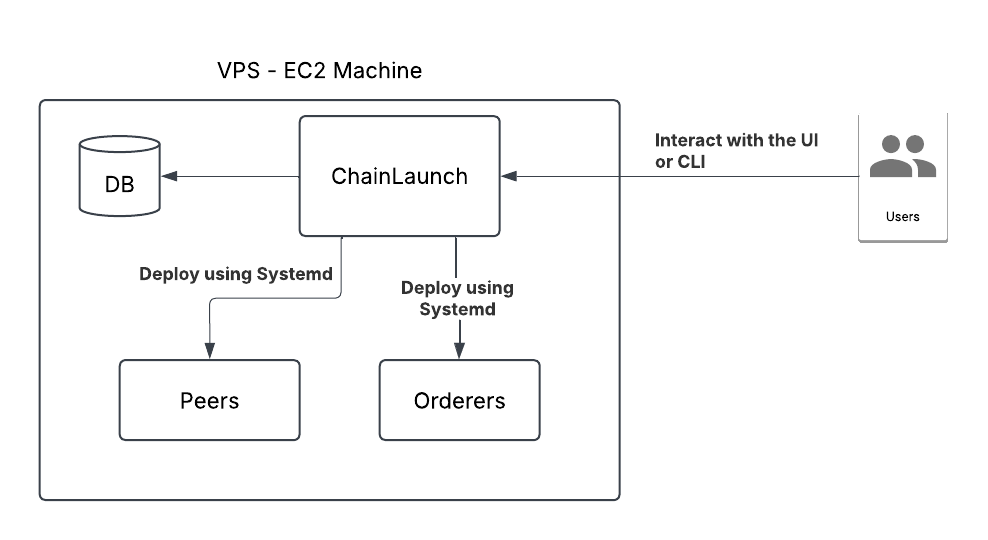
\includegraphics[width=0.95\textwidth, keepaspectratio]{Figures/Chainlaunch-architecture.png}
    \caption{Kiến trúc tổng thể của nền tảng Chainlaunch}
    \label{fig:chainlaunch-arch}
\end{figure}

\subsubsection{Công nghệ tầng Backend}

Tầng Backend đảm nhiệm toàn bộ logic nghiệp vụ, điều phối giao dịch tới mạng blockchain và quản lý dữ liệu ngoài chuỗi. Các công nghệ chủ đạo của tầng này được lựa chọn nhằm cân bằng giữa tính cấu trúc hóa của mã nguồn, độ an toàn kiểu dữ liệu và hiệu năng xử lý.

\begin{itemize}
    \item \textbf{NestJS -- Khung kiến trúc và mô hình quản trị logic:} NestJS chuẩn hóa kiến trúc máy chủ Node.js bằng cách áp dụng nghiêm ngặt mô hình \textit{Dependency Injection} (DI) và \textit{Inversion of Control} (IoC) thông qua cơ chế \textit{Decorators} và \textit{Metadata}. Nhờ đó, logic nghiệp vụ (Services) được phân tách rạch ròi khỏi logic điều phối (Controllers), giúp hệ thống đạt được tính bảo trì và khả năng kiểm thử cao. Việc tích hợp gói \pkg{@nestjs/microservices} còn cho phép trừu tượng hóa các tầng giao thức (TCP, gRPC, Redis Pub/Sub), tạo điều kiện chuyển đổi minh bạch từ mô hình đơn khối (Monolithic) sang phân tán (Microservices).

    \item \textbf{MongoDB và Prisma -- Tầng lưu trữ lai định kiểu:} MongoDB là cơ sở dữ liệu hướng tài liệu (document-oriented) phù hợp với các tập dữ liệu có cấu trúc biến đổi và yêu cầu mở rộng ngang (horizontal scaling); việc sử dụng định dạng \pkg{bson} giúp lưu trữ hiệu quả các cấu trúc phức tạp như cây Merkle. Prisma bổ khuyết nhược điểm thiếu cấu trúc của NoSQL bằng một bản đồ lược đồ (Schema) định nghĩa trước; engine của Prisma được viết bằng ngôn ngữ Rust, cung cấp khả năng tối ưu hóa truy vấn và ngăn chặn các lỗi runtime liên quan đến kiểu dữ liệu -- một yếu tố then chốt khi xử lý dữ liệu nhạy cảm như phiếu bầu.

    \item \textbf{Redis và cơ chế Cache -- Tối ưu hóa hiệu năng:} Hệ thống áp dụng mô hình lưu trữ đa tầng dựa trên công nghệ \pkg{cache-manager} và \pkg{@nestjs/cache-manager}, cho phép đồng bộ hóa trạng thái giữa các instance trong môi trường Microservices, giảm độ trễ mạng và tải trọng lên cơ sở dữ liệu chính. Redis đồng thời đóng vai trò bộ nhớ đệm trung tâm cho tác vụ giới hạn lưu lượng (Rate Limiting) thông qua \pkg{@nestjs/throttler}, giúp bảo vệ tài nguyên hệ thống trước các kịch bản tấn công khai thác hoặc quá tải truy cập nhờ tốc độ xử lý trên bộ nhớ RAM ở ngưỡng ms.
\end{itemize}

\subsubsection{Công nghệ tầng Website Frontend}

Tầng giao diện trình duyệt cung cấp môi trường tương tác cho quản trị viên và cử tri trên trình duyệt. Các công nghệ được lựa chọn nhằm tối ưu đồng thời trải nghiệm phát triển, hiệu năng tải trang và tính nhất quán về thiết kế.

\begin{itemize}
    \item \textbf{React -- Thư viện cốt lõi của tầng giao diện:} React là thư viện JavaScript được sử dụng để xây dựng giao diện người dùng theo mô hình lập trình khai báo (Declarative Programming) và kiến trúc thành phần tái sử dụng. Thông qua cơ chế đối chiếu (Reconciliation) trên DOM ảo (Virtual DOM), React xác định các thay đổi cần thiết và cập nhật chúng lên DOM thật một cách hiệu quả, từ đó giảm số lượng thao tác trực tiếp trên DOM và cải thiện hiệu năng hiển thị. Bên cạnh đó, mô hình luồng dữ liệu một chiều (Unidirectional Data Flow) cùng cơ chế truyền dữ liệu thông qua \pkg{props} giúp tăng tính minh bạch, khả năng dự đoán và khả năng bảo trì của ứng dụng.


    \item \textbf{Vite -- Công cụ xây dựng và tối ưu hóa chu kỳ phát triển:} Trong giai đoạn phát triển, Vite tận dụng tính năng ES Modules nguyên bản của trình duyệt cùng bộ biên dịch \textit{esbuild} (viết bằng ngôn ngữ Go) để loại bỏ giai đoạn đóng gói toàn bộ mã nguồn, nhờ đó giảm thời gian khởi động môi trường (Cold Start) xuống mức mili-giây. Trong giai đoạn biên dịch sản phẩm, Vite sử dụng \textit{Rollup} để thực thi các kỹ thuật phân tách mã động (Code-Splitting), loại bỏ mã thừa (Tree-Shaking) và tối ưu chiến lược tải trước tài nguyên, qua đó giữ kích thước tệp đầu ra ở mức tối thiểu và cải thiện trực tiếp các chỉ số Core Web Vitals.

    \item \textbf{Material UI và Emotion -- Hệ thống thiết kế và giải pháp CSS-in-JS:} Material UI (MUI) là thư viện giao diện người dùng cung cấp tập hợp các thành phần được xây dựng dựa trên ngôn ngữ thiết kế Material Design của Google. Kết hợp với giải pháp CSS-in-JS của Emotion (\pkg{@emotion/react} và \pkg{@emotion/styled}), MUI cho phép định nghĩa và quản lý phong cách trực tiếp trong thành phần giao diện, hạn chế xung đột giữa các lớp CSS và hỗ trợ tùy biến giao diện động trong quá trình thực thi. Bên cạnh đó, cơ chế quản lý giao diện tập trung giúp duy trì tính nhất quán về màu sắc, kiểu chữ và khoảng cách hiển thị trên toàn bộ hệ thống.

\end{itemize}

\subsubsection{Công nghệ tầng Mobile Frontend}

Tầng ứng dụng di động cho phép cử tri thực hiện bỏ phiếu trực tiếp trên thiết bị cá nhân. Để bảo đảm khả năng phát triển đa nền tảng từ một kho mã nguồn duy nhất cùng giao diện linh hoạt, tầng này được xây dựng dựa trên hai trụ cột công nghệ chính.

\begin{itemize}
    \item \textbf{Expo -- Nền tảng thực thi và quản lý vòng đời ứng dụng đa nền tảng:} Expo cung cấp giải pháp toàn diện để phát triển, biên dịch và vận hành ứng dụng trên iOS, Android và Web từ một kho mã nguồn duy nhất. Nền tảng này cung cấp các API đồng bộ giúp mã JavaScript tương tác trực tiếp với tính năng native của thiết bị (lưu trữ an toàn, định vị, camera) mà không cần can thiệp vào mã nguồn Java/Kotlin hay Objective-C/Swift. Cơ chế \textit{Expo Router} áp dụng mô hình định tuyến dựa trên tệp tin (File-based Routing), tự động hóa luồng điều hướng và tối ưu việc phân tách tài nguyên cũng như quản lý vòng đời của các màn hình.

    \item \textbf{React Native Reusables và Tailwind CSS -- Thư viện xây dựng UI:} Sự kết hợp này lấy cảm hứng trực tiếp từ mô hình \textit{Shadcn UI} trên nền tảng web, phân tách rạch ròi giữa logic vận hành và lớp trình bày của ứng dụng. Thay vì cung cấp các cấu phần đóng gói cứng nhắc, React Native Reusables (RNR) đưa cho nhà phát triển những component đơn giản (dựa trên \pkg{@rn-primitives}) đã được lập trình sẵn toàn bộ logic phức tạp bên dưới; nhà phát triển chỉ cần sao chép và tùy biến mã nguồn trực tiếp trong dự án, qua đó nắm quyền kiểm soát tuyệt đối và tránh phụ thuộc vào mã nguồn ẩn của bên thứ ba. Để hoàn thiện lớp vỏ ngoài, hệ thống sử dụng Tailwind CSS làm ngôn ngữ định kiểu theo hướng tiện ích (Utility-First): nhà phát triển chỉ cần gắn các \pkg{className} ngắn gọn để chỉ định màu sắc, khoảng cách và bố cục.
\end{itemize}

\input{Chapter-3/3.2-Tong-quan-mo-hinh-tin-cay}
\input{Chapter-3/3.3-EC-Schnorr-Blind-Multisignature}
\input{Chapter-3/3.4-JWT-hai-tang}
\input{Chapter-3/3.5-Quan-ly-session-Redis}
\input{Chapter-3/3.6-Hyperledger-Fabric}
\input{Chapter-3/3.7-Chainlaunch-Batch}
\input{Chapter-3/3.8-Merkle-Tree}
\subsection{Bảo mật tầng HTTP -- Helmet, CORS, Rate Limit và HTTPS}

Tầng HTTP là điểm tiếp xúc đầu tiên giữa cử tri và hệ thống, do đó các biện pháp phòng thủ tại tầng này được áp dụng đồng thời theo nhiều khía cạnh: \textit{tăng cường bảo mật tiêu đề HTTP} qua Helmet, giới hạn nguồn gốc qua CORS, giới hạn tần suất yêu cầu qua Rate Limiting, ngắt các yêu cầu vượt quá thời gian xử lý qua Timeout, và mã hóa truyền tải qua HTTPS.

\textbf{Helmet:} BFF và Reveal-Vote đều dùng thư viện \pkg{helmet} với cấu hình phân biệt theo môi trường (Hình~\ref{fig:helmet-config}). \textit{Content-Security-Policy} ở chế độ nghiêm ngặt với \pkg{default-src 'none'}, chỉ cho phép \pkg{connect-src 'self'} và buộc nâng cấp HTTP sang HTTPS. Các tiêu đề khác như \pkg{X-Frame-Options}, \pkg{X-Content-Type-Options}, \pkg{Referrer-Policy}, \pkg{Strict-Transport-Security}, \pkg{Cross-Origin-Opener-Policy} đều được bật mặc định.

\begin{figure}[H]
    \centering
    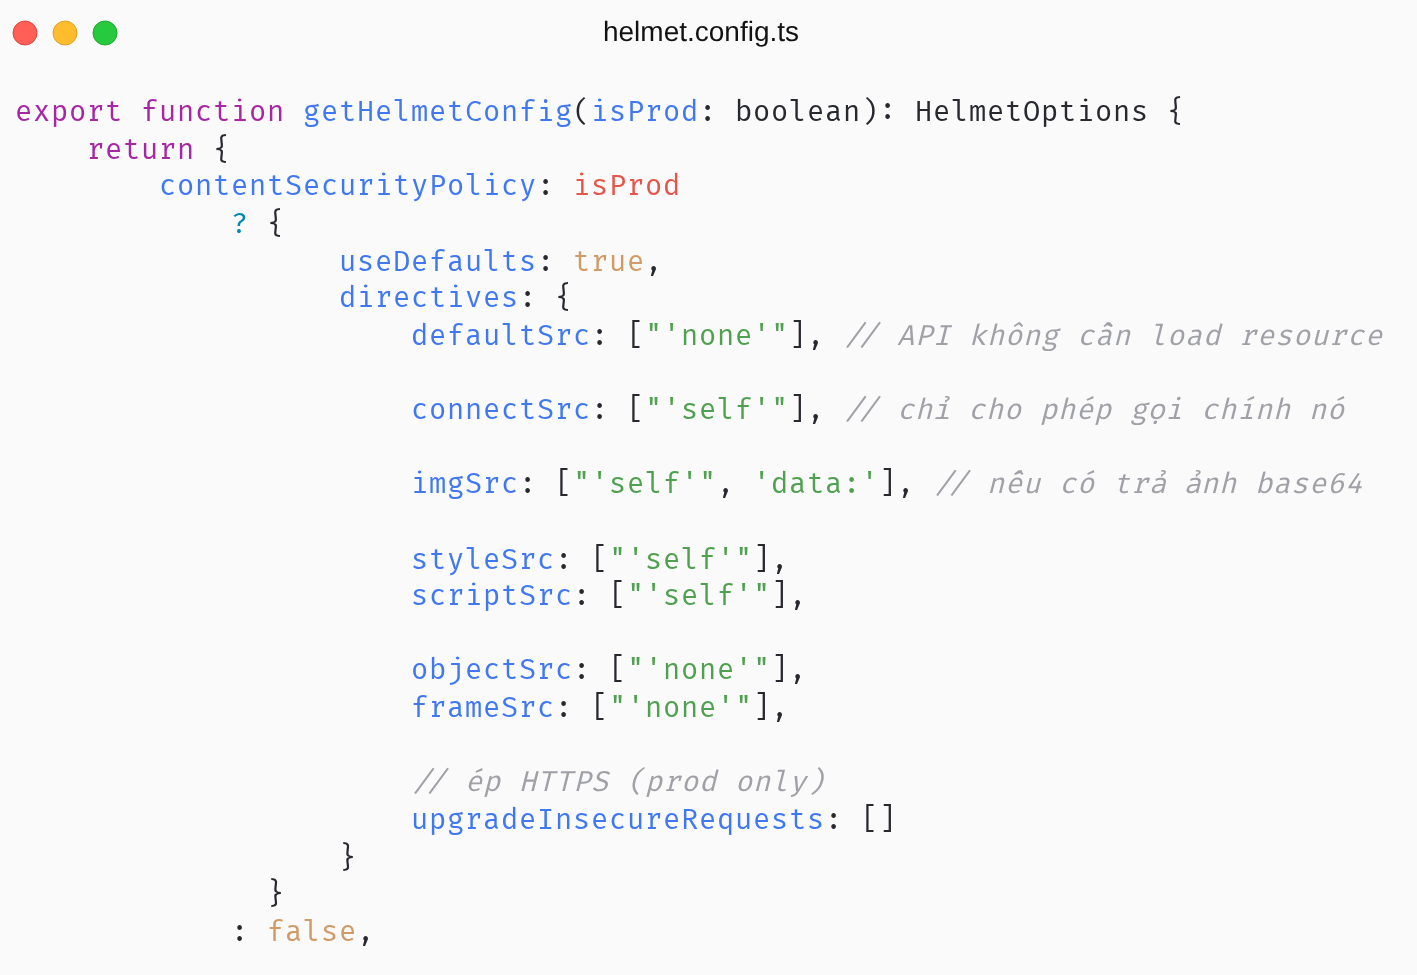
\includegraphics[width=0.85\textwidth, keepaspectratio]{Figures/code/helmet-config.png}
    \caption{Cấu hình Helmet cho môi trường sản xuất}
    \label{fig:helmet-config}
\end{figure}

\textbf{CORS:} Tiêu đề \pkg{Access-Control-Allow-Origin} chỉ chấp nhận các tên miền nằm trong biến môi trường \pkg{CORS\_ORIGINS}. Phương thức được phép giới hạn ở \pkg{GET}, \pkg{POST}, \pkg{PUT}, \pkg{PATCH}, \pkg{DELETE}, \pkg{OPTIONS}, kèm \pkg{credentials} để cookie phiên hợp lệ cho các tên miền tin cậy. Cấu hình này ngăn các trang web bên ngoài gọi API qua \pkg{XMLHttpRequest} hay \pkg{fetch} và đảm nhận một phần vai trò chống CSRF.

\textbf{Rate Limiting:} \pkg{HttpThrottlerGuard} giới hạn 100 yêu cầu mỗi IP trong mỗi 60 giây.

\textbf{Request Timeout:} \pkg{TimeoutInterceptor} áp dụng toán tử \pkg{timeout(5000)} của RxJS cho mọi yêu cầu -- sau 5 giây hệ thống trả về \pkg{408 Request Timeout} thay vì giữ kết nối vô thời hạn. Cơ chế này quan trọng khi peer Fabric phản hồi chậm: yêu cầu của cử tri không bị treo, cho phép họ thử lại thay vì chờ đợi không xác định.

\textbf{HTTPS cho BFF và Reveal-Vote:} Hai dịch vụ đều được phục vụ qua HTTPS. Hệ thống áp dụng mô hình \textit{TLS termination at edge}: một reverse proxy Cloudflare đứng trước, đảm nhận giải mã TLS rồi chuyển tiếp yêu cầu HTTP đến backend trong mạng nội bộ tin cậy. Cách triển khai này tận dụng phần cứng tăng tốc TLS của reverse proxy và giúp việc luân chuyển chứng chỉ trở nên đơn giản -- chỉ phải cập nhật tại một điểm. Trường hợp triển khai trên một máy chủ duy nhất, NestJS hỗ trợ bật HTTPS trực tiếp như sau:

\begin{figure}[H]
    \centering
    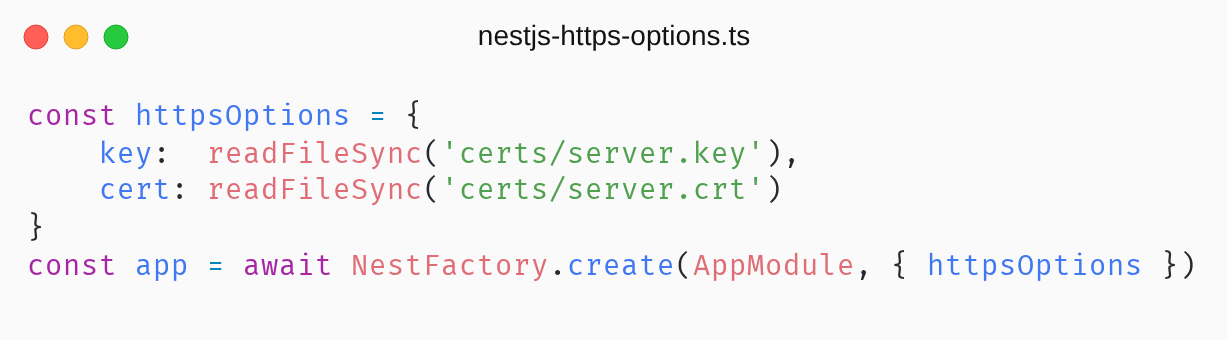
\includegraphics[width=0.70\textwidth, keepaspectratio]{Figures/code/nestjs-https-options.png}
    \caption{Khởi tạo NestJS với httpsOptions để bật HTTPS trực tiếp}
    \label{fig:nestjs-https-options}
\end{figure}

\subsection{Giao tiếp nội bộ -- TCP NestJS, mTLS và xác thực dữ liệu đầu vào}

Các dịch vụ nội bộ của hệ thống giao tiếp với nhau qua \textbf{NestJS TCP transport} thay vì REST HTTP. Cách làm này loại bỏ tầng parser HTTP, giảm độ trễ trung bình từ 5--15 ms xuống còn 1--3 ms cho mỗi vòng gọi, và quan trọng hơn -- các dịch vụ ngoài BFF và Reveal-Vote không cần mở cổng HTTP, do đó không trực tiếp tiếp xúc với mạng bên ngoài. Sơ đồ giao tiếp tổng thể được minh họa trong Hình~\ref{fig:internal-services}.

\textbf{mTLS cho kênh TCP giữa các microservice:} Do các microservice có thể được triển khai trên các máy chủ khác nhau và giao tiếp thông qua hạ tầng mạng không hoàn toàn tin cậy, hệ thống sử dụng \textit{mutual TLS} (mTLS) để mã hóa dữ liệu truyền tải và xác thực hai chiều danh tính dịch vụ. Nhờ đó, chỉ những dịch vụ sở hữu chứng chỉ hợp lệ mới có thể tham gia trao đổi dữ liệu. Cấu hình microservice của NestJS được khởi tạo với \pkg{tlsOptions}:

\begin{figure}[H]
    \centering
    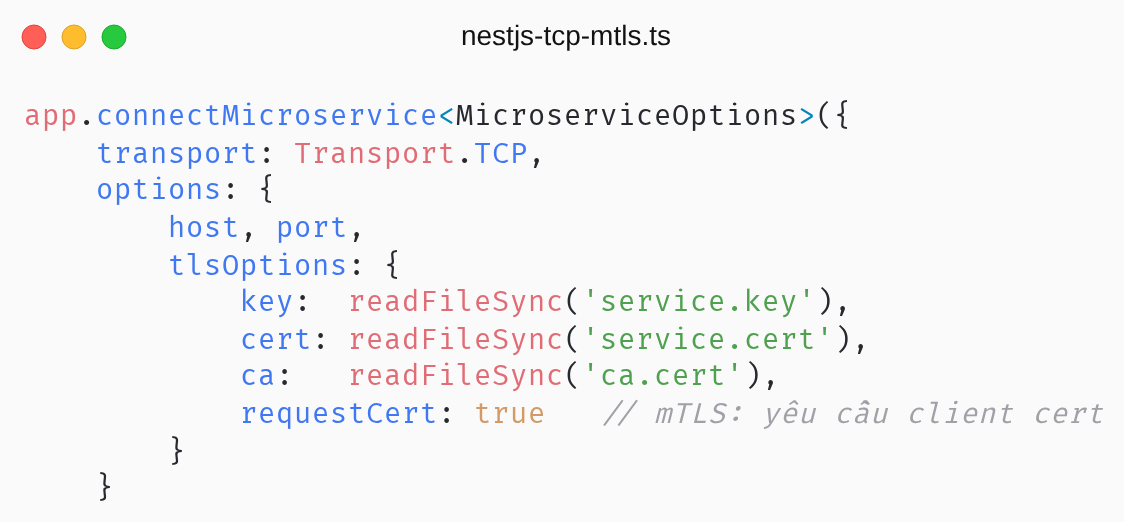
\includegraphics[width=0.75\textwidth, keepaspectratio]{Figures/code/nestjs-tcp-mtls.png}
    \caption{Cấu hình mTLS cho NestJS TCP microservice với tlsOptions}
    \label{fig:nestjs-tcp-mtls}
\end{figure}

\textbf{Xác thực dữ liệu đầu vào:} Mọi yêu cầu vào hệ thống -- cả từ trình duyệt qua HTTP đến BFF lẫn từ microservice qua kênh TCP -- đều được kiểm chứng tự động qua \pkg{ValidationPipe} toàn cục. Lớp DTO khai báo các ràng buộc dưới dạng decorator của \pkg{class-validator}: \pkg{@IsDefined}, \pkg{@IsString},... Ví dụ điển hình là \pkg{SignInDto} và \pkg{RefreshTokenDto} trong Hình~\ref{fig:class-validator-dto}.

\begin{figure}[H]
    \centering
    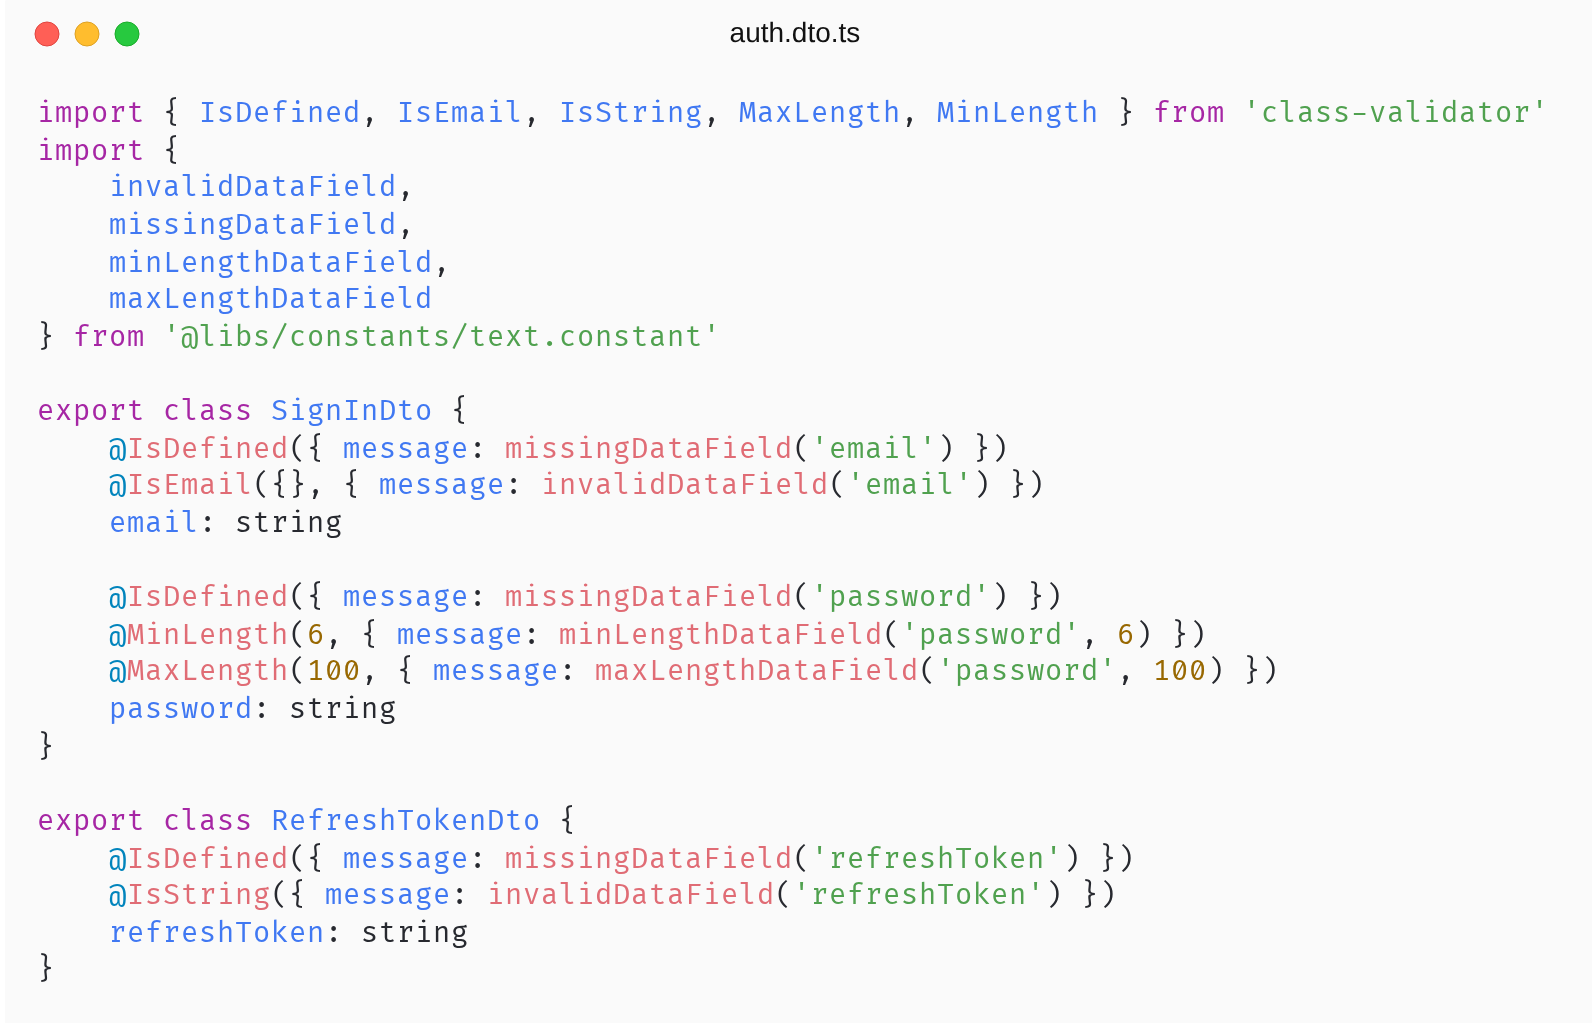
\includegraphics[width=0.85\textwidth, keepaspectratio]{Figures/code/class-validator-dto.png}
    \caption{DTO xác thực dữ liệu vào bằng decorator của class-validator}
    \label{fig:class-validator-dto}
\end{figure}

\input{Chapter-3/3.11-AES-256-GCM}
\subsection{Tối ưu hiệu năng hệ thống}

Một số kỹ thuật tối ưu hiệu năng được áp dụng nhằm giữ độ trễ ở mức chấp nhận được dưới tải bầu cử đỉnh -- khi hàng nghìn cử tri có thể đồng thời bỏ phiếu trong cùng một khoảng thời gian ngắn.

\textbf{MongoDB Replica Set và Prisma transaction:} Cụm MongoDB được khởi tạo với \pkg{--replSet rs0}, là điều kiện bắt buộc để Prisma sử dụng \pkg{\$transaction} với nhiều thao tác ACID. Hệ thống tuân thủ \textit{kiểm tra hợp lệ ngoài giao dịch, chỉ ghi (commit) trong giao dịch}: các thao tác đọc và side-effect nặng (gọi Fabric mất 2--3 giây) được thực hiện \textbf{ngoài} giao dịch; giao dịch chỉ chứa hai bước \textit{re-validate} (chống xung đột đồng thời) và \textit{ghi}. Nhờ đó thời gian giữ khóa của giao dịch ngắn, thông lượng tăng đáng kể so với cách bao bọc toàn bộ luồng nghiệp vụ.

\textbf{Cache phản hồi HTTP:} \pkg{HttpCacheInterceptor} đệm phản hồi của các yêu cầu \pkg{GET} vào Redis. Các endpoint danh sách bầu cử công khai và xem chi tiết ứng viên hưởng lợi nhiều nhất từ cơ chế này vì chúng có tải đọc cao và dữ liệu thay đổi ít.

\textbf{Chiến lược chỉ mục MongoDB:} Các bảng chính được phủ chỉ mục để mọi thao tác đọc theo dõi được $O(\log N)$ hoặc $O(1)$ thay vì quét tuần tự. Bảng~\ref{tab:mongo-index} liệt kê các chỉ mục then chốt.

\begin{table}[H]
\centering
\caption{Chiến lược chỉ mục các bảng chính trong MongoDB}
\label{tab:mongo-index}
\begin{tabularx}{\textwidth}{|L{0.2}|L{0.4}|L{0.4}|}
\hline
\textbf{Bảng} & \textbf{Chỉ mục} & \textbf{Mục đích} \\
\hline
\pkg{elections} & \pkg{(status, startDate, endDate)} & Lọc bầu cử theo trạng thái và thời gian \\
\hline
\pkg{election\_voters} & \pkg{unique(electionId, voterId)} & Tra cứu O(1) và loại bỏ phần tử trùng lặp \\
\hline
\pkg{votes} & \pkg{unique(electionId, voterId)} & Chống bỏ phiếu hai lần \\
 & \pkg{unique(electionId, blindedCommitment)} & Chống nộp commitment trùng \\
 & \pkg{(electionId, createdAt)} & Lấy theo thứ tự cho cây Merkle \\
\hline
\pkg{revealed\_votes} & \pkg{unique(electionId, revealKey)} & Chống phát lại reveal \\
 & \pkg{(electionId, candidateId)} & Tổng hợp kết quả theo ứng viên \\
\hline
\end{tabularx}
\end{table}

\textbf{Truy vấn song song:} Những tác vụ độc lập không phụ thuộc lẫn nhau được thực thi đồng thời bằng \pkg{Promise.all}. Ví dụ, khi hiển thị kết quả bầu cử, hệ thống đồng thời lấy dữ liệu từ MongoDB, Coordinator Service và Hyperledger Fabric thay vì chờ từng truy vấn hoàn thành tuần tự. Nhờ đó, thời gian phản hồi chỉ phụ thuộc vào truy vấn chậm nhất, giúp giảm đáng kể độ trễ khi tải dữ liệu.

\subsection{Nhất quán dữ liệu giữa blockchain và MongoDB}

Mỗi thao tác nghiệp vụ quan trọng của hệ thống đều phải ghi đồng thời lên hai hệ lưu trữ tách biệt: sổ cái Hyperledger Fabric và cơ sở dữ liệu MongoDB. Hai lần ghi này không thể bọc chung trong một giao dịch nguyên tử (\textit{atomic}). Nếu ghi chuỗi khối trước rồi ghi cơ sở dữ liệu sau (\textit{chain-first}), một lỗi xảy ra ở bước ghi cơ sở dữ liệu — \textbf{sau khi} chuỗi khối đã ghi nhận thành công — sẽ làm hai bên lệch nhau; và vì sổ cái là bất biến nên không thể hoàn tác. Bảng~\ref{tab:dual-write} liệt kê ba điểm ghi kép cùng hậu quả khi lệch theo hướng \textit{chain-first}.

\begin{table}[H]
\centering
\caption{Ba điểm ghi kép và hậu quả khi lệch dữ liệu theo hướng chain-first}
\label{tab:dual-write}
\begin{tabularx}{\textwidth}{|L{0.32}|L{0.68}|}
\hline
\textbf{Thao tác} & \textbf{Hậu quả khi chuỗi khối thành công nhưng cơ sở dữ liệu lỗi} \\
\hline
\pkg{SubmitVote} & Chuỗi khối có phiếu, cơ sở dữ liệu thiếu $\rightarrow$ số phiếu hai bên lệch $\rightarrow$ lệnh \pkg{CommitMerkleRoot} bị từ chối khi đóng cuộc bầu cử. \\
\hline
\pkg{CommitMerkleRoot} & Chuỗi khối đã đóng, cơ sở dữ liệu còn \pkg{ACTIVE} $\rightarrow$ thử lại bị từ chối (do tính idempotent) $\rightarrow$ cuộc bầu cử bị kẹt. \\
\hline
\pkg{RevealVoteCompact} & Chuỗi khối đã dùng \pkg{revealKey}, cơ sở dữ liệu thiếu $\rightarrow$ cử tri thử lại bị báo ``revealKey đã dùng'' $\rightarrow$ không thể tiết lộ lại. \\
\hline
\end{tabularx}
\end{table}

\subsubsection{Giải pháp 1 --- Ghi cơ sở dữ liệu trước kèm trạng thái trung gian}

Hai thao tác \pkg{SubmitVote} và đóng cuộc bầu cử áp dụng mô hình \textit{Write-DB-First}: ghi cơ sở dữ liệu ở một trạng thái trung gian \textbf{trước}, rồi mới gọi chuỗi khối, sau đó xác nhận lại cơ sở dữ liệu. Trình tự gồm bốn bước:

\begin{itemize}
    \item \textbf{Bước 1 --- Ghi trạng thái trung gian:} ghi bản ghi với trạng thái \pkg{Vote.status = PENDING\_CHAIN} (đối với phiếu) hoặc \pkg{Election.status = CLOSING} (đối với đóng cuộc bầu cử), trường \pkg{blockchainRef} để trống. Vì cơ sở dữ liệu được ghi trước, ràng buộc duy nhất \pkg{(electionId, voterId)} chặn bỏ phiếu trùng ngay tại bước này — trước cả khi chạm tới chuỗi khối; riêng \pkg{CLOSING} còn đóng vai trò khóa chống đóng cuộc bầu cử đồng thời.

    \item \textbf{Bước 2 --- Gọi chuỗi khối:} thực thi giao dịch \textit{invoke} tương ứng.

    \item \textbf{Bước 3 --- Chuỗi khối thành công:} xác nhận cơ sở dữ liệu, chuyển trạng thái sang \pkg{CONFIRMED} (hoặc \pkg{CLOSED}) và ghi \pkg{blockchainRef} bằng mã giao dịch trả về.

    \item \textbf{Bước 4 --- Chuỗi khối báo lỗi:} truy vấn lại chuỗi khối (\pkg{GetVote} hoặc \pkg{GetMerkleRoot}) để phân định, vì chuỗi khối là \textbf{nguồn sự thật}: nếu dữ liệu \textit{đã} có trên chuỗi khối thì xác nhận cơ sở dữ liệu và phục hồi mã giao dịch từ kết quả truy vấn; nếu \textit{chưa} có thì hoàn tác cơ sở dữ liệu (xóa phiếu \pkg{PENDING\_CHAIN} hoặc đưa cuộc bầu cử về \pkg{ACTIVE}) rồi ném lỗi để người dùng thử lại.
\end{itemize}

Hình~\ref{fig:submit-vote-write-db-first} trình bày hiện thực của mô hình này trong thao tác nộp phiếu.

\begin{figure}[H]
    \centering
    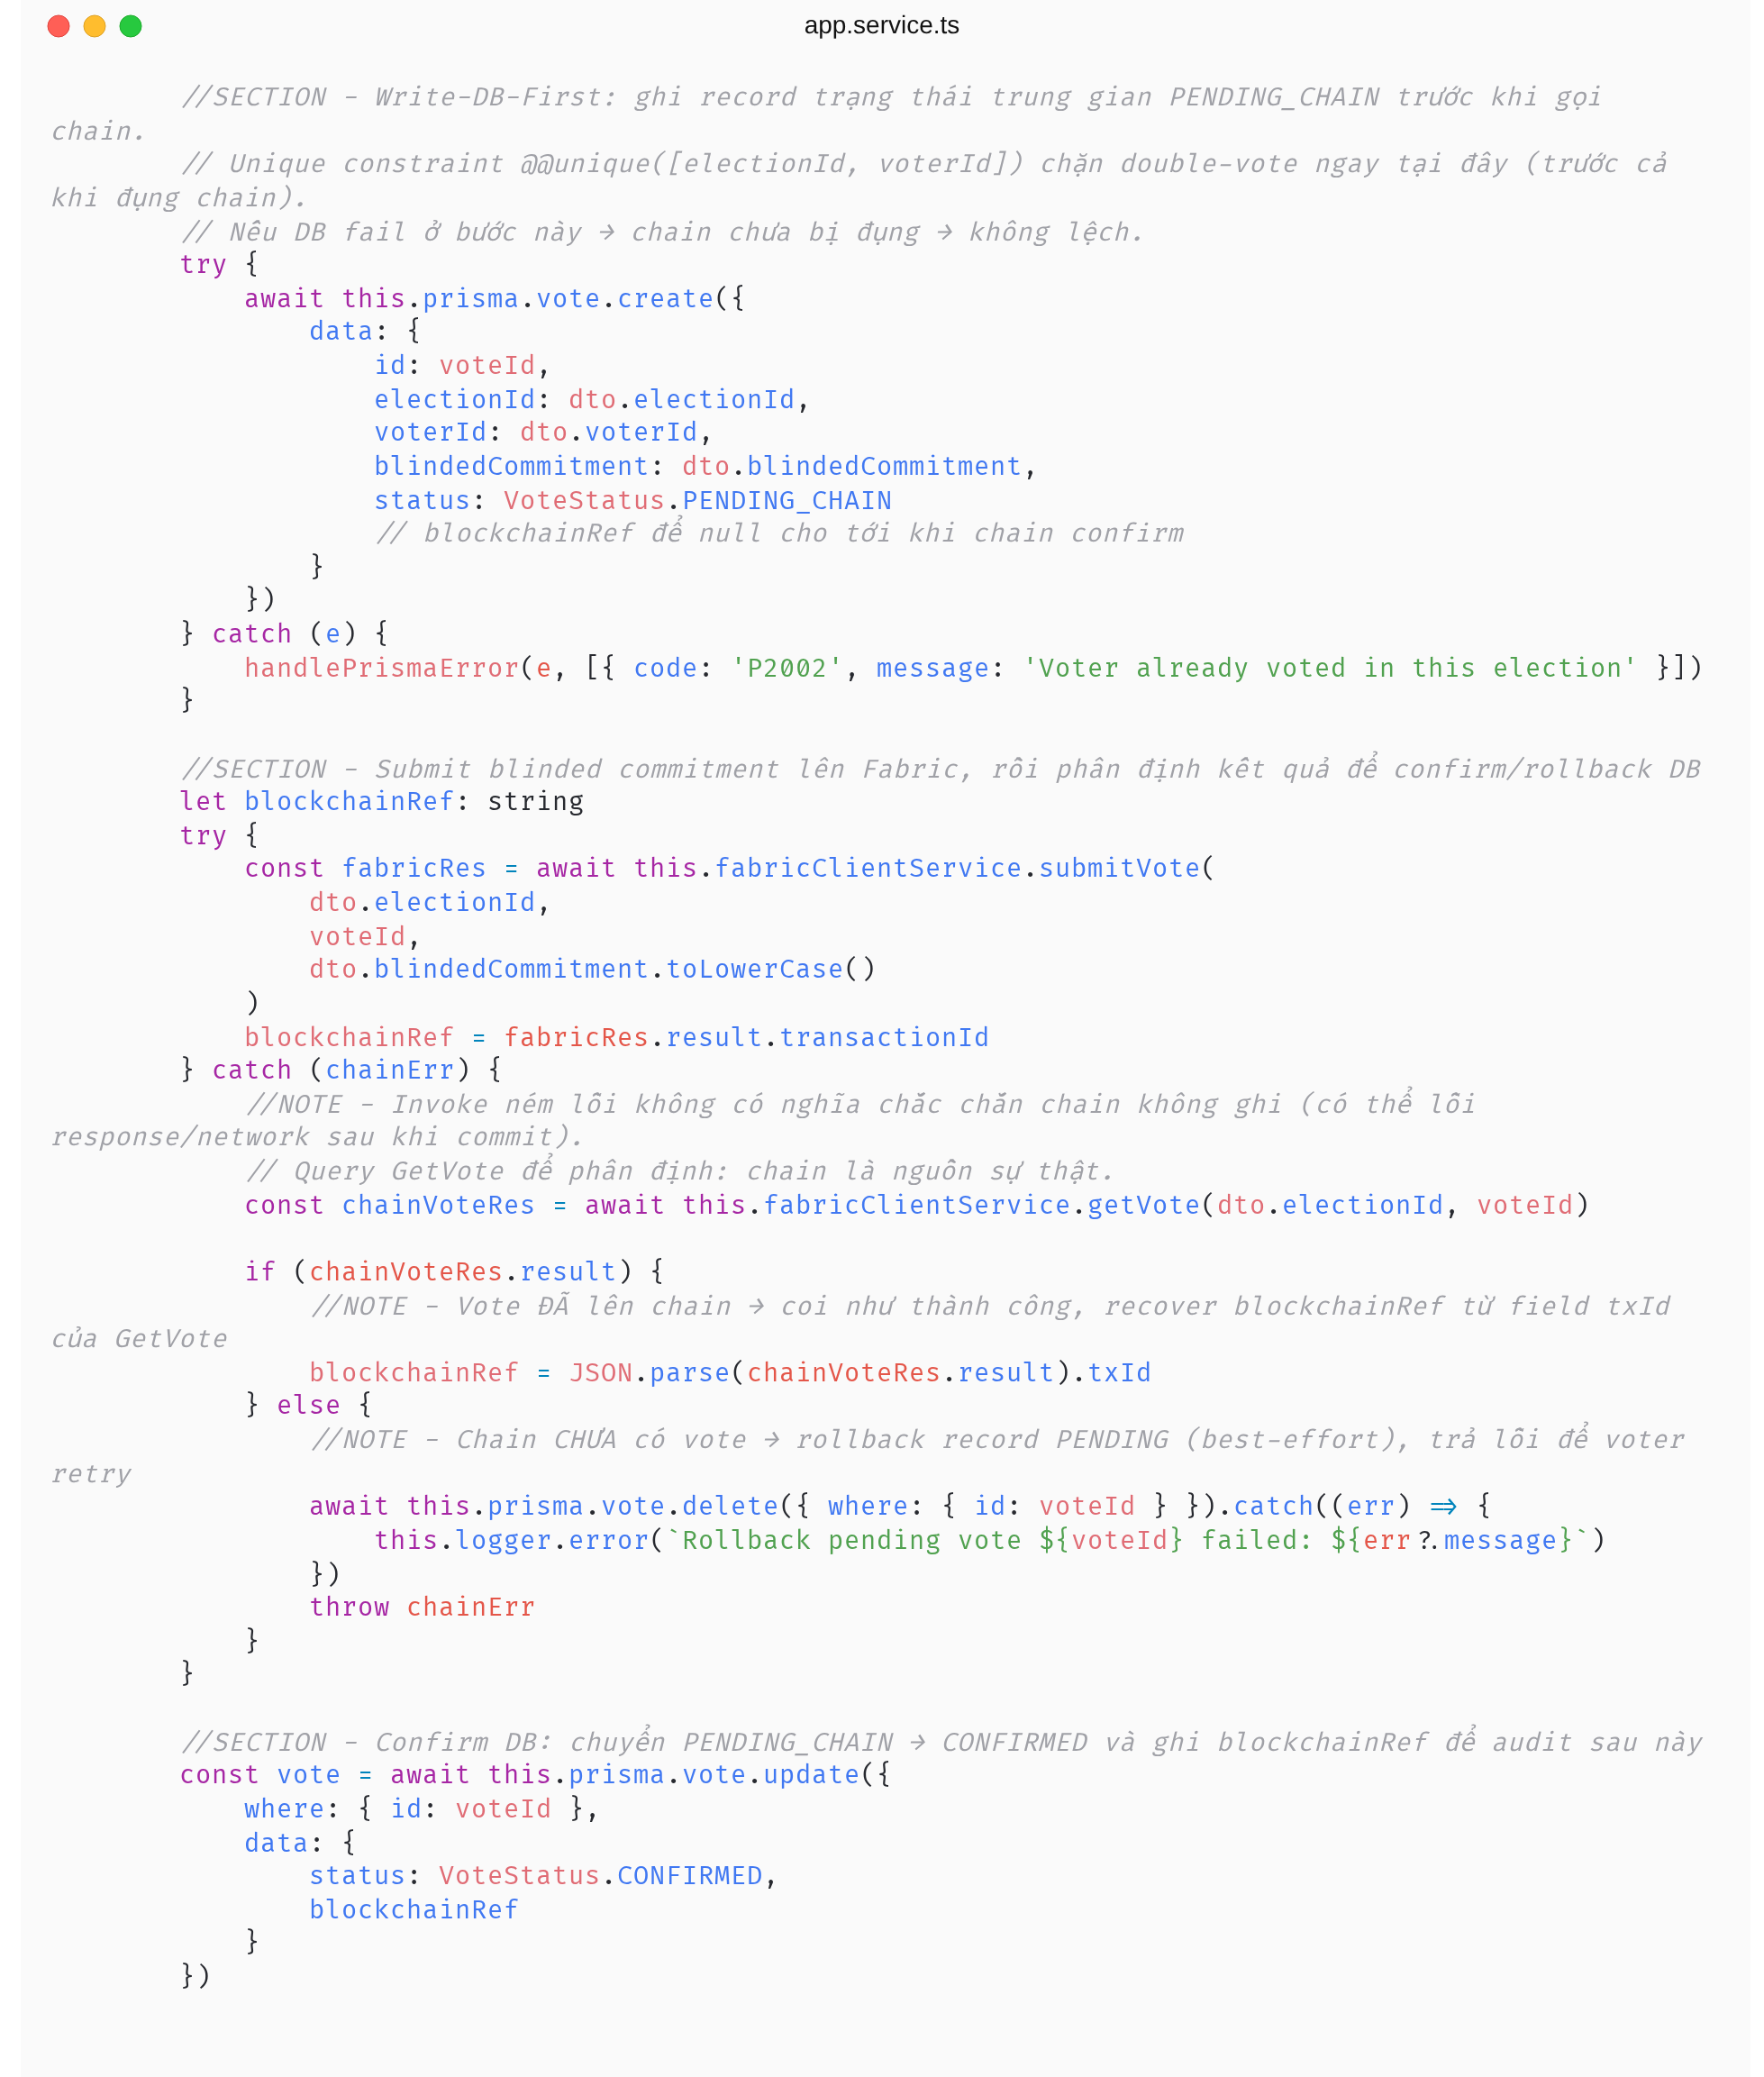
\includegraphics[width=\textwidth, keepaspectratio]{Figures/code/submit-vote-write-db-first.png}
    \caption{Mô hình Write-DB-First trong thao tác nộp phiếu \pkg{submitBlindedCommitment}}
    \label{fig:submit-vote-write-db-first}
\end{figure}

\subsubsection{Giải pháp 2 --- Giữ chain-first kèm tự phục hồi khi thử lại}

Thao tác \pkg{RevealVoteCompact} không đổi thứ tự ghi (vẫn chuỗi khối trước, cơ sở dữ liệu sau) vì \pkg{revealKey} là khóa idempotent tự nhiên trên chuỗi khối. Khi lệnh \textit{invoke} báo lỗi, hệ thống truy vấn \pkg{GetUsedReveal}: nếu chuỗi khối \textit{chưa} có \pkg{revealKey} thì đây là lỗi thật, ném tiếp; nếu chuỗi khối \textit{đã} có (và danh sách ứng viên khớp) thì coi là thử lại sau lỗi một phần, hệ thống ghi lại bản ghi cơ sở dữ liệu với \pkg{blockchainRef} để trống. Ràng buộc duy nhất \pkg{(electionId, revealKey)} vẫn ném lỗi nếu cơ sở dữ liệu đã có bản ghi, do đó tấn công phát lại thật vẫn bị chặn — chỉ phục hồi khi cơ sở dữ liệu còn trống.

\subsubsection{Tiến trình đồng bộ nền (Reconciler)}

Hai giải pháp trên xử lý lỗi trong luồng đồng bộ của yêu cầu. Trường hợp tiến trình \textit{sập} giữa bước gọi chuỗi khối và bước xác nhận sẽ để lại bản ghi kẹt ở trạng thái trung gian. Một tiến trình đồng bộ nền (\textit{reconciler}) chạy theo lịch \pkg{@Cron} của \pkg{@nestjs/schedule} đảm nhiệm việc dọn dẹp: định kỳ quét các bản ghi kẹt \textbf{cũ hơn} một ngưỡng thời gian (tránh tranh chấp với yêu cầu đang chạy), có cờ chống chồng lấn chu kỳ:

\begin{itemize}
    \item Phiếu còn \pkg{PENDING\_CHAIN}: truy vấn \pkg{GetVote} --- nếu có trên chuỗi khối thì chuyển \pkg{CONFIRMED}, nếu không thì xóa bản ghi.
    \item Cuộc bầu cử còn \pkg{CLOSING}: truy vấn \pkg{GetMerkleRoot} --- nếu đã cố định thì chuyển \pkg{CLOSED} và phục hồi mã giao dịch, nếu không thì giữ nguyên chờ quản trị viên thử lại.
\end{itemize}

\begin{figure}[H]
    \centering
    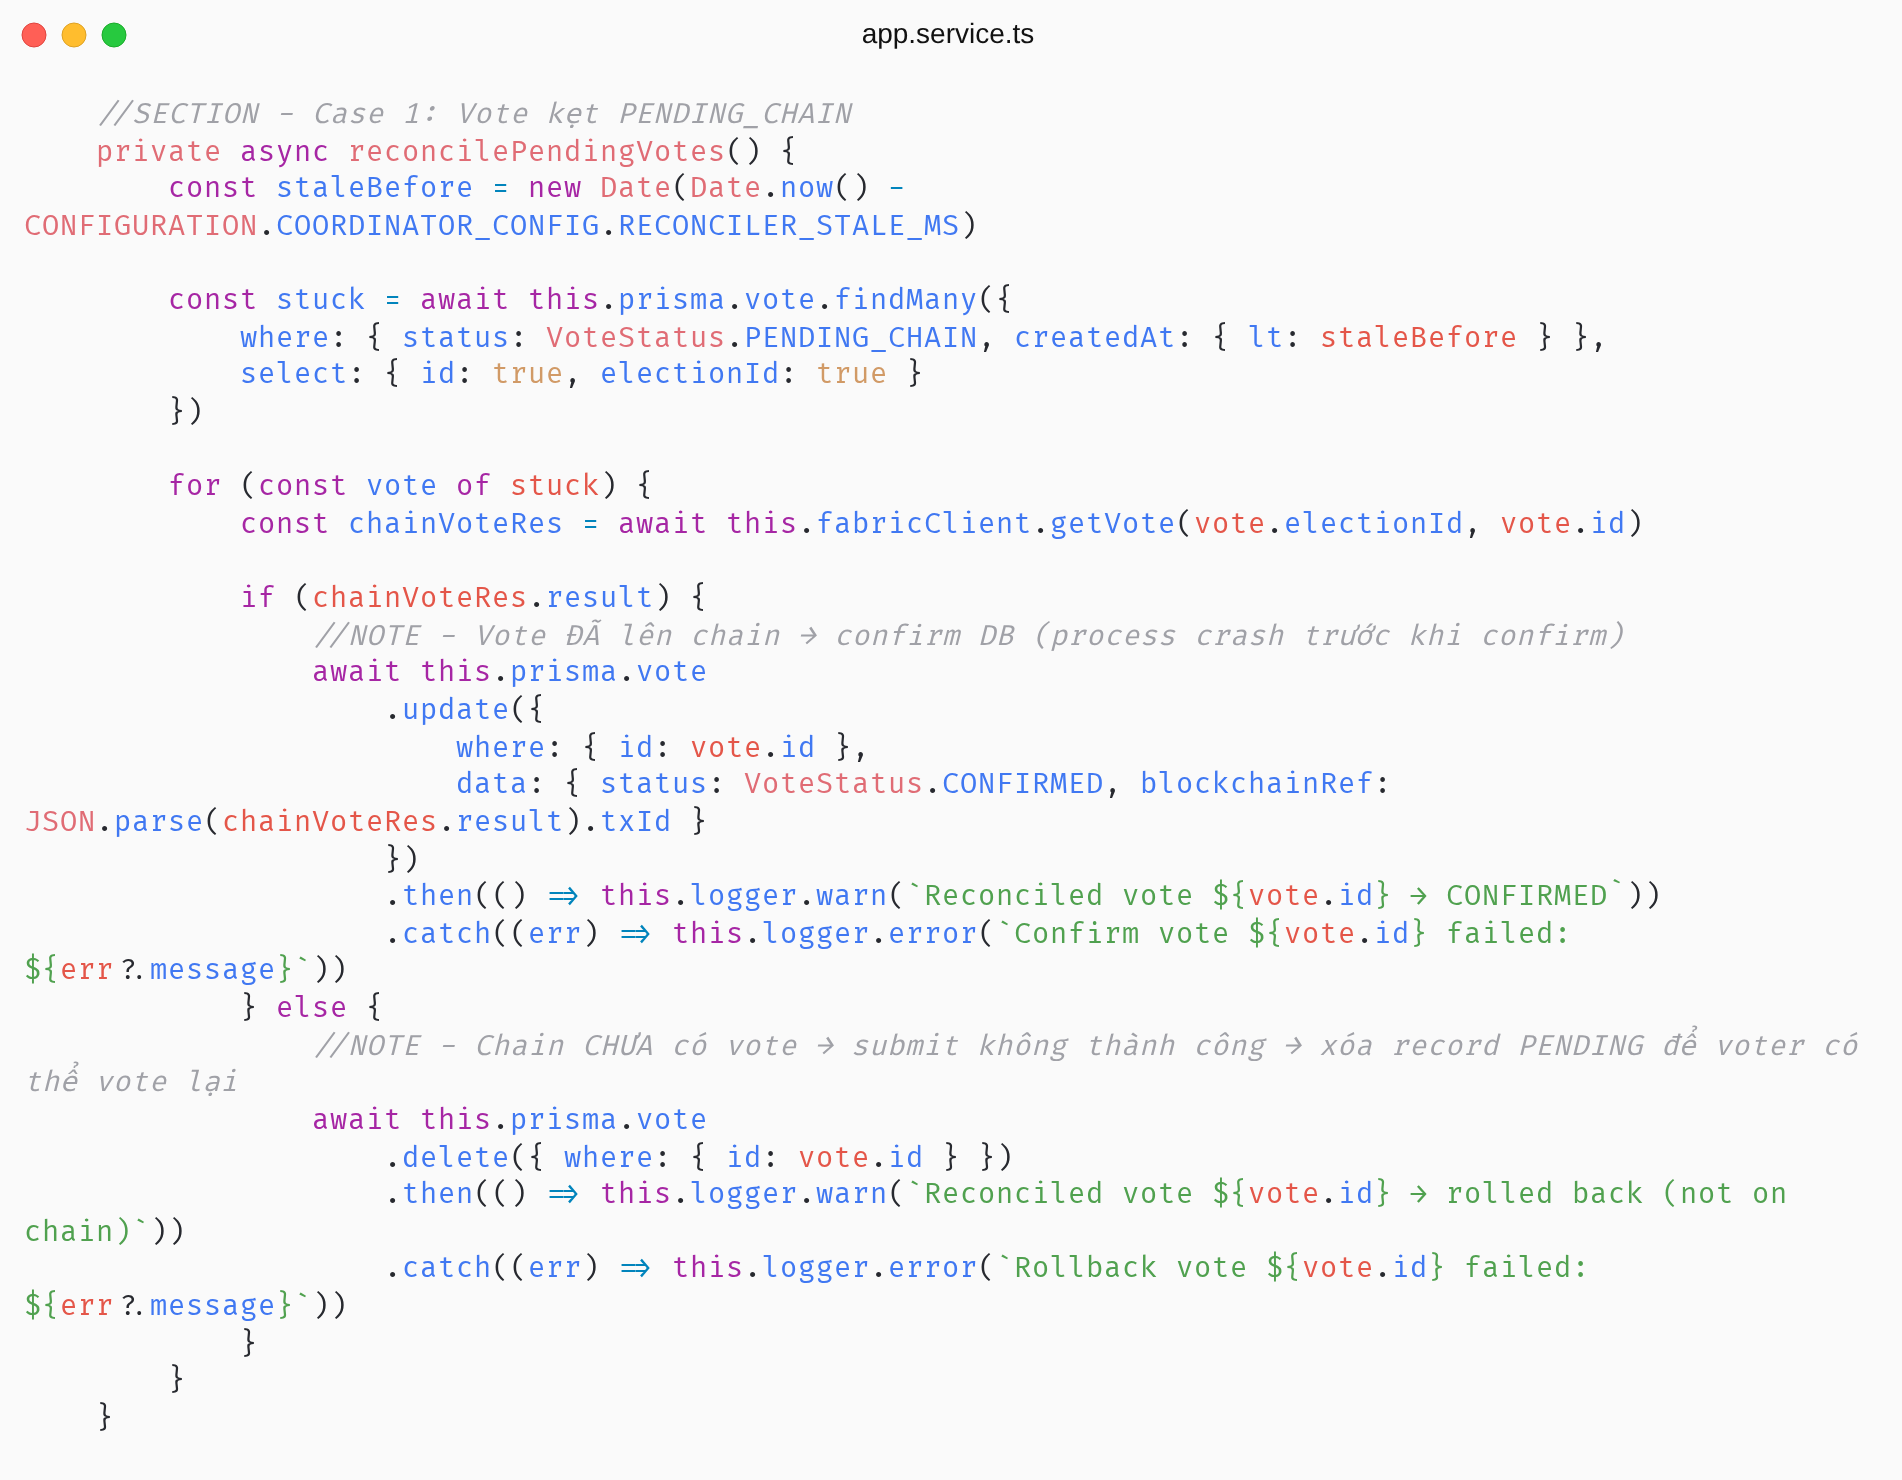
\includegraphics[width=\textwidth, keepaspectratio]{Figures/code/reconciler-pending-vote.png}
    \caption{Tiến trình đồng bộ nền đối chiếu phiếu \pkg{PENDING\_CHAIN} với chuỗi khối}
    \label{fig:reconciler-pending-vote}
\end{figure}

\subsubsection{Hệ quả về bất biến đọc dữ liệu}

Do chuỗi khối là nguồn sự thật, một phiếu chỉ được coi là hợp lệ khi đã \pkg{CONFIRMED}. Vì vậy mọi hàm đọc phiếu (đếm phiếu, dựng cây Merkle khi đóng, lọc danh sách phiếu) đều \textbf{mặc định lọc} \pkg{status = CONFIRMED} để khớp đúng tập phiếu thực sự có trên chuỗi khối. Hai ngoại lệ được giữ \textit{không phụ thuộc trạng thái} một cách có chủ đích: kiểm tra bỏ phiếu trùng khi khởi tạo phiên (phiếu \pkg{PENDING\_CHAIN} vẫn phải tính là ``đã bỏ phiếu'' để giữ chỗ) và thao tác xác minh phiếu phục vụ điều tra (cần thấy cả phiếu \pkg{PENDING\_CHAIN} để phát hiện lệch dữ liệu). Đây là mô hình \textit{nhất quán cuối} (\textit{eventual consistency}): trong khoảng chuỗi khối tạm thời không phản hồi, một phiếu có thể nằm ở \pkg{PENDING\_CHAIN} cho tới khi tiến trình đồng bộ nền đưa nó về trạng thái cuối cùng.

\subsection{Sao lưu và khôi phục khóa bí mật phiếu}

Sau khi bỏ phiếu, cử tri giữ một tập \textit{khóa bí mật phiếu} ngay trên thiết bị di động — gồm các hệ số làm mù $(\alpha, \beta)$, hai thành phần chữ ký $(h, s')$ và danh sách ứng viên đã chọn — được lưu trong kho lưu trữ an toàn (\textit{Secure Store}) của hệ điều hành. Tập khóa này là điều kiện bắt buộc để cử tri tiết lộ phiếu và tự xác minh phiếu về sau; mất thiết bị đồng nghĩa mất vĩnh viễn khả năng đó. Hệ thống vì vậy cung cấp cơ chế sao lưu và khôi phục các khóa này lên máy chủ mà vẫn không làm suy giảm tính bí mật, theo mô hình \textit{zero-knowledge}.

\subsubsection{Lớp mã hóa phía máy khách (zero-knowledge)}

Toàn bộ việc mã hóa diễn ra trên thiết bị, trước khi bất kỳ dữ liệu nào rời khỏi máy khách. Cử tri đặt một mã PIN; ứng dụng dẫn xuất khóa đối xứng 256-bit từ mã PIN bằng hàm \pkg{PBKDF2-SHA256} với $100{,}000$ vòng lặp và một salt ngẫu nhiên, sau đó mã hóa tập khóa bằng \pkg{AES-256-GCM}. Kết quả là một gói dữ liệu (\textit{envelope}) JSON chứa tham số dẫn xuất khóa (thuật toán, số vòng, salt) và phần bản mã (vector khởi tạo, bản mã kèm thẻ xác thực). Vì máy chủ \textbf{không bao giờ nhận mã PIN}, máy chủ không thể dẫn lại khóa nên không thể giải lớp mã hóa này. Số vòng lặp lớn của PBKDF2 làm chậm đáng kể tấn công dò mã PIN theo kiểu vét cạn. Hình~\ref{fig:backup-derive-key} trình bày hàm dẫn xuất khóa và mã hóa gói envelope.

\begin{figure}[H]
    \centering
    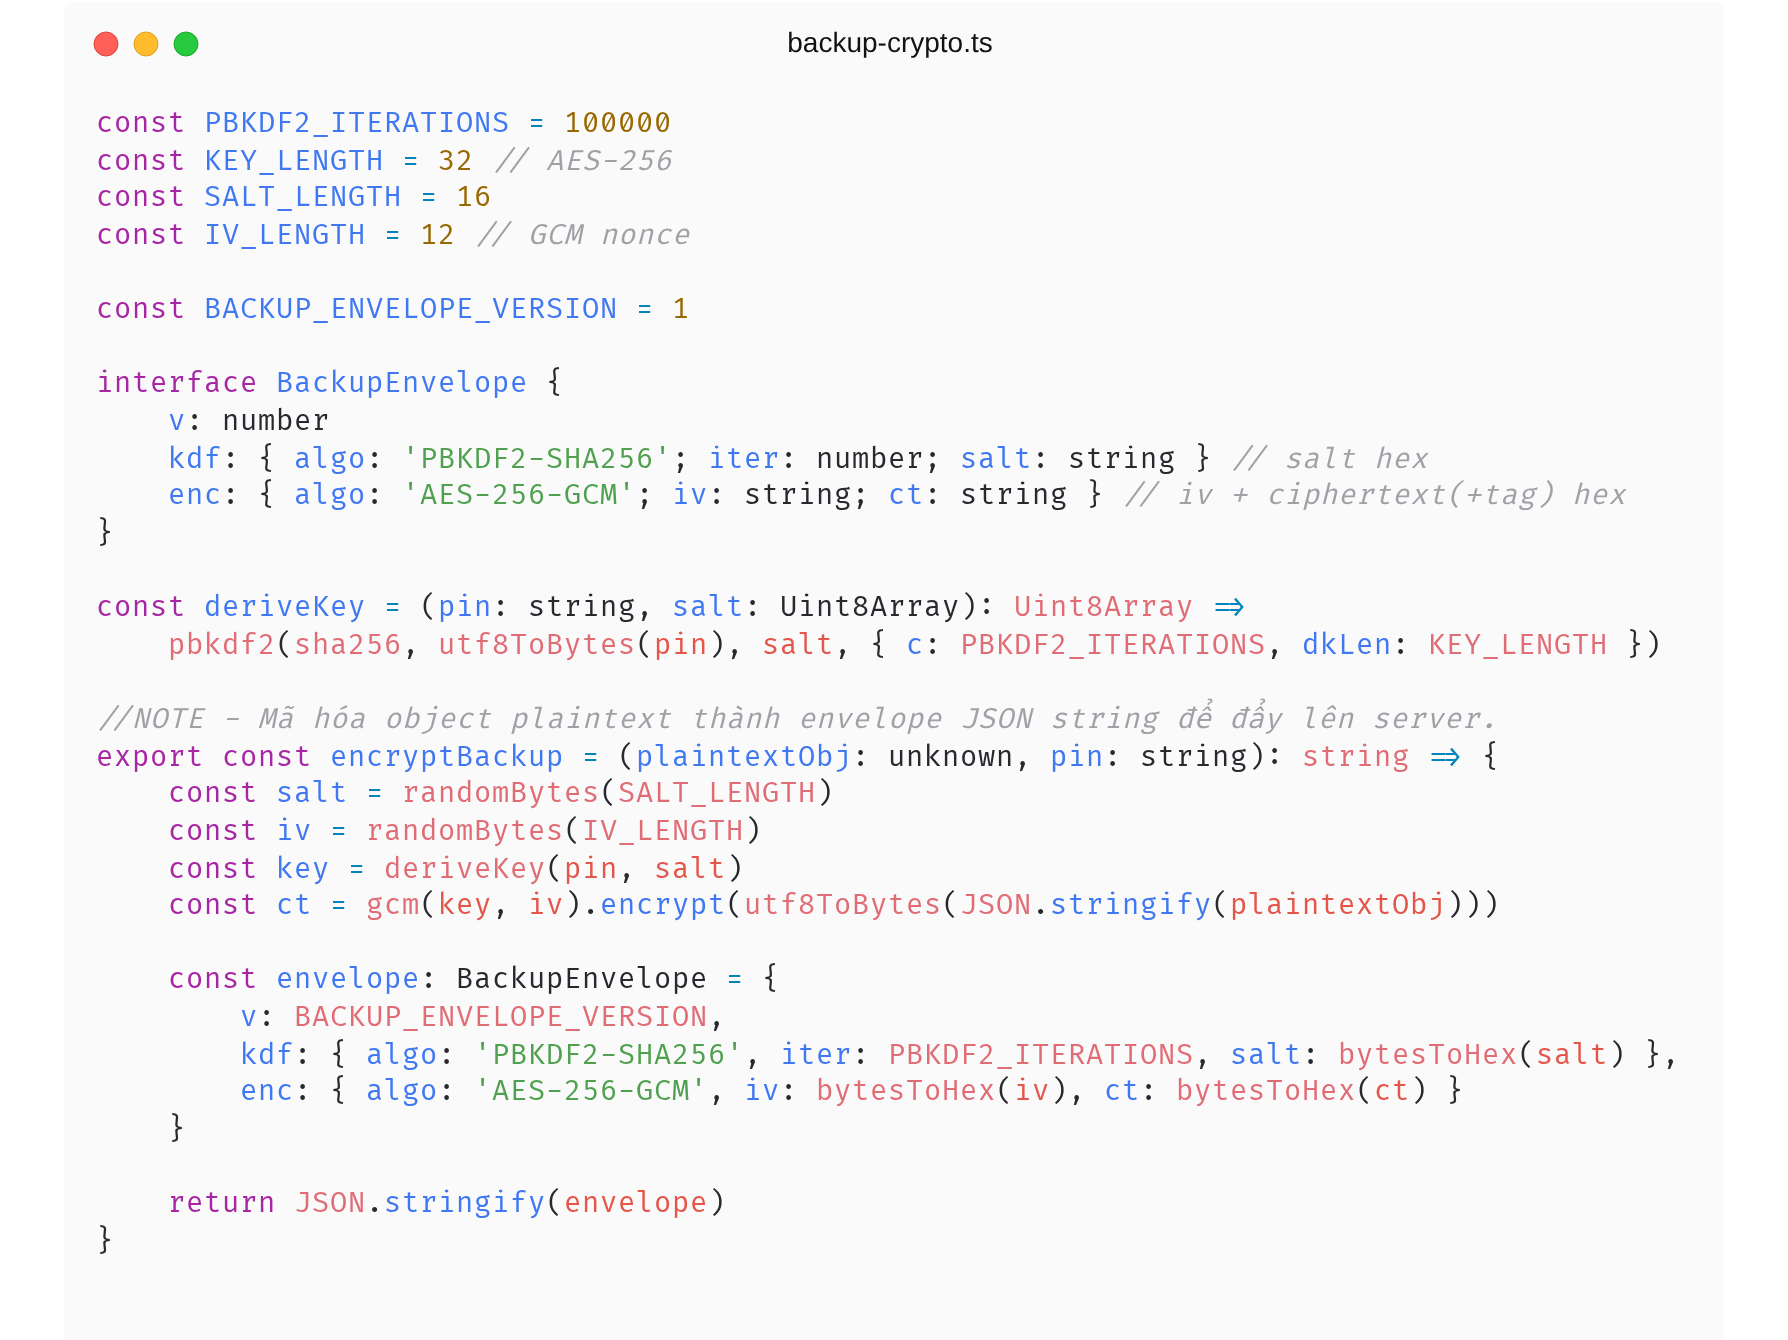
\includegraphics[width=\textwidth, keepaspectratio]{Figures/code/backup-derive-key.png}
    \caption{Hàm dẫn xuất khóa từ mã PIN bằng PBKDF2-SHA256 và mã hóa gói sao lưu bằng AES-256-GCM phía máy khách}
    \label{fig:backup-derive-key}
\end{figure}

\subsubsection{Lớp mã hóa dữ liệu khi lưu trữ (\textit{at-rest encryption}) phía máy chủ}

Khi nhận được gói envelope, Identity Service áp dụng thêm \textbf{một lớp mã hóa thứ hai} trước khi ghi xuống MongoDB nhằm bảo vệ dữ liệu khi lưu trữ. Lớp này dẫn xuất khóa bằng \pkg{argon2id} từ một bí mật phía máy chủ \pkg{BACKUP\_SECRET} kết hợp một salt ngẫu nhiên theo từng bản ghi, rồi mã hóa bằng \pkg{AES-256-GCM}. Như vậy, một bản sao lưu chịu hai lớp mã hóa độc lập: lớp ngoài chỉ giải được bằng mã PIN của cử tri, lớp trong chỉ giải được khi máy chủ nắm \pkg{BACKUP\_SECRET}. Kẻ tấn công đọc trộm cơ sở dữ liệu sẽ không thu được gì nếu thiếu cả hai bí mật này.

\subsubsection{Khôi phục và lưu ý vận hành}

Khi khôi phục, Identity Service gỡ lớp mã hóa dữ liệu khi lưu trữ và trả lại gói envelope nguyên bản do máy khách tạo; ứng dụng dẫn lại khóa từ mã PIN và giải mã. Nhờ \pkg{AES-256-GCM} là mã hóa có xác thực (\textit{authenticated encryption}), một mã PIN sai sẽ khiến bước kiểm tra thẻ xác thực thất bại ngay tại máy khách và ứng dụng báo lỗi ``Mã PIN không đúng'' — máy chủ không tham gia và cũng không học được bất kỳ thông tin nào về mã PIN.

Về vận hành, biến môi trường \pkg{BACKUP\_SECRET} của Identity Service phải được đặt bằng một giá trị mạnh trong môi trường sản xuất; giá trị mặc định dự phòng chỉ phục vụ phát triển cục bộ. Lý tưởng nhất, bí mật này nên được quản lý bởi một kho bí mật chuyên dụng thay vì lưu trong tệp cấu hình.

\input{Chapter-3/3.15-Ket-luan-chuong}

\newpage

\phantomsection\addcontentsline{toc}{section}{\numberline {}TÀI LIỆU THAM KHẢO}
% \bibliographystyle{IEEEtran}
% \bibliography{References}
\begin{thebibliography}{00}
\bibitem{b1} abc
\bibitem{b2} xyz
\end{thebibliography}

\newpage
\section*{PHỤ LỤC}
\phantomsection\addcontentsline{toc}{section}{\numberline{} PHỤ LỤC}
\setcounter{section}{1}
\setcounter{subsection}{0}
\section*{PHỤ LỤC 1}\label{pl:dac}

\end{document}
